\documentclass[11pt]{book}
\usepackage{amsmath} %Never write a paper without using amsmath for its many new commands

\usepackage{amssymb} %Some extra symbols

\usepackage{makeidx} %If you want to generate an index automatically
%\usepackage{graphicx} %If you want to include postscript graphics
\ifx\pdftexversion\undefined
\usepackage[dvips]{graphicx}
%%%%%%%% 
%% To include .jpg and .pnm into latex
%%%%%%%%%%%%%%
\DeclareGraphicsExtensions{.jpg,.eps,.pnm}
\DeclareGraphicsRule{.jpg}{eps}{.jpg.bb}{`jpeg2ps -h #1}
\DeclareGraphicsRule{.pnm}{eps}{.pnm.bb}{`pnmtops #1}
\else
\usepackage{graphicx}
\fi
 
\usepackage{epsfig}

\usepackage{color}  %Add color capabilities to fonts,e.g. \color{blue}{text something}
\usepackage{listings} % Add typeset programs (programming code) within LaTeX.

\usepackage{tabularx}
%\usepackage{ucs}
\usepackage[T1]{fontenc}
%\usepackage[utf8]{inputenc}
\usepackage{lmodern}

\usepackage{chemarr}

\usepackage{verbatim}

\usepackage[version=3]{mhchem}

%\usepackage{mystyle} %Create your own file, mystyle.sty where you put all your own \newcommand statements, for example.
%\usepackage{url}
\usepackage[hyphens]{url}
           % usage \url{URL}

\usepackage[hypertex, dvips]{hyperref}       % does not work with LaTeX2HTML
            % usage \href{URL}{text}
%\includeonly{chaptr2} %If you just want to process chaptr2.tex

\usepackage{breakurl}  % used with dvips, not with pdflatex

\usepackage[all]{hypcap}
%\graphicspath{{./images/}}

%\usepackage{lgrind}
\usepackage{framed}
%\usepackage[square]{natbib}
\usepackage[square,sort,comma,numbers]{natbib}
\usepackage{multicol}
\usepackage[style=2]{mdframed}


\begin{document}

\author{Tuan, Hoang-Throng}
\title{R statistic programming language}
\date{Jan 2009}

\frontmatter
\tableofcontents
%\include{preface}

\mainmatter
\lstset{language={R}, numbers=left, numberstyle=\tiny,
  stepnumber = 5, numbersep=5pt, keywordstyle=\color{blue}}

\def\ci{100\%\times (1-\alpha)}
\def\pr{\text{Pr}}
\def\pval{p-\text{value}}
\def\max{{\text{max}}}

\part{Statistics}

\chapter{Introduction}
\label{chap:introduction}

\section{Steps by steps to R}

\begin{enumerate}
  \item If you haven't installed R, read Sect.\ref{sec:R-install}
  
  \item Once you open R GUI: a prompt will show 
\begin{verbatim}
>
\end{verbatim}
where we can type in commands. 

NOTE: Of course, we can also run from a script file


  \item Type in the first few commands: execute a function

In R, in order to be executed, a function always needs to be written with parentheses, even if there is nothing within them
\begin{verbatim}
> ls()
\end{verbatim}

If one just types the name of a function without parentheses, R will display the content of the function.

  \item To get help (Sect.\ref{sec:getting-helps}), at any time, from the
  prompt, type
\begin{verbatim}
help.start()
\end{verbatim}
  
  \item R is a language which is both a functional language
  (Sect.\ref{sec:R-functional}) and an object-oriented language
  (Sect.\ref{sec:R-object-oriented})
  
variables, data, functions, results, etc, are stored in the active memory of the
computer in the form of {\bf objects} which have a name.
Functions  are themselves objects. We access to an object via its name. We
manipulate an object by calling operators (arithmetic, logical, comparison, ...)
and functions.


  \item Type in the first few commands: assigmnent to create a named-object
  
While R is running, variables, data, functions, results, etc, are stored in the
active memory of the computer in the form of objects which have a name.

  

R is an interpreted language, not a compiled one, meaning that all commands
typed on the key- board are directly executed without requiring to build a
complete program like in most computer languages (C, Fortran, Pascal, \ldots)

  \item 

\end{enumerate}


\section{History of R}
\label{sec:history-r}

S is a statistical programming language built to run on GCOS operating
system (target to mainframe computers
only)\footnote{\url{http://cm.bell-labs.com/cm/ms/departments/sia/S/history.html}}.
The aim of the language, ``to turn ideas into software, quickly and
faithfully'' as expressed by John Chambers (who invented S).

S is a {\it functional language}, and methods in the language are
function-based, not class-based.  There are two implementation of S:
the freeware, R, and the commercial software, S-PLUS.

R is open-source software which implements the S programming language
using C and FORTRAN, with some modification, i.e. its semantics are
derived from Scheme programming language. Scheme is a multi-paradigm
programming language derived from LISP. 

\begin{mdframed}

NOTE: Here is the list of different programming paradigms:

\begin{itemize}
\item dataflow (e.g. spreadsheets like Excel) 
\item visual programming language (e.g. Simulink)
\item functional programming language (e.g. Perl)
\item procedural programming language (e.g. Pascal, C)
\item object-oriented (OO) \~{} parallel computing (e.g. C++, Fortran 2003,
  Java, C\#)
\item constraint programming (e.g. Prolog)
\item declarative programming (e.g. HTML)
\end{itemize}
\end{mdframed}

\textcolor{blue}{So, the R language is a two-paradigm programming
  language}.
Beside as a functional language (Sect.\ref{sec:R-functional}), R now supports
class-based method (Object-Oriented) - Sect.\ref{sec:R-object-oriented}.

Current R is compatible with version 4 of S, S4, which provides
advance OO features since classes of S4 differ markedly from S3
classes. Version 4 has been developed since 1998 (add formal
class-method model, connections, large objects), 1999 (interfaces to
Java, Corba).


Wiki: ``{\it Up to this date, much of the statistical computing was done by
directly calling FORTRAN subroutines; however, S was designed to offer
an alternate and more interactive approach}''


\textcolor{blue}{One of the most important things in R to remember is
that every thing is an object, even for functions and expressions (a
value, a variable, a vector or matrix, a dataset)}.
An object is determined by 2 criteria:

\begin{itemize}
\item MODE\label{mode}:
  {\it logical, complex, factor, numeric, character, list,
    raw, any},
  and {\it function}. The MODE of an object is automatically
  determined by the types of things stored in it.

\item CLASS\label{class}: [vector] matrix, array, data.frame, and hundreds of
  special classes created by specific functions. The CLASS of an
  object is set by default depending on how it was created. However,
  it can be changed explicitly, since it is a way that determines how
  functions deal with the object. Depending on the object's CLASS, the
  object will behave differently in different functions.

\end{itemize} 

A collection (database) of objects is tended to be called
{\it libraries} if the objects are mainly functions. In R, for
functions, there is no 'pass by reference' parameters, only 'pass by
value'.  'A graphics are written out and are not stored as
objects'. Thus, the only way to save a figure is to open a connection
to the device (files, printer, ...)  before do any plotting
operation. For example, save the figure to a postscript format:
\begin{lstlisting}
postscript("filename.eps")
plot(x,y) 
dev.off()
\end{lstlisting}


\subsection{functional aspect of R}
\label{sec:R-functional}


Variables, data, functions, results, etc, are stored in the active memory of the
computer in the form of {\bf objects} which have a name. A function is also an
object in R.

Executing a function needs (1) arguments; and (2) options (which are arguments
with default values), and this returns a result.
\begin{itemize}

  \item The arguments can be objects (“data”, formulae, expressions, . . . ),

An R function may require no argument: either all arguments are defined by
default (and their values can be modified with the options), or no argument has
been defined in the function.

\end{itemize}

The basic of understanding a functional languge is to know how an assignment works

\subsection{-- quotes in R: single, double quotes or backtick}


Three types of quotes are part of the syntax of R: single and double quotation
marks and the backtick (or back quote, `)

\url{https://stat.ethz.ch/R-manual/R-devel/library/base/html/Quotes.html}

\subsection{-- creating the first object using assignment in R}

As 'x' is a name, assigning a value to it can be done via different ways:
two of them have leftwards and rightwards forms.
The name x can be a name or an expression defining a part of an object to be
replaced (e.g., \verb!z[[1]]!)

\begin{verbatim}

x <- value
x <<- value

value -> x
value ->> x

x = value
\end{verbatim}

EXPLAIN:
\begin{enumerate}
  \item  The operator \verb!<-! can be used anywhere, 
  
  \item whereas the operator \verb!! is only allowed at the top level 
  (e.g., in the complete expression typed at the command prompt) or as one of the subexpressions in a braced list of expressions.
  
  \item The operators \verb!<<-! and \verb!->>! are normally only used in
  functions, and cause a search to be made through parent environments for an
  existing definition of the variable being assigned.
  
  If such a variable is found (and its binding is not locked) then its value is
  redefined, otherwise assignment takes place in the global environment.
  
  \item 
  
\end{enumerate}

\subsection{-- how to manage objects in memory}



\subsection{object-oriented aspect of R}
\label{sec:R-object-oriented}

Designers of R language try to combine aspects of {\it functional} and {\it
object-oriented} (i.e., method-centered)
approaches'\footnote{\url{http://cm.bell-labs.com/cm/ms/departments/sia/S/history.html
}}.

\begin{mdframed}

Central to any object-oriented system are the concepts of class and method. A
class defines the behaviour of objects by describing their attributes and their
relationship to other classes. The class is also used when selecting methods,
functions that behave differently depending on the class of their input. Classes
are usually organised in a hierarchy: if a method does not exist for a child,
then the parent’s method is used instead; the child inherits behaviour from the
parent.
\end{mdframed}

We will explain how to work with R for those are more familiar with standard
object oriented programming languages like Python, Java, C++, PHP, Ruby, Swift.
Object oriented programming in R can be a confusing topic. \textcolor{red}{R has
three object oriented systems (plus the base types)}, so it can be a bit
intimidating.

\begin{enumerate}
  
  \item The single system that is  not quite OO, and is called {\bf base types}
  
  \item The three OO systems are: {\bf S3 classes}, {\bf S4 classes} and {\bf R5} (or reference classes}
  
\begin{verbatim}
[[S3]], [[S4]] and [[R5]].
\end{verbatim}


  \item  Be warned though what R calls ‘class’ has little to do with the mainstream idea
of classes.

  \item  In R, there are some things called {\bf S3} and {\bf S4} classes.
If you works with OO-languages like Java, Python, you are probably better off
not thinking of S3 and S4 ‘classes’ as classes like you know them. S3 and S4 are
really just a way to implement ploymorphism for static functions.
\end{enumerate}


Methods are invoked on an object using S-style notation, i.e. \verb|x$plot(y)|
invokes the {\it plot} method on the object x, passing it an argument y.


\subsection{-- S3 classes}
\label{sec:S3-classes}

Remember that R also supports functional language, i.e. functions are first-class
citizen.

S3 system implements a style of OO programming called {\bf generic-function OO}.

\url{http://adv-r.had.co.nz/S3.html}
 
IMPORTANT: This is different from most programming languages, like Java, C++,
and C\#, which implement message-passing OO. With message-passing, messages
(methods) are sent to objects and the object determines which function to call. This
is typically written in the following form
\begin{verbatim}
// object 'dot' method (arguments)

// Here 'drawRect' is a method
//   'canvas' is an object
canvas.drawRect("blue")
\end{verbatim}

In R, S3 system  has no formal definition of classes. While computation is still
done via methods, choosing what method to execute is decided by the so-called
{\bf generic function}.
\textcolor{red}{Methods are defined in the same way as a normal function, but are called in a
different way}.

Example: The primary use of OO programming in R is for print, summary and plot
methods. These methods allow us to have one generic function, e.g. \verb!print()!, that
displays the object differently depending on its type: printing a linear model
is very different to printing a data frame.


\begin{verbatim}
//drawRect is a generic-function, and once it is called, 
// the exact behavior, i.e. the method to be used is decided by the 'canvas' object
drawRect(canvas, "blue")
\end{verbatim}




\subsection{-- S4 classes}
\label{sec:S4-classes}

S4 has formal class definitions, which describe the representation and
inheritance for each class, and has special helper functions for defining
generics and methods

S4 works similarly to S3, but is more formal.

S4 also has multiple dispatch, which means that generic functions can pick
methods based on the class of any number of arguments, not just one.


\subsection{-- reference classes (RC)}
\label{sec:reference-classes}

Reference classes, called RC for short, are quite different from S3 and S4. RC
implements message-passing OO, so methods belong to classes, not functions.

\section{Install R}
\label{sec:R-install}

\subsection{R language in Mac OS/X}
\label{sec:R-install-Mac}

Download: \url{http://cran.cnr.berkeley.edu}


R 3.6.0 has 
\begin{verbatim}
- R Framework 3.6.0            - R.app GUI 1.70
- Tcl/Tk 8.6.6 for X11 (optional, needed for the tcltk R package)
- Texinfo 5.2 (optional, needed to build documentation in R packages from sources)

and requires

- Mac OS X 10.11 (El Capitan) or higher


The Cocoa GUI called R.app will be installed by default in your Applications
folder,  R framework will be installed in /Library/Frameworks, Tcl/Tk and
Texinfo will be installed in /usr/local

Note: By default the installer upgrades previous El Capitan build of R if
present. If you want to keep the previous version, use pkgutil --forget
org.r-project.R.el-capitan.fw.pkg

\end{verbatim}



\subsection{Compile R from source}
\label{sec:R-compile}

IMPORTANT: Since OS X 10.11 (El Capitan) or higher,  R is compiled using
non-Apple toolkit to provide support for OpenMP and C++17 standard features.


\section{Why R is strong?}
\label{sec:why-r-strong}

R is ‘GNU S’, a freely available language and environment for statistical
computing and graphics which provides a wide variety of statistical and
graphical techniques: linear and nonlinear modelling, statistical tests, time
series analysis, classification, clustering, etc.

There are many strong points of R:
\begin{enumerate}
\item Provide a wide variety of statistical and graphical techniques.

\item Can link and call code in C/C++/Fortran. Advanced users can
  write C code to manipulate R objects directly.

\item Highly extensible throuh the use of packages. Many users submit
  their packages written for specific purposes or specific areas of
  study and these packages can be written in different languages (R,
  LaTex, Java, C (often), Fortran (often))
  \begin{itemize}
  \item An installation of R include a core set of 1476 packages.
  \item Packages classified by subject
  areas\footnote{\url{http://cran.r-project.org/web/views/index.html}}.
  \item Recent effort to develop packages in R for Bioinformatics have
  increased: {\bf Bioconductor}
  project\footnote{\url{http://en.wikipedia.org/wiki/Bioconductor}}:
  to analyse genome data, such as Affymetrix and cDNA/Oligo packages
  (to analyze microarray data), and some other packages (list the name
  here…) to analyze SAGE, sequence, SNP data. The standard library is
  {\bf BiocLite()}.
  \end{itemize}

\item Has strong OO programming capability than other statistical
  programming language.

\item Can be used as a general matrix calculation toolbox with
  comparable results to Matlab.
\end{enumerate}


\begin{figure}[htb]
    \centerline{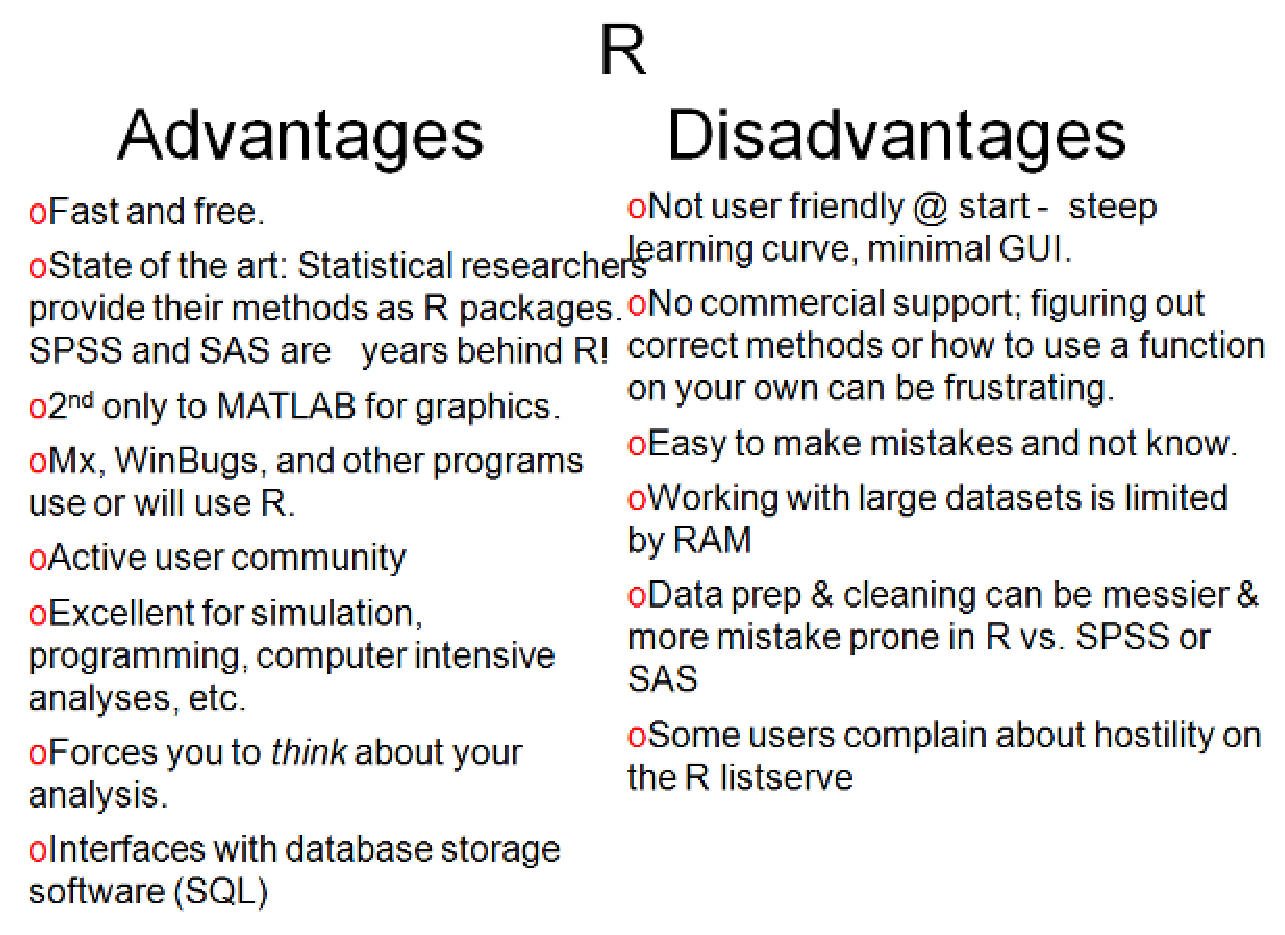
\includegraphics[height=7cm]{./images/R_strong_weak.eps}}
    \caption{Analyze R language}\label{fig:R_strong_weak}
  \end{figure}


\section{Comparison with other tools}
\label{sec:comp-with-other}


\begin{figure}[htb]
    \centerline{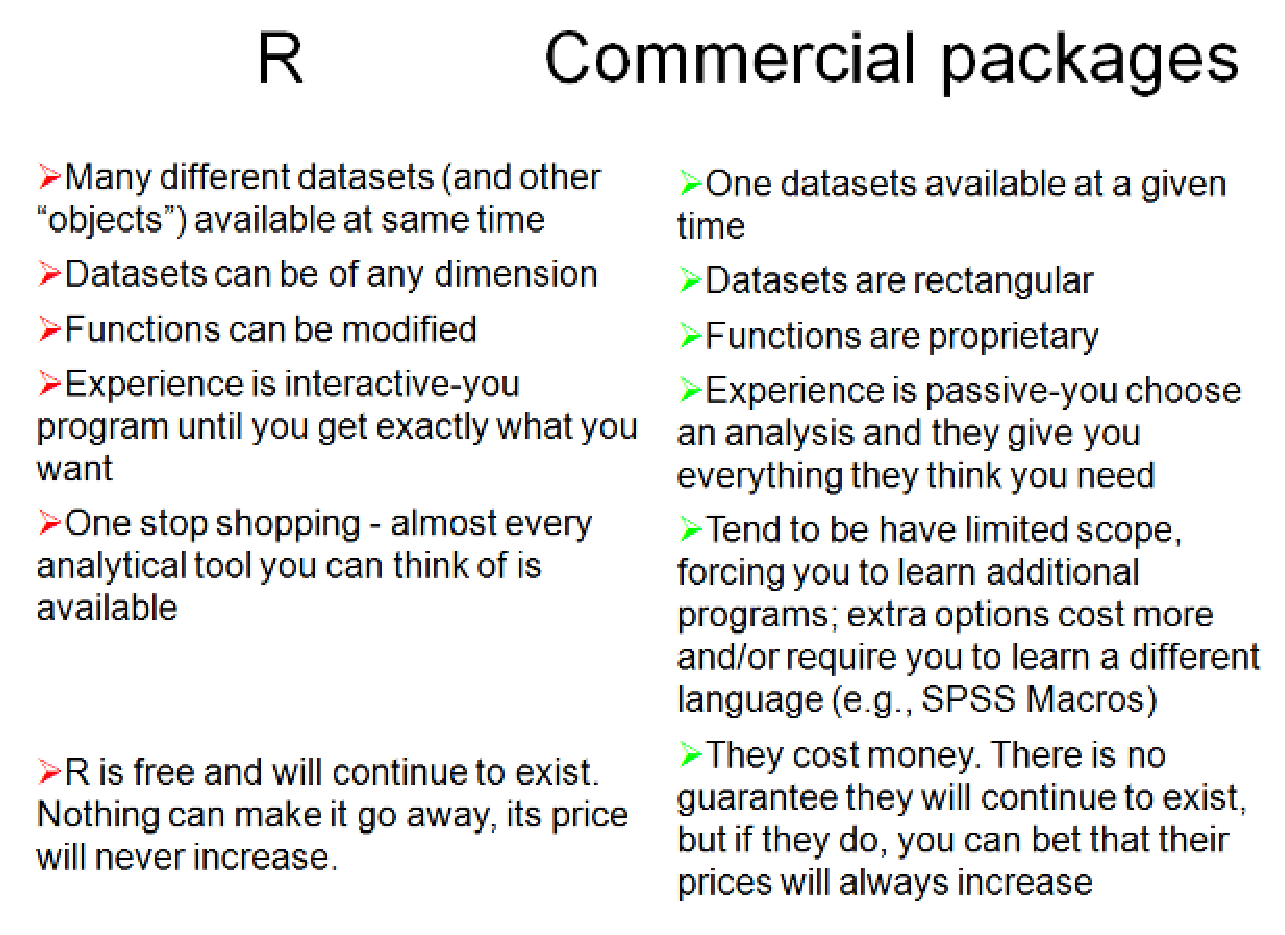
\includegraphics[height=7cm]{./images/R_others.eps}}
    \caption{Compare R language and other commercial softwares}\label{fig:R_others}
  \end{figure}


\begin{figure}[htb]
    \centerline{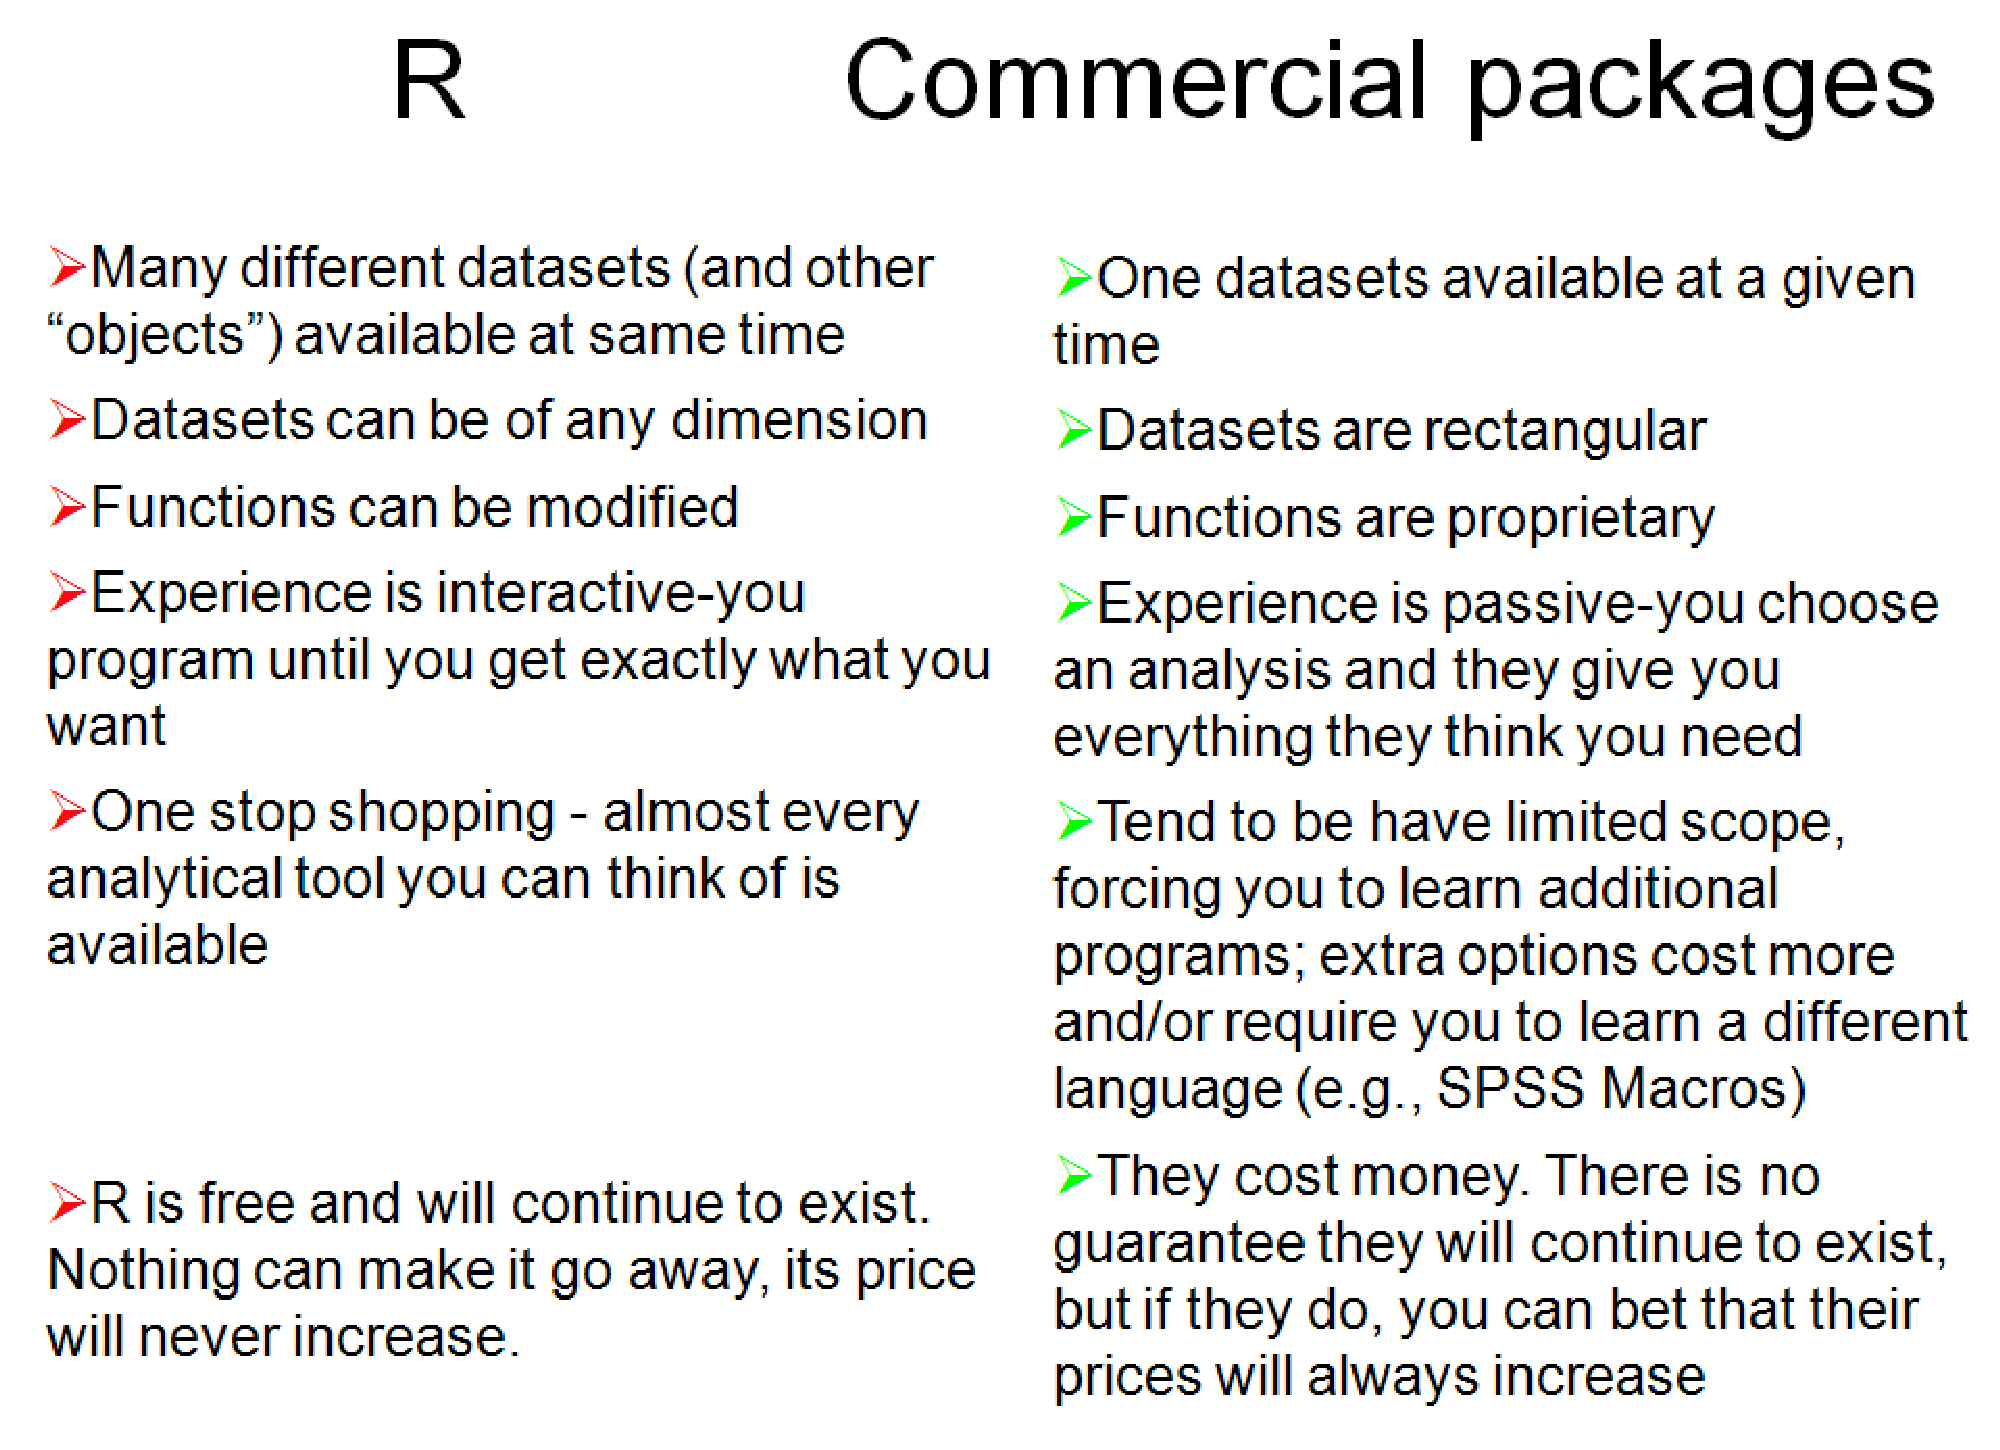
\includegraphics[height=7cm]{./images/R_SPSS_1.eps}}
    \caption{Compare R language and SAS/SPSS}\label{fig:R_SPSS_1}
\end{figure}
\begin{figure}[htb]
  \centerline{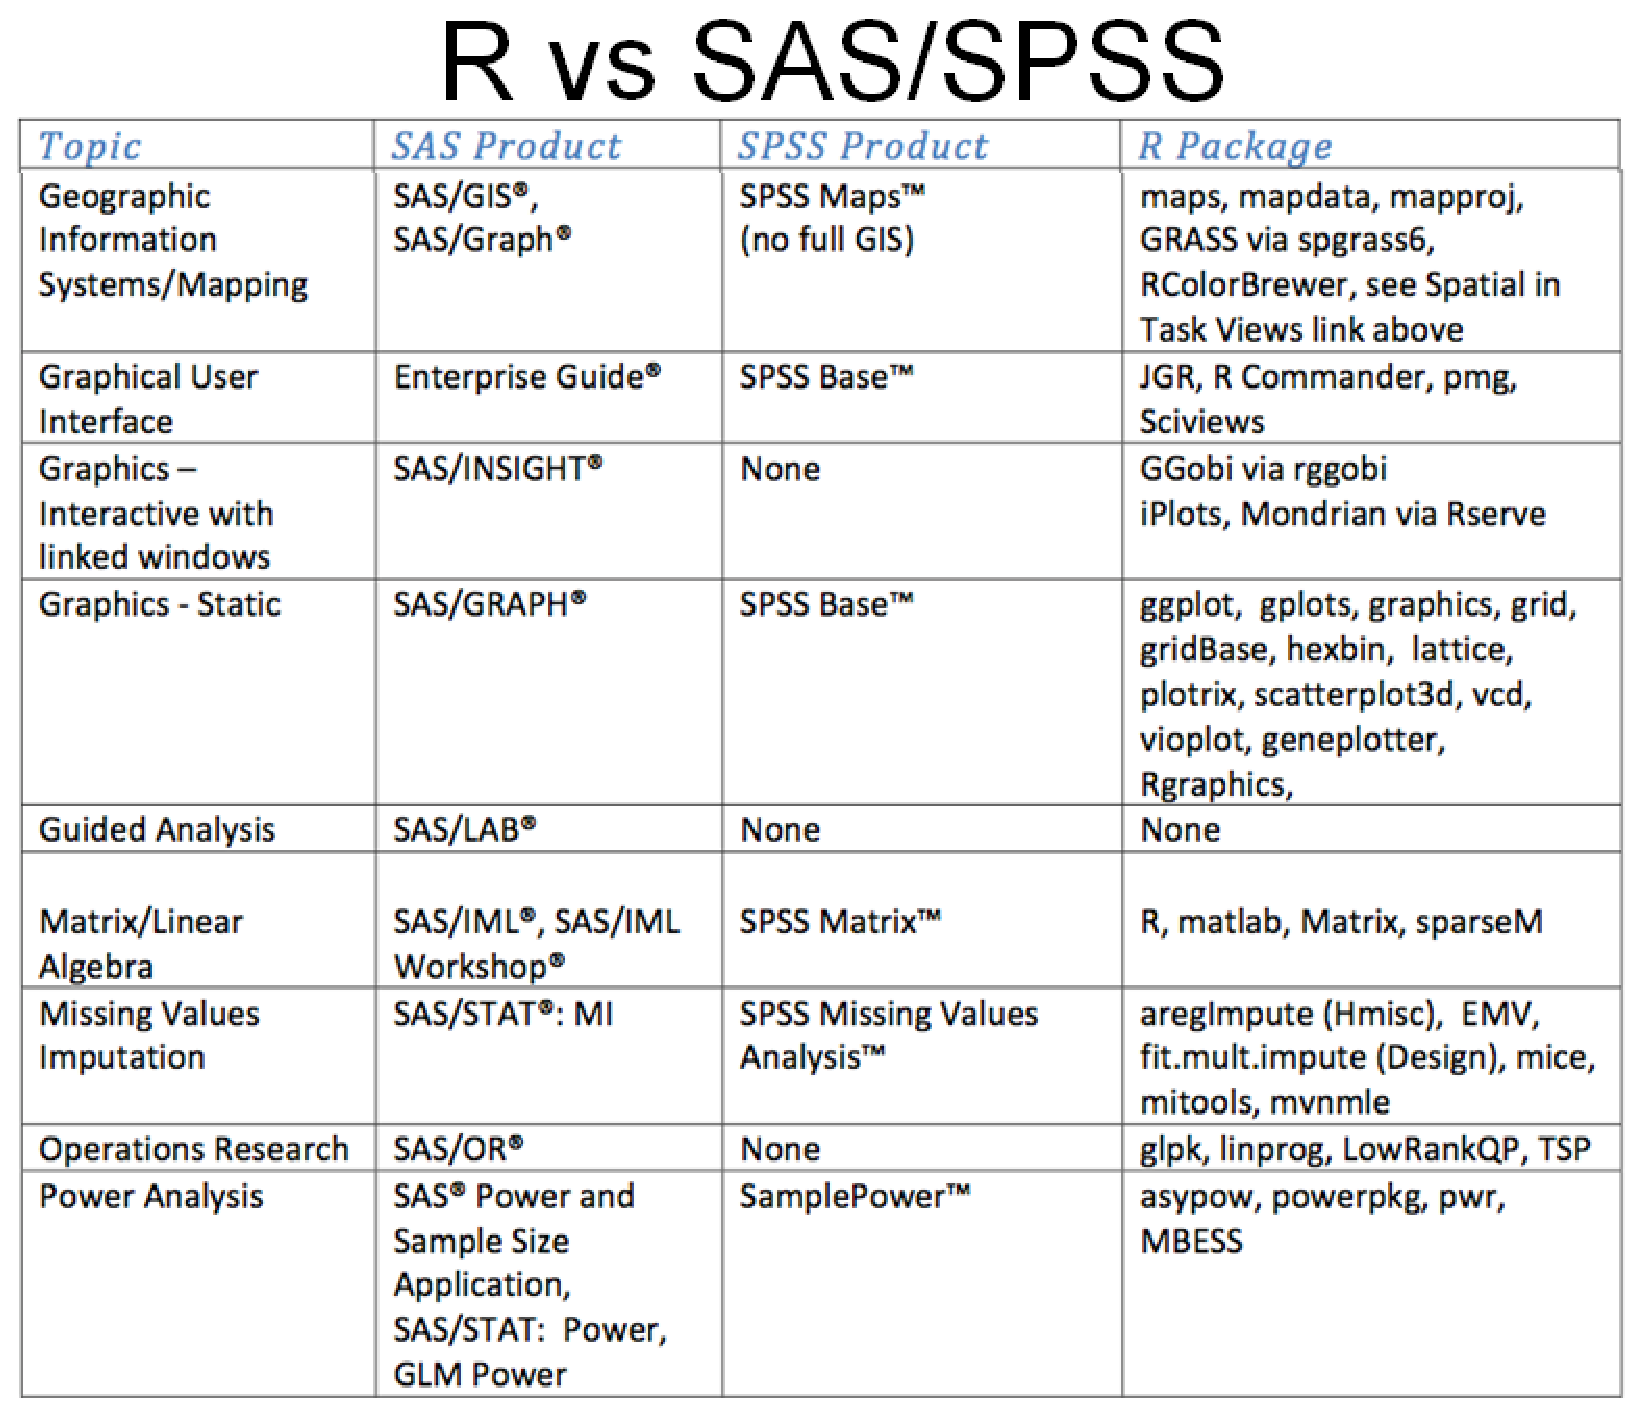
\includegraphics[height=7cm]{./images/R_SPSS_2.eps}}
  \caption{Compare R language and SAS/SPSS}\label{fig:R_SPSS_2}
\end{figure}
\begin{figure}[htb]
  \centerline{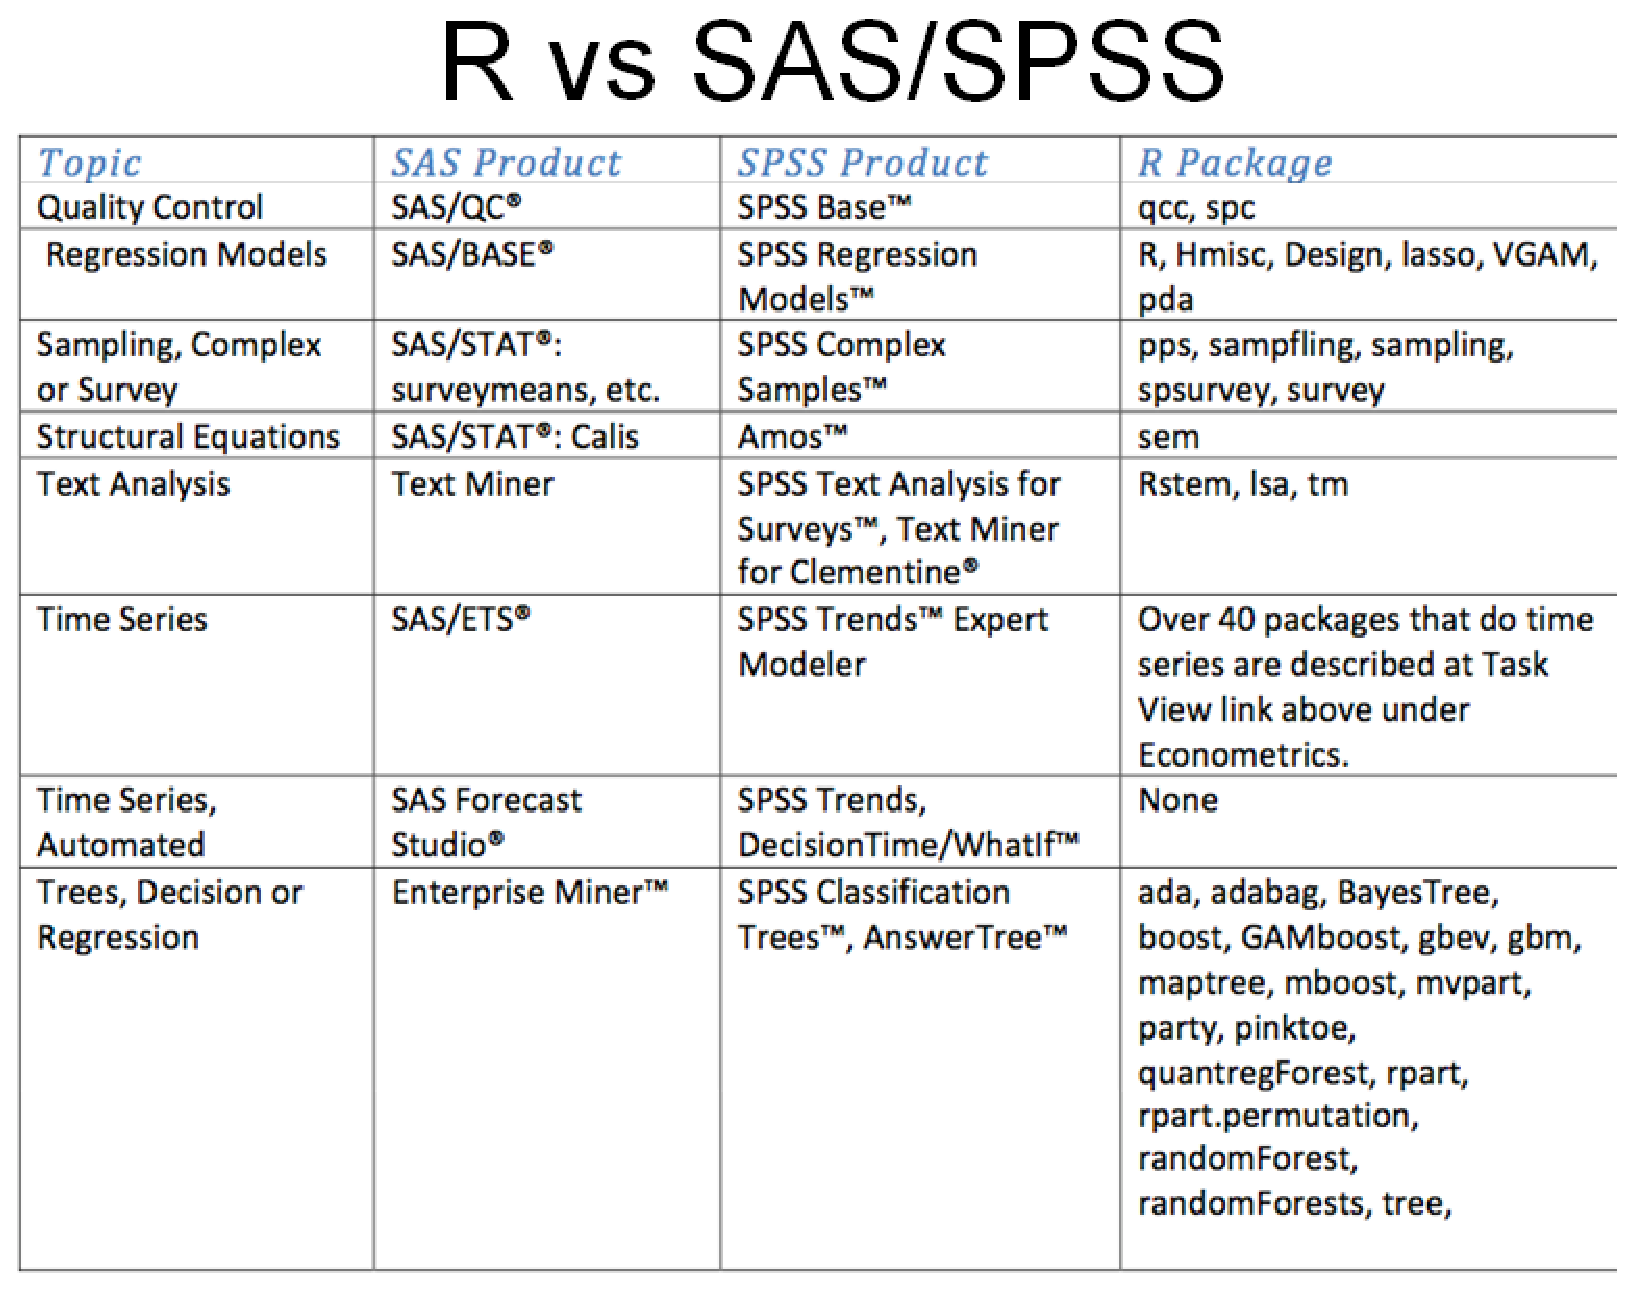
\includegraphics[height=7cm]{./images/R_SPSS_3.eps}}
  \caption{Compare R language and SAS/SPSS}\label{fig:R_SPSS_3}
\end{figure}


\section{Workspace}
\label{sec:workspace}

{\bf Namespace} is an abstract concept that hold items (variables,
objects, classes...). This is a common notion in C/C++ and some other
programming language. As a rule, names in a namespace cannot have more
than one meaning, i.e. two different items cannot have the same
name. In R, everything is put into a root namespace, called
{\bf workspace} (root working environment, global environment).

When you open R interpreter, a workspace is created. Everything you
create (variables, functions…) are stored in this workspace (workspace
acts like a directory, while variables, functions act like files). 
The namespaces of lower levels are {\it lexical environments} (scope), e.g. every
call to a function create a new evaluation frame with a lexical (local)
environment, or context created internally in the {\it call
  stack}. When a function has finished evaluating, its context is
removed from the call stack.

Here are some commands to deal with things in a workspace:
\begin{itemize}
\item To get the list of names (e.g. objects, user-defined
  functions) currently defined in this workspace, use {\bf ls()}
  or {\bf objects()} command.  
\begin{lstlisting}
>>  ls ()
>>  objects()
\end{lstlisting}

\item To remove a name from the workspace, use {\bf rm()} or {\bf
    remove()} command
\begin{lstlisting}
 >> rm (name1 [,name2]) # where name(s) can be any
         # defined objects or user-defined functions
\end{lstlisting}

\item To remove objects whose names are given in a list, you can pass
  the list to the parameter {\it list} or the {bf rm()} command,
  e.g. remove all objects or user-defined functions from the workspace

\begin{lstlisting}
        # be careful : all lower cases
>> rm (list = ls()) 
\end{lstlisting}

\item The current workspace can be saved for later use. Before you
  exit the R interpreter, you use the menu bar (File\verb|->|save workspace),
  or from the command line:
\begin{lstlisting}
>> save(name1 [, name2], file="Filename.Rdata")  # save some names only
>> save.image()           # save the whole workspace to 
      # the default file ".Rdata" in the current working directory
>> save.image(file="Filename.Rdata")
\end{lstlisting}
  where {\it name} can be any object names or user-defined
  functions

\item To save, load, or display the command line history 
\begin{lstlisting}
>> savehistory() # save to default ".Rhistory" file
>  savehistory(file="MyData.Rhistory") 
>  loadhistory(file="MyData.Rhistory") 
>  history()      # display last 25 commands
>  history(max.show=Inf) # display all commands
\end{lstlisting}

\end{itemize}

Access to the call stack is provided through a family of functions
which have names that start with 'sys.'. They are listed briefly
below.

\begin{verbatim}
sys.call
   Get the call for the specified context. 
sys.frame
   Get the evaluation frame for the specified context. 
sys.nframe
   Get the environment frame for all active contexts. 
sys.function
   Get the function being invoked in the specified context. 
sys.parent
   Get the parent of the current function invocation. 
sys.calls
   Get the calls for all the active contexts. 
sys.frames
   Get the evaluation frames for all the active contexts. 
sys.parents
   Get the numeric labels for all active contexts. 
sys.on.exit
   Set a function to be executed when the 
   specified context is exited.   
sys.status
   Calls sys.frames, sys.parents and sys.calls. 
parent.frame
   Get the evaluation frame for the specified parent context.
\end{verbatim}

\section{Getting Helps}
\label{sec:getting-helps}

Why we need help? 

\begin{itemize}
\item To have a brief view of R, we can use
\begin{lstlisting}
>> help.start()
\end{lstlisting}
  launch a web browser which shows 2 important sections:
  {\it An introduction to R} (lots of examples, tips, \& explanation),
  {\it Packages} (which has the {\bf Base} package that contains
  everything for a novice, {\bf stat} package for statistical
  functions and {\bf graphics} packages for common graphical
  visualization routines)

\item We know that functions are organized into packages. To see all
  installed packages. NOTE: not all of them are loaded in the session
\begin{lstlisting}
>>library()	
\end{lstlisting}

\item In order to use functions provided by a package, you need to
  load that package, use either {\bf library()} or {\bf require()}
  commands
\begin{lstlisting}
>> library(libName1 [,libName2])
>> require(libName)   # designed to used inside function calls
\end{lstlisting}
  with {\it libName} is the name any of the packages listed when you call
  {\bf library()}.

\item To see which packages have been loaded, you can use
  {\bf search()} command
\begin{lstlisting}
>> search()   
[1] ".GlobalEnv"    "...:stats" "...:graphics" 
[4] "...:grDevices" "...:utils" "...:datasets" 
[7] "...:methods"   "Autoloads" "package:base"     
 # to fit the page margin: "package" 
 # has been replaced by ...
\end{lstlisting}
  Each one with an indexed value.  

\item List all functions within a loaded package
\begin{lstlisting}
>> ls(pos=idx) 
\end{lstlisting}
  where {\it idx} is the index of the package found in the
  {\bf search()} command, the first index (idx=1) is always the
  {\bf .GlobalEnv}.

\item Look for function name and its meaning
\begin{lstlisting}
>> help(func_name)
>> help.search('part_of_func_name')
>> help.search("part_of_func_name")
>> ? func_name
\end{lstlisting}

\item If you don't remember the full function or object's name, you can use the
  {\bf appropos()} or {\bf find()} command
\begin{lstlisting}
>> apropos("what", where = FALSE, 
        ignore.case = TRUE, mode = "any")  
\end{lstlisting}
  return a vector of which the elements are the names of all functions
  or objects whose partial name is matching with {\it what}. To
  restrict the search, we can explicitly tell the
  \hyperref[mode]{mode}.

\begin{lstlisting}
>> find(what, mode = "any", numeric = FALSE, 
             simple.words = TRUE)
\end{lstlisting}
return a vector of which the elements are the names of all packages
matching with {\it what}. By default, {\it what} must be a complete
word in the package name; otherwise, we use {\it simple.words=FALSE}.

\item To pause/interrupt the execution, normally inside a function, so
  that user can inspect the values of objects, use the {\bf browser()}
  command
\begin{lstlisting}
>> browser()
\end{lstlisting}
Then, to continue the execution, just press {\bf c} and enter.
\end{itemize}

\subsection{Scopes}
\label{sec:scopes}

In any programming language, to allow different objects of the same
names, they are held in different abstract holders called
{\it namespace}. In addition, an object defined within a function
cannot be used out of it. We call this the scope of an object.  In the
code, whenever a symbolic name occurs, its value will be accessed by a
process called {\it scoping}, an internal search for the value of that
symbol.

In the body of a function, variables are either supplied through the
formal argument list, local variables (both are bound) or unbound
(=free). 
\begin{lstlisting}
a <- 1
f <- function() { a <- 2; a }
print (a) # 1, => a does not change, then a is unbound
\end{lstlisting}

Any variable appearing in the function body is first searched for in
the function's {\it evaluation environment}, then in its
{\it definition environment} (which has become the parent environment
({\bf enclosure}) of the former by the call of the function) and so on
up to the {\it global environment} (=root of the workspace), then
along the search path of environments until the {\it base
  package}.

(In R everything lives in (possibly nested) environments, which are a
nesting of frames (=set of local variables created in a
function). search() shows the search path.) Bound variables are
already found on the lowest level; supplied arguments are practically
treated as local. Unbound variables are not found on the lowest
level. The mentioned nesting of the evaluation environment in the
definition environment makes R's scoping lexical: The value of an
unbound variable is essentially determined by the bindings that were
in effect at the time of the creation of the function. In contrast,
with static scoping as in S, it is determined on the global
environment level. (Dynamic scoping lets it be determined by the most
recent (in time) definition, jumping up the call stack


\subsection{Generic}
\label{sec:generic}

Multiline (multi-line) statement in R is very special. You don't have
to use any special symbol to denote a multiline statement, e.g. in
2Matlab you have to specify ... at the end of the line. R statistic
automatically detect the multiline statement. However, make sure that
the operator in an expression should be on the preceding line.

Example:
\begin{lstlisting}
  4 + 4 + 
     1
\end{lstlisting}
is 9, but
\begin{lstlisting}
  4 + 4 
    + 1
\end{lstlisting}
is 8.


\subsection{Control statements}
\label{sec:control-statements}

Here, we discuss control statements:

\subsubsection{Grouped expressions}
\label{sec:grouped-expressions}

\verb!{expression_1; expression_2; …}!  
\begin{itemize}
\item return the last expression evaluated
\item similar to compound statements in C
\end{itemize}

\subsubsection{Conditions}
\label{sec:conditions}

\verb!if (…) else {…}!
\begin{verbatim}
if (expression_1) expr_2 else expr_3
\end{verbatim}
expression\_1 should return a logical value, operator \verb!||! and
\&\& may be used

\subsubsection{Test}
\label{sec:test}


\begin{lstlisting}
ifelse(test, do_yes, do_no)
\end{lstlisting}
which call \verb|do_yes| if test is TRUE, and call \verb|do_no|
otherwise.

\subsubsection{Finite loops}
\label{sec:finite-loops}

{\bf for} loops: 
\begin{verbatim}
for (name in expr_1) expr_2
\end{verbatim}

\begin{itemize}
\item name is the loop variable
\item expr\_1 is often a sequence, created by using seq() function or
  using start:end structure
\end{itemize}

\subsubsection{Infinite loops}
\label{sec:infinite-loops}


{\bf repeat} loops: 
\begin{verbatim}
repeat expr
\end{verbatim}

\begin{itemize}
\item continually evaluate expr
\item loop must be terminated using break;
\end{itemize}

{\bf while} loops:
\begin{verbatim}

while (expr_1) expr_2
\end{verbatim}

\begin{itemize}
\item while expr\_1 is FALSE, evaluate expr\_2
\item to manipulate the loop, the break; and next; statement can be
  used
\end{itemize}

\subsubsection{Next, break}
\label{sec:next-break}

 {\it next, break} statements

\begin{lstlisting}
muy = 120
sigma = 24

n = 100
x = matrix(0, nrow = n, ncol = n)
for (i in 1:n) {
  set.seed(i)
  x[i,] = rnorm(100, mean = muy, sd = sigma)
}
\end{lstlisting}

\subsection{Functions}
\label{sec:functions}

\subsection{Packages}
\label{sec:packages}

Each package may come with a set of examples (demos), we can run the
these example, to demonstrate for the usage of a particular function,
using example() function.
\begin{lstlisting}
         # get the examples on how to use a function
>> example(func_name)	
\end{lstlisting}

\section{Technical terms}
\label{sec:technical-terms}

What {\bf proportion} of men in this age group have smoked for more
than 20 years? - (i.e. what is the probability) we need to define a
r.v. X expressing the duration of smoking time for men.

What {\bf percentage} of values would fall in this range? - (i.e. what
is the probability). 


\section{Data format in R}


\subsection{data.frame}
\label{sec:data.frame-intro}


A more details of data.frame is given in Sect.\ref{sec:data.frame}.

The traditional R-based functions
\begin{verbatim}

read.table()

read.delim()

read.csv()
\end{verbatim}
import data into R as a \verb!data.frame!.


Create a data.frame
\begin{verbatim}

# create a dataframe with 4 fields
friends_data <- data.frame(name = my_friends,
         age = friend_ages,
         height = c(180, 170, 120),
         married = are_married
        )
        
        
# convert from matrix
# NOTE: t(.) can be used to transpose a matrix
class(my_data)
# --> "matrix"

my_df <- as.data.frame(my_data)
    
        
# check type
is.data.frame(friends_data)

is.data.frame(my_data)
\end{verbatim}

\subsection{-- indexing columns}


Use fieldname after \verb!$!
\begin{verbatim}
data_frame$name

# or

data_frame[, "name"]

# or a few columns using indices, or names
data_frame[, c(1, 4)]
data_frame[, c("name", "age")]


# exclude a column by using negative index

data_frame[, -1]
\end{verbatim}


\subsection{-- select rows}

Select rows in that column's data matching condition
\begin{verbatim}

# true, or false list
data_frame$age >= 27

# we can use above list of true, false to retrieve rows
data_frame[ data_frame$age >= 27, ]

data_frame[ data_frame$age >= 27, c(1, 2)]

\end{verbatim}

\subsection{-- extend/add columns}

Add a new column 
\begin{verbatim}
data_frame$new_column_name <- friends_groups
\end{verbatim}

\subsection{tibble}
\label{sec:tibble-intro}

The most modern R package \verb!readr! provides several fast functions, better
than R-based functions.
These functions import data as a \verb!tbl_df! (pronounced: tibble diff), which
is better when working with large data sets.

Tibble is a modern rethinking of R's data.frame (Sect.\ref{sec:data.frame}).

\section{R-studio (RStudio)}


\subsection{Issue after updating Java}

Issue
\begin{verbatim}
> library(rJava)
Error: package or namespace load failed for 'rJava':
 .onLoad failed in loadNamespace() for 'rJava', details:
  call: dyn.load(file, DLLpath = DLLpath, ...)
  error: unable to load shared object '/Users/kevin/Library/R/3.4/library/rJava/libs/rJava.so':
  dlopen(/Users/kevin/Library/R/3.4/library/rJava/libs/rJava.so, 6): Library not loaded: @rpath/libjvm.dylib
  Referenced from: /Users/kevin/Library/R/3.4/library/rJava/libs/rJava.so
  Reason: image not found
\end{verbatim}


\url{https://github.com/rstudio/rstudio/issues/2254}

SOLUTION: That typically needs to be run after an update of the system Java installation
\begin{verbatim}
sudo R CMD javareconf
\end{verbatim}

\subsection{Issue with memory}

\url{https://stackoverflow.com/questions/51295402/r-on-macos-error-vector-memory-exhausted-limit-reached}

\begin{verbatim}
Error: vector memory exhausted (limit reached?)
\end{verbatim}

NOTE
\begin{verbatim}
Sys.setenv('R_MAX_VSIZE'=32000000000)
\end{verbatim}
, as has been suggested on multiple StackOverflow posts, only works on the
command line, and that setting that parameter while using Rstudio does not
prevent this error:

\begin{verbatim}
• The environment variable R_MAX_VSIZE can now be used to specify 
       the maximal vector heap size. On macOS, unless specified by this 
       environment variable, the maximal vector heap size is set to the 
       maximum of 16GB and the available physical memory. This is to 
       avoid having the R process killed when macOS over-commits memory. 
       
You can set R_MAX_VSIZE to a larger value but you should do some 
experimenting to decide on a safe value for your system. Mac OS is 
quite good at using virtual memory up to a point but then gets very bad
\end{verbatim}

SOLUTION:
\begin{verbatim}
cd ~
touch .Renviron
open .Renviron

R_MAX_VSIZE=100Gb 
\end{verbatim}
This limit includes both physical and virtual memory
\subsection{O/S specific: Mac O/S, Windows, Linux}


\begin{verbatim}
> .Platform
$OS.type
[1] "unix"

$file.sep
[1] "/"

$dynlib.ext
[1] ".so"

$GUI
[1] "RStudio"

$endian
[1] "little"

$pkgType
[1] "mac.binary.el-capitan"

$path.sep
[1] ":"

$r_arch
[1] ""

\end{verbatim}

Example:
\begin{verbatim}
if(.Platform$OS.type == "windows") withAutoprint({
memory.size()
memory.size(TRUE)
memory.limit()
})
\end{verbatim}

\subsection{Options}
\label{sec:options}

There are various global options that you can adjust to fit your
needs. Use {\bf options()} command with no arguments to display the
list of available options. 

\subsection{-- set maximum memory for alloc() }

\begin{verbatim}
# call this before loading any packages

options(java.parameters = "-Xmx4024m")
\end{verbatim}


\subsection{pass data by reference?}

\url{https://stackoverflow.com/questions/2603184/can-you-pass-by-reference-in-r}



\section{R notebook}


To use a package
\begin{verbatim}
```{r}

# install a package
install.packages("tibble")


# use it
library("tibble")
```
\end{verbatim}


%%% Local Variables: 
%%% mode: latex
%%% TeX-master: "R_language"
%%% End: 

\include{Variables}
%%
%% BasicStatistic.tex
%% Login : <hoang-trong@hoang-trong-laptop>
%% Started on  Sun Jun 14 16:25:59 2009 Hoang-Trong Minh Tuan
%% $Id$
%% 
%% Copyright (C) 2009 Hoang-Trong Minh Tuan
%% This program is free software; you can redistribute it and/or modify
%% it under the terms of the GNU General Public License as published by
%% the Free Software Foundation; either version 2 of the License, or
%% (at your option) any later version.
%% 
%% This program is distributed in the hope that it will be useful,
%% but WITHOUT ANY WARRANTY; without even the implied warranty of
%% MERCHANTABILITY or FITNESS FOR A PARTICULAR PURPOSE.  See the
%% GNU General Public License for more details.
%% 
%% You should have received a copy of the GNU General Public License
%% along with this program; if not, write to the Free Software
%% Foundation, Inc., 59 Temple Place, Suite 330, Boston, MA 02111-1307 USA
%%

\chapter{Basic statistics}
\label{chap:basic-statistics}

\section{PDF (probability density function, probability distribution function)}
\label{sec:PDF}

This function provides the information about the probability (the area underling the curve, bounded by the range) 
of a random variable falling within a range (in X-axis).
So, the total area under the curve is 1.0 always. 

IMPORTANT: a probability density function can take on values greater than one, i.e. its peak can be greater than 1.

The PDF has some statistics:
\begin{enumerate}
  \item {\bf mode}: the value on X-axis at which the peaf of PDF
  
  \item {\bf mean}: just half of the two values on X-axis: mean and max values at which PDF are zeros.
  
  
  \item {\bf median}: the value on X-axis at which the underlying area on left side and right side is equal, i.e. 0.50
  
\end{enumerate}

\section{Order statistics}
\label{sec:order-statistics}


Suppose we have a sample of size $n$: $x_1,x_2,...,x_n$ from a given
distribution. Elements in this sample are sorted in increasing order to get
$x_{(1)} \le x_{(2)} \le ... \le x_{(n)}$. This sorted data is called the {\bf
order statistic} of the original sample.  The $k$-th order statistic of a sample
is equal to its $k$th-smallest value or the $k$-th element in the order
statistic. This is, along with rank statistic (Sect.\ref{sec:rank-statistics}),
the most fundamental tool in non-parametric statistics and inference.

There are some interesting properties of this order
statistics. Suppose that the original sample is obtained from the
normal distribution ($\mu,\sigma^2$), then each $x_i$ is normally distributed with
$(\mu,\sigma^2)$. However, elements in the order statistics all have
different distributions. This is due to the fact that the $i$-th element
is always not larger than the $i+1$-the element. Then, the expected
value (mean or average) of the $i$-th element must be less than or
equal that of the $(i+1)$-th element. 



\section{Quantile}
\label{sec:quantile}

The quantile concept is discussed in section
\ref{sec:sample-quant-perc}. The question is ``what is the unbiased
estimator for quantile, i.e. the $k$-th order statistic?''.

The elements in the sample are considered as empirical quantiles. To
determine the quantile corresponding to a probability level $p =
\frac{k}{q}$, the method that is largely used is to combine 2 nearest
empirical quantiles. Normally, $k$ is an integer and $q=100$. The
$k$-th q-quantile is computed as follows:
\begin{itemize}
\item $N\times \frac{k}{q}$ ($=Nk/100$) is decomposed into 2 parts:
  $j$ is the integer part, $g$ is the fractional part.
\item Type = 1:
  \begin{enumerate}
    \item If $g=0$ then the value $x_{(j)}$ is the quantile
    \item If $g>0$ then the value $x_{(j+1)}$ is the quantile
  \end{enumerate}
\item Type = 2:
  \begin{enumerate}
  \item If $g=0$, then the average of  $x_{(j)}, x_{(j+1)}$ is the
    quantile
  \item If $g>0$, then the value $x_{(j+1)}$ is the quantile
  \end{enumerate}
\item Type = 5:
  \begin{itemize}
    \item $\lambda = 1/2$ (see below)
    \item is considered the best
    \item popular among hydrologists
  \end{itemize}

\item Type = 6 
  \begin{itemize}
    \item (used by MiniTab and SPSS)  
    \item distribution-free,  but not unbiased

  \end{itemize}
\item Type = 7
  \begin{itemize}
  \item distribution-free, but not unbiased
  \end{itemize}
\item Type = 9 
  \begin{itemize}
  \item is unbiased for the normal distribution, but not for
  other distributions
  \end{itemize}
\end{itemize}



Let $\mu_{k,n}$ denote the expected value of the $k-$th order
statistic of a sample of size $n$ from a standard normal
distribution. Others name for $\mu_{k,n}$ is
{\it rankits, normal scores}, or {\it expected normal scores}. Then, a
good approximation for the rankits is
\begin{equation}
  \label{eq:13}
  \mu_{k,n} = \Phi^{-1} (\frac{k-\lambda}{n+1-2k})
\end{equation}

with $\Phi(x)=Pr(X\le x)=p$ is the normal cumulative probability, and
$\Phi^{-1}(p) = x$. In R, we use \lstinline!x = qnorm(p)!. 

The quantity $p_k = \frac{k-\lambda}{n+1-2k}$ is the intuitively
plausible and simple {\it probability level}. The most popular choice
for $\lambda$ is 0, 3/8 and 1/2. R language use 3/8 for small sample
size and 1/2 for large sample size. Then we have
\begin{equation}
  \label{eq:22}
  p_k = \frac{k}{n+1}, p_k = \frac{k-3/8}{n+1/4}, p_k = \frac{k-1/2}{n}
\end{equation}



Clearly, given a sample, the normal scores $\mu_{k,n}$ can be
computed. The {\bf normal probability plot} (rankit plot, or QQ-plot)
is the plot of the pairs $(\mu_{k,n},x_{k})$ with the normal score on
the horizontal line. If the original data comes from the normal
distribution, then the normal probability plot should be approximately
linear (slope $\sigma$ and intercept $\mu$). This is the essential
means to check an assumed normal distribution (and can be applied to
any distribution).


Now, the question is can we estimate $\sigma$ and $\mu$? These are
indeed the two parameter of the regression line. This can be done in R
as follows
\begin{lstlisting}
  ! a sample
>> x <- 5+2*rnorm(20)
  ! draw QQ-plot
>> qqnorm(x) # does a normal prob plot

>> k <- rank(x) # get ranks of x
  ! lambda = 3/8
>> q <- qnorm((k-.375)/(20+.25))

>> plot(q,x) # same as qqnorm(x)
>> lm(x ~ q) # regression coefs estimate parms
Coefficients:
         (Intercept)      q
           5.201        1.898
\end{lstlisting}
This is called {\it parametric regression on order statistic} or
parametric ROS method.


Reference: Chernoff and Lieberman for normal (1954) and generalized
(1956) probability. Hazen (1914) suggest $\lambda=1/2$. Blom (1958,
p.143) suggest $\lambda=3/8$. For plotting position in extreme-value
distribution, read Kimball (1960). For extensive set of references,
read Harter (1984), and Harter \& Wiegand (1985) for Monte-Carlo
study. Gamma distribution studied by Wilk et al. (1962). Reviews in
Barnett (1975), Lockhart and Stephens (1998)





\section{Rank statistics}
\label{sec:rank-statistics}


\section{Biased/Unbiased Estimators}
\label{sec:bias-estim}

An {\bf estimator} is a rule for calculating the estimate of a given
quantity based on observation data. If the estimate is a scalar, then
we call it {\bf point estimator}. Otherwise, we call it
{\bf interval estimator}. If the quantity to estimate is denoted as
$\theta$, then the estimator is denoted as $\hat\theta$ (add a hat to it).


So, the  estimator (i.e. the rule) for the mean of a sample is a point
estimator and the rule $\hat\theta$ is
\begin{equation}
  \label{eq:23}
  \theta = \frac{\sum x_i} {n}
\end{equation}
As we may obtain different sample, the estimate is considered as a
r.v. X, and thus the estimator is denoted as $\hat\theta(X)$, i.e. a
function of the r.v. NOTE: A function of a r.v. is a r.v. as well. 


The {\bf bias} of the estimator is defined as
\begin{equation}
  \label{eq:24}
  \text{Bias}[\hat\theta] = E[\hat\theta]-\theta = E[\hat\theta-\theta]
\end{equation}\
The mean of the sample is an unbiased estimator of the population
mean. The reason is that 
\begin{itemize}
\item if we increase the sample size, the sample
  mean will reach the population mean. 

\item if we increase the number of samples, under the law of Central
  Limit Theorem, the mean of the sample means also reach the
  population 
\end{itemize}

How about the estimator of the sample variance? 
\begin{equation}
  \label{eq:25}
  \begin{split}
    E[\frac{1}{n}(X-\mu+\mu-\bar{X})^2]=
    E[\frac{1}{n}(X-\mu)^2+\frac{1}{n}(\mu-\bar{X})^2+2\frac{1}{n}(\mu-\bar{X})(X-\mu)]
    \\
    =
    E[\frac{1}{n}(X-\mu)^2]+E[\frac{1}{n}(\mu-\bar{X})^2]+2\frac{1}{n}(\mu-\bar{X})E[(X-\mu)] 
\\
=E[\frac{1}{n}(X-\mu)^2]+\frac{1}{n}(\mu-\bar{X})^2-2\frac{1}{n}[\mu-\bar{X}]^2
\\
= E[\frac{1}{n}(X-\mu)^2] - \frac{1}{n}(\mu-\bar{X})^2 \\
= \sigma^2 - a^2 < \sigma^2
  \end{split}
\end{equation}
So, the (incorrected) sample variance is biased. So, in practice, to
make the sample variance more closed to the population variance, we
use a smaller denominator, i.e. divided by (n-1), rather than n. 

\section{Effect size}
\label{sec:effect-size}

Effect size is a simple way of quantifying the difference between two groups
that has many advantages over the use of tests of statistical significance
alone. Effect size emphasises the size of the difference rather than confounding
this with sample size


Effect size is a standard measure that can be calculated from any number of
statistical outputs. One type of effect size, the standardized mean effect,
expresses the mean difference between two groups in standard deviation units.
You'll see this reported as Cohen's d, or simply referred to as 'd.'





%%% Local Variables: 
%%% mode: latex
%%% TeX-master: "R_language"
%%% End: 

%%
%% StatisticalModel.tex
%% Login : <hoang-trong@hoang-trong-laptop>
%% Started on  Mon Jun 15 09:12:22 2009 Hoang-Trong Minh Tuan
%% $Id$
%% 
%% Copyright (C) 2009 Hoang-Trong Minh Tuan
%% This program is free software; you can redistribute it and/or modify
%% it under the terms of the GNU General Public License as published by
%% the Free Software Foundation; either version 2 of the License, or
%% (at your option) any later version.
%% 
%% This program is distributed in the hope that it will be useful,
%% but WITHOUT ANY WARRANTY; without even the implied warranty of
%% MERCHANTABILITY or FITNESS FOR A PARTICULAR PURPOSE.  See the
%% GNU General Public License for more details.
%% 
%% You should have received a copy of the GNU General Public License
%% along with this program; if not, write to the Free Software
%% Foundation, Inc., 59 Temple Place, Suite 330, Boston, MA 02111-1307 USA
%%

\chapter{Statistical models}
\label{chap:statistical-models}

A statitical model is a simplified description of data, usually
constructed from some mathematically or numerically defined
relationship.

Models are objects that imitate the properties of 'real' object, but in a
simpler and more convenient form. As the statistical model is never an exact
representation of the system, there is always a difference. The difference
between the model and 'reality' is called the {\it residuals}, and it is the key
for a deeper understanding the fitness of the model to the 'reality'.

Here are some examples of the models and the 'reality'.
\begin{itemize}
\item Architects use both paper drawing and small-scale physical
  models to imitate the properties of a building. Then, the appearance
  and other properties of the real house can be inferred from the
  model.

\item Chemists use wire-frame models of molecules (by constructing
  them or displaying them through computer graphics) to imitate the
  theoretical properties of the molecules that, in turn, can be used
  to predict the behavior of the real molecules.
\end{itemize}

A general criteria for a good model 'A good model reproduce as
{\bf accurate} as possible the relevant properties of the real object,
while being {\bf convenient} to use.' However, the collected data,
e.g. the test data in the fuel consumption example, does not cover all
the autombiles of interest; perhaps, we can use the model to mileage
of other automobiles. In other words, the goal is also to use the
model to understand or predict beyond the context of the current
data. For these reasons, useful statistical modeling cannot be
separated from questions of the design of the experiment, survey, or
other data-collection activity that produces the data.)
 
The choice of a statistical model depends on the application and on
the kinds of inference the users need to make. A general applied
criteria include simplicity; i.e. a model with fewer parameters or
explanatory variables.


\section{Creating a statistical model}
\label{sec:creat-stat-model}

Creating a statistical model is a multistage process.
\begin{enumerate}
\item Collecting data

\item Choose a candidate model (to describe some relation in the
  data) with some unknown free parameters

\item Fitting the model (usually by estimating some parameters based
  on some criteria, e.g. minimize least-quare error)

\item Summarizing the model to see what it say about the data

\item Using diagnostics (tables, verbal descriptions, and graphical
  displays) to see in what ways the model fail to fit as well as it
  should. Finally, decide whether another model should be chosen, or
  the model should be modified or it is good enough to describe the
  data.
\end{enumerate}

{\bf Example}: A formula to describe an additive model

\begin{verbatim}
        Mileage ~ Weight + Displacement
\end{verbatim}
which is interpreted as 'The Mileage consumption is modeled as Weight
plus Displacement' or the {\it response}, Mileage, can be predicted based
on the Weight of the car and the Number of miles, Displacement, the
car has been driven, as shown in Fig. \ref{fig:car_model}. These are
both linear model.

\begin{figure}[htb]
  \centerline{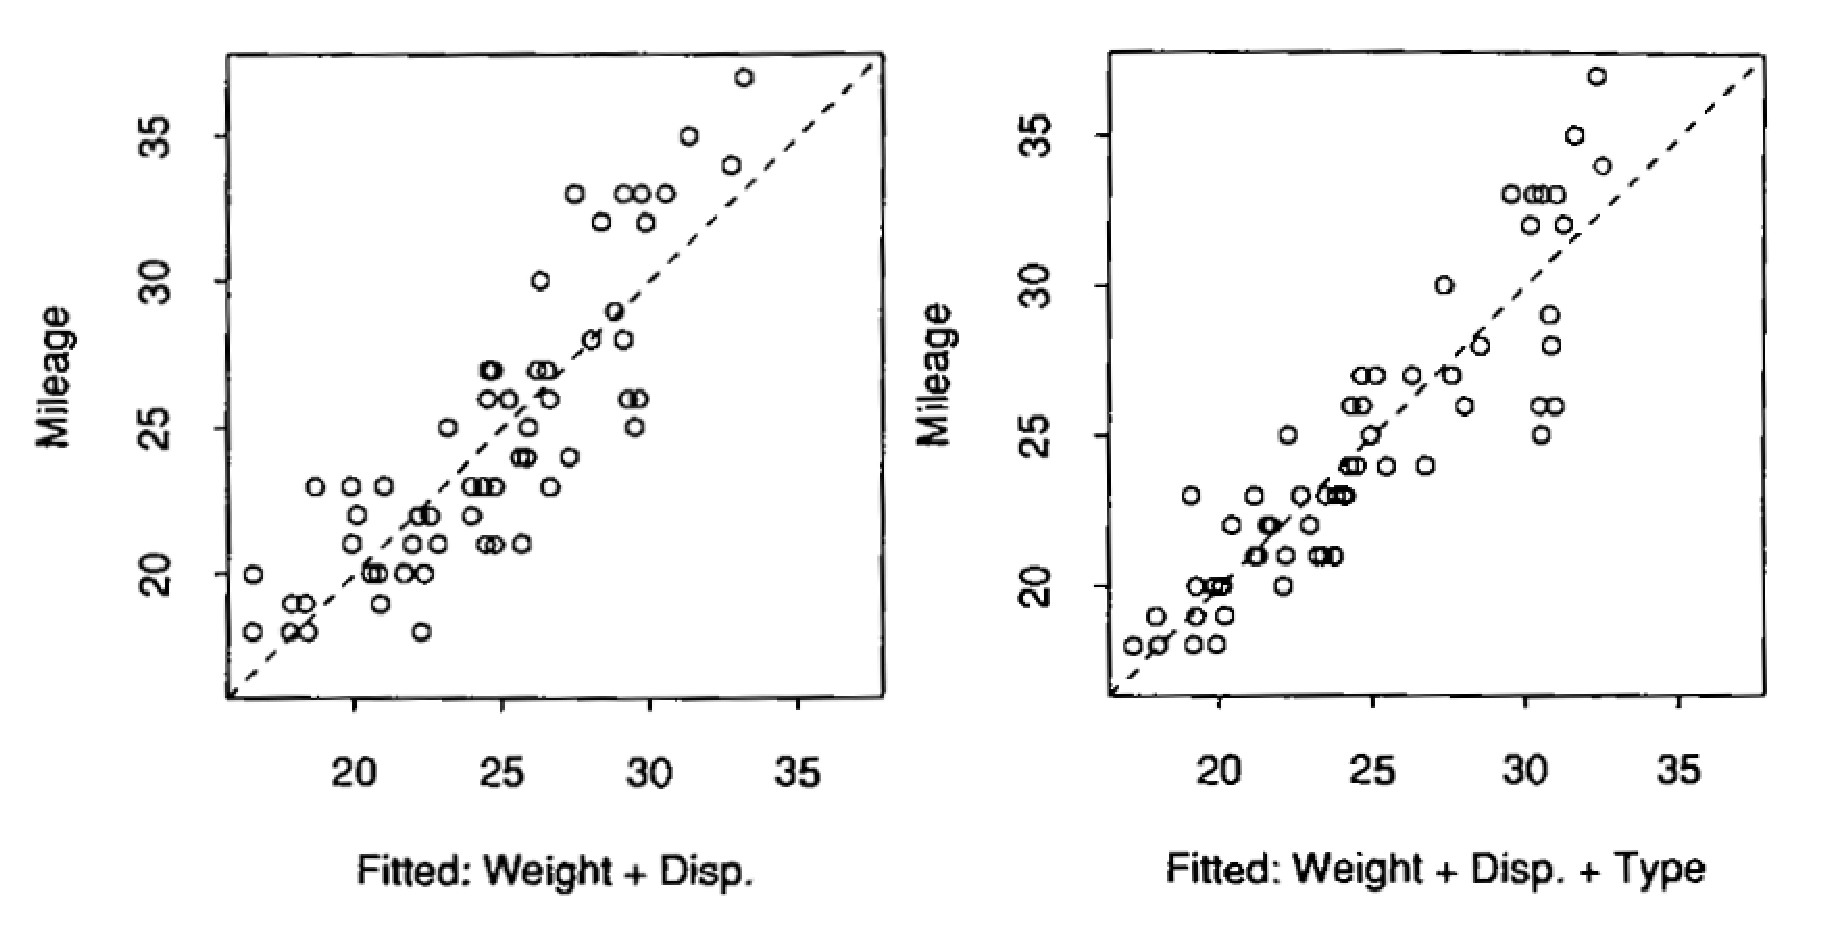
\includegraphics[height=6cm]{./images/sample_car_model.eps}}
  \caption{(a) Mileage \~ Weight + Disp; (b) Mileage \~ Weight +
    Disp + Type}\label{fig:car_model}
\end{figure}

If we plot the true value of Mileage and the values predicted by the
linear model in case (a), the model is not doing well for cars with
high mileage, i.e. they all fall above the line. However, if we add in
a coefficient for each type of car (compact, van, truck, sporty…) as
in case (b), the fit improves further. In practice, we would
continuously to study diagnostics and try alternative models, seeking
a better understanding of the underlying process.


To represent a model, R language use the concept of {\bf formula}.

\section{Error}
\label{sec:error}

Error is assumed to be normally distributed in most models

\section{A formula}
\label{sec:formula}

A statistical model tries to capture the relation, as a mathemtical function,
between the independent (explanatory) variables X1, X2, \ldots, Xn and the
response variable (dependent variable) Y: 
\begin{equation}
Y = f(X_1, X_2, \ldots, X_n)
\end{equation}
In order to produce the best models, {\bf regression analysis} is used and it
utilizes sample data (Sect.\ref{sec:regression_analysis}). 

\subsection{for a linear model}
\label{sec:linear-model}


A formula defines the structural part of a statistical model, i.e. the right
side after tilde (\textasciitilde). In order to define a formula, we need to
identify the {\bf response variable} and one or more {\bf predictor variables}.
Normally, we only have one response variable in a model, but there can be more
than one predictor.

{\bf A simple form of a formula is as follows}
\begin{verbatim}
         X ~ Y + Z
\end{verbatim}
where X is a response variable (or dependent variable); Y and Z are
two predictors (or independent variables).  This is the shorthand of
the predicting model, the '+' is not an algebraic addition, it is
being used in a special sense, to separate items in a list of terms to
be included in the model.


The form above is also similar to symbolic expression S or R. In S or
R, there is a type of object called {\bf formula} object which save
this structure. There is also a special function '\~"() that does
nothing but to save the formula as an unevaluated S expression, a
formula object.

Let's return to our basis example, the advantages of this
representation is that we don't need to specify the weighting
factors, in which the complete and correct representation should be
like this
\begin{equation}
  \label{eq:12}
  Mileage = \alpha + \beta_1 Weight + \beta_2 Disp + \varepsilon
\end{equation}
with $\varepsilon$ is the residual or the error side. There is no
information described here about how or what method should be used to
fit the model.

In R, we use the {\bf lm()} function for predicting the linear model
and the least square to compute the fitness.

\begin{lstlisting}
>> lm(Mileage ~ Weight + Fuel)
\end{lstlisting}
which is interpreted as 'Fuel is modeled as Power plus Weight' or
the response, Fuel, is represented by an additive model in two
predictors, Power and Weight.

The second point: the terms in a formula are not restricted to names
only (e.g. Weight, Fuel); they can be any S expression that, when
evaluated, can be interpreted as a variable.


{\bf Example}:If we want to model the logarithm of the Fuel, rather
than the Fuel itself
\begin{equation}
  \label{eq:17}
  \log(Fuel) \sim Power + Weight
\end{equation}

The third point: an independent variable in the formula may be a
\hyperref[sec:factor]{factor}, rather than a numeric. In the above
example, the car Type is a factor.

{\bf Example}: Consider this model where Salary and Age are numeric
vectors and Sex is a two-level factor
\begin{verbatim}
                  Salary ~ Age + Sex
\end{verbatim}
The complete representation should be as follows
\begin{equation*}
  \label{eq:18}
  Salary_i = \mu + \beta Age_i + \left\{ \begin{array}{rl}
     \alpha_M  & \text{if } Sex_i \text{ is male} \\
     \alpha_F & \text{if } Sex_i \text{ is female} \\
\end{array} \right. + \varepsilon_i
\end{equation*}
So, the two numeric values $\alpha_M, \alpha_F$ represent two levels
of Sex parameter.  This model can be represented by an equivalent one
if we create two dummy variables Xmale and Xfemale in which Xmale is
set to 1 for all male observations and 0 otherwise and Xfemale is set
to 1 for all female observations and 0 otherwise.
\begin{verbatim}
                  Salary ~ Age + Xmale + Xfemale
\end{verbatim}
Other non-numeric variables enter a model by being interpereted as
factors. Example:
\begin{itemize}
\item A logical variable is interpreted as a factor with two
  levels 'TRUE' and 'FALSE'.

\item A character variable is interpreted as a factor with levels
  equal to the set of distinct character strings

\item A category object in S or R will be treated as a factor in
  modeling software
\end{itemize}

The fourth point: a term in a formula can also refer to a
matrix. Then, each column of the matrix will appear linearly in the
model with its own coefficient. However, the entire matrix is
still interpreted as a single term.

In summary: the following S or R data types can appear in a formula
\begin{itemize}
\item a numeric vector, implying a single coefficient

\item a factor or an ordered factor, implying one coefficient for each
  level

\item a matrix, implying a coefficient for each column

\item any S expression whose evaluated results corresponding to one of
  the three types above, for example
  \begin{itemize}
  \item $(Age > 40)$
  \item cut(Age,3)
  \item poly(Age,3)
  \end{itemize}
\end{itemize}


Here are some examples of more complicated formula
\begin{itemize}
\item This is a little bit complicated formula
\begin{verbatim}
            100/Mileage ~ poly(Weight, 3) + sqrt(Power)
\end{verbatim}
  means the model needs to fit the derived variable, 100/Mileage, to a
  third-order polynomial in Weight plus the square-root of the Power
  variable.

\item A formula to fit the B-spline regression curves within two
  levels of Power obtained by cutting Power at its mid-range
\begin{verbatim}
Fuel ~ cut(Power, 2) / bs(Weight, df = 5)
\end{verbatim}

\item A nonparametric smooth curve will be used to model the
  transformed Fuel additively in Weight and Power, using 5 degrees of
  freedom for each term
\begin{verbatim}
sqrt(Fuel-min(Fuel)) ~ s(Weight, df = 5) 
                      + s(Power, df = 5)
\end{verbatim}
\end{itemize}


\subsection{for a non-linear model}
\label{sec:non-linear-model}

For nonlinear model, the formula will have to be completely explicit,
i.e. we need to specify the weighting factors. Besides, we noted that
the formula make no reference to the error $\varepsilon$ either. This
is the stochastic part of the model specification.

\section{The stochastic part of the model}
\label{sec:stoch-part-model}




%%% Local Variables: 
%%% mode: latex
%%% TeX-master: "R_language"
%%% End: 
\section{Regression analysis}
\label{sec:regression_analysis}

Regression analysis is used when the response variables and the explanatory
variables are {\it continuous}. For discrete outcome, we use {\it
classification} or {\it pattern-recognition} techniques.


The simplest and most common form is {\bf linear regression}. The goal is to
minimize loss (Sect.\ref{sec:linear_regression}) or minimize transformed loss
(Sect.\ref{sec:generalized_linear_regression}).

In the case of logistic regression (Sect.\ref{sec:logistic_regression}), it
applies to categorical (discrete) outcome by maximizing the likelihood.

An important notice is that {\bf homoscedasticity} is VERY important in the
application of regression analysis, including analysis of
variances.\footnote{\url{http://en.wikipedia.org/wiki/Heteroscedasticity}} To
test if the data is heteroscedasticity, read Chap.\ref{chap:heteroscedasticity}.

\subsection{Linear regression}
\label{sec:linear_regression}

{\bf Linear regression} is a regression analysis
(Sect.\ref{sec:regression_analysis}) technique in that the outcome (e.g.
the housing price) is a continuous-valued quantity, and is expected to be a
linear function of the input variable.

It's all about 'learning' some functional form. Suppose 
\begin{equation}
\mathbf{y} = h_\theta(\mathbf{x}) = \theta^T \mathbf{x}
\end{equation}
As a linear function, it can be represented in the matrix-vector operation.
We need to estimate the parameters (coefficients) in the transposed matrix
$\theta^T$.

\begin{mdframed}
NOTE: With $\mathbf(x) = (x_1, x_2)$, then
\begin{equation}
\mathbf{y} = h_\theta(\mathbf{x}) = \theta_0 + \theta_1 x_1 + \theta_2 x_2 = 
  \sum_{i=0}^n \theta_i x_i = \theta^T \mathbf{x}
\end{equation}
The $\theta_i$'s are the parameters
(also called weights) parameterizing the
space of linear functions.

\end{mdframed}

Example of {\bf linear regression}:
we want to predict the continuous-valued quantities (e.g., housing prices) as a
linear function of input values (e.g., the size of the house).

Here $y$ is the housing-price, and $x$ is the information about size of the
house
\begin{equation}
\begin{split}
\hat{y} &= a + b \times \mathbf{x} \\
\text{or} \\
\hat{y} &= a + b_1 \times x_1 + b_2 \times x_2 + \ldots b_n \times x_n
\end{split}
\end{equation}
with $y$ is the response variable, and $\mathbf{x}$ is the explanatory
variable which can be vectors. The two important factors: \verb!a! and \verb!b! are the
intercept and slope, respectively, in the $n$-dimensional space. The third
important factor is the correlation \verb!r!.

\begin{framed}
The validation of the linear model depends on the following assumptions of the
residual $r = (y-\hat{y})$
\begin{enumerate}
  \item Homoscedasticity (constant variance), i.e. the variance of $r$ is
  constant across the indices or the point should be evenly distributed around
  the mean. To test, we can plot $r$ vs. $y$, which if shows a dependence
  pattern then the linear model is likely INVALID. To overcome this, i.e. try to
  map to a linear model, then we can use data $\log(y)$, rather than $y$, or use
  a more complicated explanatory variables, e.g. $x_1^2$ or $x_1x_2$.
   
  \item Normality of errors, i.e. $r$ is normally distributed. Thus, RSS
  satisties $\chi^2$-distribution. The smaller RSS, the better the estimated
  model.
\end{enumerate}
\end{framed}

\subsection{-- cost function}

Now, giving the training data set
\begin{verbatim}
Living area (feet^2)   #bedrooms    Price (1000$s)
2104                   3            400
1600                   3            330
2400                   3            369
1416                   2            232
3000                   4            540
...                   ...             ...
\end{verbatim}
The question is how can we estimate the parameters $\theta$.

One reasonable method seems to be to make $h_\theta(\mathbf{x})$ close to y, we
can define the {\bf cost function} using using Least-Square Fit (i.e. minimum
square loss model)
\begin{equation}
\begin{split}
J(\theta) = \frac{1}{2} \sum_{i=1}^m \left( h_\theta(\mathbf{x}^{(i)}) -
y^{(i)}\right)^2  \\
= \sum^n_{i=1} \left( \hat{y}^{(i)} - y^{(i)}\right)^2
\end{split}
\end{equation}
%= \sum^n_{i=1} \left(y_i - \hat{y}_i \right)^2


i.e. find \verb!a! and \verb!b! to minimize the value of RSS $J(\theta)$. This
is simple Calculus I problem  with a unique minimum and unique pair (a,b) to
achieve this.
For a model with multiple input, i.e. \verb!x! is a vector like the second form
given above, this is called multiple linear regression. We still have a unique
solution, yet we now need to solve matrix algebra rather than simple algebra.

\subsection{-- R code  (R: lm function)}

\textcolor{red}{In R language}:
\begin{verbatim}
// to build the linear model
// lmFit <- lm( Y ~ X1 + ... + Xk)
// NOTE: We don't use ... but put as many Xk we want there


> lmFit <- lm( Y ~ X1 + X2 + X3 + X4)
\end{verbatim}
NOTE: We don't need to write the coefficients here. The statistics measuring the
goodness of fit and estimated coefficients of the model is given by calling
\begin{verbatim}
> summary(lmFit)

// Example output
Residuals:
Min 1Q Median 3Q Max
-1.176 -0.403 -0.106 0.524 1.154
Coefficients:
Estimate Std. Error t value Pr(>|t|)
(Intercept) 4.660 1.098 4.24 0.00082
x1 3.235 1.207 2.68 0.01792
x2 3.147 0.688 4.57 0.00043
x3 -6.486 1.881 -3.45 0.00391
x4 -1.117 0.596 -1.87 0.08223
x5 1.931 0.241 8.03 1.3e-06

Residual standard error: 0.684 on 14 degrees of freedom
Multiple R-Squared: 0.974, Adjusted R-squared: 0.965
F-statistic: 106 on 5 and 14 DF, p-value: 1.30e-10
\end{verbatim}

We can extract $\hat{y}$ vectors, i.e. of fitted values
\begin{verbatim}
> lmFit$fitted.values

> names(lmFit)   // display other names we can use
          // like fitted.values
\end{verbatim}

\subsection{-- Interview question}

In the linear regression model, the slope of the linear line is expected to be
fixed. However, in many applications, the model should be fitted by multiple
linear models, each associated with a given segment/range of data.

{\bf Interview Question}: How to modify a linear regression model to deal with
data which are linear, however the slope is time changing (for example, you can
divide the data into several segments in time, at each segment, the slope would
be found to be different), and most possibly, the slope follows a continuous
distribution, like Gaussian, for example


\subsection{Generalized Linear regression (R: glm function)}
\label{sec:generalized_linear_regression}

By transforming a variable or including interactions between the variables, we
can have more complicated linear regression models
\begin{verbatim}

log(y) ~ a + c_1 x_1 + c_2 x_1^2 + c_3 x_2 + c4 x_1 x_2
\end{verbatim}
The model is still linear as it is linear in the parameters. R language can
handle this using {\bf glm}.

\begin{framed}
For predicting a categorical outcome (such as y = true/false) it is often
advised to use a form of GLM called a {\bf logistic regression} instead of a
standard linear regression. 
\end{framed}

Example data:
\begin{verbatim}
> d <- read.table(file='http://www.win-vector.com/dfiles/glmLoss/dGLMdat.csv',
    header=T,sep=',')
> d
            x1          x2     y
1   0.09793624 -0.50020073 FALSE
2  -0.54933361  0.00834841  TRUE
3   0.18499020 -0.79325364  TRUE
4   0.58316450  2.06501637  TRUE
5   0.09607855  0.42724062  TRUE
6  -0.44772937  0.23267758 FALSE
7   1.24981165 -0.24492799  TRUE
8   0.13378532 -0.21985529  TRUE
9   0.41987141 -0.63677825 FALSE
10  1.28558918  1.37708143 FALSE
11  0.32590303  0.90813181  TRUE
12  0.01148262 -1.35426485 FALSE
13 -0.98502686  1.85317024  TRUE
14 -0.23017795 -0.06923035 FALSE
15  1.29606888 -0.80930538  TRUE
16  0.31286797  0.21319610  TRUE
17  0.03766960 -1.13314348  TRUE
18  0.03662855  0.67440240 FALSE
19  1.62032558 -0.57165979  TRUE
20 -0.63236983 -0.30736577 FALSE
\end{verbatim}

\subsection{-- Logistic regression (y=true/false)}
\label{sec:logistic_regression}

\begin{mdframed}
Example data: above \verb!y! get either true or false, which if we use a regular
linear model
\begin{verbatim}
lm(y ~ x1 + x2, data=d)
\end{verbatim}
then (behind the scences) R encodes y=true as 1 and y=false as 0 (R's default
encoded approach as an indicator). The result of fitting the model to a
categorical outcome is overly dependent on how you encoded the data as an
indicator. An example here is if the predicted value is '2', it still get the
same penalty as returning the predicted value to '0', if the true value is '1'. 
It means that the model can be penalized for being 'too right'. The solution is
to use {\bf logistic regression}, which is also a form of Generalized linear
regression (Sect.\ref{sec:generalized_linear_regression}).

\end{mdframed}

{\bf Logistic regression} is one regression analysis technique
(Sect.\ref{sec:regression_analysis}), yet it can be considered as a simple
classification problem (Sect.\ref{sec:classification}), in that we  wish to
predict a discrete variable such as predicting whether a grid of pixel
intensities represents a '0' digit or a '1' digit.

It's all about 'learning' some functional form. 
With logistic regression, i.e. two-class, we try to learn the 'sigmoid' or
logistic fuunctional form which is an S-shaped function that squash the value of
$\theta^T x	$ into the range [0,1] so that we may interpret the value of
$h_\theta(x)$ as a probability.

\begin{equation}
\begin{split}
P(y=1 | x) = h_\theta(x) = \frac{1}{1+\exp\left( -\theta^T x \right)} =
\sigma(\theta^T x) \\
P(y=0 | x) = 1 - P(y=1 | x) = 1 - h_\theta(x)
\end{split}
\end{equation}



To constrain the output always in the range [0,1], we use the sigmoid function
\begin{equation}
s(z) = \frac{1}{1+e^{-z}}
\end{equation}
The sigmoid s() has the following properties:
\begin{enumerate}
  \item s($-\infty$) = 0
  \item s($\infty$) = 1
  \item s(0) = 1/2
  \item s(-x) = 1 - s(x)
  \item x > y implies s(x) >  s(y)
  \item s'(x) = s(x)(1-s(x))
\end{enumerate}

And the new linear regression model (i.e. {\it logistic regression model}) is 
\begin{verbatim}
y = s * (a + b*x1 + c*x2) 
\end{verbatim}
Here, using the above data, the model supplies probabilities for each datum and
the 
\begin{verbatim}
m <- glm(y~x1+x2,data=d,family=binomial(link='logit'))
summary(m)
\end{verbatim}

To produce the model that is most consistent with the model, what it does is to
fit the maximum likelihood to the data, i.e. the model tends to yield  high
values on y=true samples, and otherwise. The {\bf maximum likelihood} solution
picks the coefficients $a,b,c$ to maximize
\begin{equation}
\left( \Pi_{i:y_u=\text{TRUE}} s(a+bx_{1i} + cx_{2i})\right)
\left( \Pi_{i:y_u=\text{FALSE}} s(a+bx_{1i} + cx_{2i})\right)
\end{equation}
NOTE: This is not the same as minimizing RSS in linear regression,
which is 
\begin{equation}
\sum_i \left( s \times (a+bx_{1i}+cx_{2i}) -\delta_{y=\text{TRUE}} \right)^2
\end{equation}

\url{http://www.r-bloggers.com/what-does-a-generalized-linear-model-do/}

\subsection{Lasso-based regression}
\label{sec:Lasso-regression}




\section{Fitting a linear model}
\label{sec:fitting-linear-model}


Fitting a linear model can be done easily in R statistics with {\bf
  lm(formula, data)} function (Sect.\ref{sec:linear_regression}) or {\bf
  glm(formula, data)} (Sect.\ref{sec:generalized_linear_regression}).

\begin{lstlisting}
> g = read.csv('galton-heights.csv')
 family father mother sex height nkids
1   1    78.5    67.0  M   73.2   4
2   1    78.5    67.0  F   69.0   4 
...
6   2    75.5    66.5  M   72.5   4

> lm( height ~ sex + father, data=g)
(Intercept) sexM father
34.4611 5.1760 0.4278

> lm( height ~ sex + father + mother, data=g)
(Intercept) sexM father mother
15.3448 5.2260 0.4060 0.3215
\end{lstlisting}

\begin{lstlisting}
> sum( g$height^2)
[1] 4013892> m1 = lm( height ~ sex + father, data=g)

> sum( m1$fitted^2) + sum( m1$resid^2)
[1] 4013892

> m2 = lm( height ~ sex + father + mother, data=g)

> sum( m2$fitted^2) + sum( m2$resid^2)
[1] 4013892
\end{lstlisting}

Orthogonality of fitted and residual
\begin{lstlisting}
> sum( m2$fitted * m2$resid )
[1] 4.239498e-12 -- essentially 0
\end{lstlisting}

Summary
\begin{lstlisting}
> m3 = lm( height ~ sex + father + mother + nkids, 
            data=g)
> summary(m3)
           Estimate Std. Error t value Pr(>|t|)
(Intercept) 16.18771 2.79387 5.794 9.52e-09
sexM        5.20995 0.14422 36.125 < 2e-16
father      0.39831 0.02957 13.472 < 2e-16
mother      0.32096 0.03126 10.269 < 2e-16
nkids      -0.04382 0.02718 -1.612 0.107

> anova(m3)
           Df Sum Sq Mean Sq F value Pr(>F)
(Intercept) 1 4002377 4002377 8.6392e+05 <2e-16
sex         1 5875 5875 1.2680e+03 <2e-16
father      1 1001 1001 2.1609e+02 <2e-16
mother      1 490 490 1.0581e+02 <2e-16
nkids       1 12 12 2.5992e+00 0.1073
Residuals 893 4137 5
\end{lstlisting}


\section{Bootstrap statistics}

%TODO: write bootstrap statistics


\section{Circular statistics}


\chapter{Heteroscedasticity - Homo}
\label{chap:heteroscedasticity}

Even though {\it normal distribution} is the common assumption before applying
the given test statistics, most of the methods of detecting heteroscedasticity
outlined below can be modified for use even when the data do not come from a
normal distribution. In many cases, this assumption can be relaxed, yielding a
test procedure based on the same or similar test statistics but with the
distribution under the null hypothesis evaluated by alternative routes: for
example, by using asymptotic distributions which can be obtained from asymptotic
theory, or by using resampling.

NOTE: Truely binomially distributed data is heteroscedastic. With the true mean
$p$ and variance $p(1-p)$, when we collect data and $p$ varying over the data,
then the expected observation errors is a function of the number of
observations. This causes the problem when  fitting and when attempting to
interpret coefficient significances. A first pass fix is to apply {\it
stabilizing transform}, e.g. sqrt(), arcsinh(), to make the observed variance
nearly constant over a wide range of $p$.
\footnote{\url{http://biomet.oxfordjournals.org/content/35/3-4/246.extract}}



\url{http://en.wikipedia.org/wiki/Heteroscedasticity}


\section{Park test}


\section{Glejser test}


\section{White test}


\section{Breusch-Pagan test}


\section{Goldfeld-Quandt test}

\section{Cook-Weisberg test}

\section{Harrison-McCabe test}

\section{Brown-Forsythe test}

\section{Levene test}


\section{Groups of data}

\subsection{F-test of equality of variances}

\subsection{Cochran's C test}

\subsection{Hartley's test}



\part{R language}
%%
%% Folders.tex
%% Login : <hoang-trong@hoang-trong-laptop>
%% Started on  Fri Jun 12 19:40:28 2009 Hoang-Trong Minh Tuan
%% $Id$
%% 
%% Copyright (C) 2009 Hoang-Trong Minh Tuan
%% This program is free software; you can redistribute it and/or modify
%% it under the terms of the GNU General Public License as published by
%% the Free Software Foundation; either version 2 of the License, or
%% (at your option) any later version.
%% 
%% This program is distributed in the hope that it will be useful,
%% but WITHOUT ANY WARRANTY; without even the implied warranty of
%% MERCHANTABILITY or FITNESS FOR A PARTICULAR PURPOSE.  See the
%% GNU General Public License for more details.
%% 
%% You should have received a copy of the GNU General Public License
%% along with this program; if not, write to the Free Software
%% Foundation, Inc., 59 Temple Place, Suite 330, Boston, MA 02111-1307 USA
%%

\chapter{Folders}
\label{chap:folders}


Wherever you run the R interpreter, it is the working directory of the
current workspace. Any access to any folder without the absolute path
is relatively to this folder. However, we can change it.

\textbullet Set the new working directory
\begin{lstlisting}
>> setwd(new_dir)
\end{lstlisting}

\textbullet To retrieve the full path of the working directory
\begin{lstlisting}
>> getwd()
\end{lstlisting}

{\bf Example}:
\begin{lstlisting}
setwd(paste(getwd(), "/BINF 702/Assign.02", 
           sep = ""))  # at Lab
setwd("F:/Textbooks/BINF 702/Data for BINF702")
setwd("F:\\Textbooks\\BINF 702\\Data for BINF702\\")
\end{lstlisting}

Supporting function: we need some string manipulation functions,
e.g. paste().


%%% Local Variables: 
%%% mode: latex
%%% TeX-master: "R_language"
%%% End: 

%%
%% Files.tex
%% Login : <hoang-trong@hoang-trong-laptop>
%% Started on  Fri Jun 12 19:40:46 2009 Hoang-Trong Minh Tuan
%% $Id$
%% 
%% Copyright (C) 2009 Hoang-Trong Minh Tuan
%% This program is free software; you can redistribute it and/or modify
%% it under the terms of the GNU General Public License as published by
%% the Free Software Foundation; either version 2 of the License, or
%% (at your option) any later version.
%% 
%% This program is distributed in the hope that it will be useful,
%% but WITHOUT ANY WARRANTY; without even the implied warranty of
%% MERCHANTABILITY or FITNESS FOR A PARTICULAR PURPOSE.  See the
%% GNU General Public License for more details.
%% 
%% You should have received a copy of the GNU General Public License
%% along with this program; if not, write to the Free Software
%% Foundation, Inc., 59 Temple Place, Suite 330, Boston, MA 02111-1307 USA
%%

\chapter{Files}
\label{chap:files}

Reading data into a statistical analysis system and export the result
to some other system are essential tasks.  In general, a data set is
organized in column-wise. As a matter of fact, data file should also
be organized in a format such that elements can be detected easily and
organized into columns.

If the file is a text file, each row is a record. In a single line,
there is a delimiter (tab, whitespace...)  to separate elements in a
row. Tab-separated and whitespace-separated text file is an important
part of working with R. To read/write to these text files, R provides
2 functions: {\bf read.table()} and {\bf write.table()}.

R is not really good in manipulating large-scale data. Thus, it is
recommended to use the facilities provided by other languages,
e.g. Java, Perl or Python, and then make use of the packages written
in these languages from R. Some of them includes: SJava, RSPerl,
RSPython packages from \href{http://www.omegahat.org}{OmegaHat}
project; and rJava from CRAN.

% R is not well suit for large-scale data. Thus, there are several
% packages (SJava, RSPerl, RSPython - from Omegahat project, and rJava -
% from CRAN) that allows user to integrate Python, Perl, Java... codes
% into R.

Normally, the files are {\it tab-separated} or {\it
  whitespace-separated} text files.  

\section{Excel file}

For writing to Excel file, it's best to use \verb!openxlsx! as it is not Java-depdendent.

For reading Excel file, it is best to use  \verb!readxl! package

\subsection{openxlsx}

 Through the use of 'Rcpp', read/write times are comparable to the 'xlsx' and
 'XLConnect' packages with the added benefit of removing the dependency on Java.
 
\url{https://cran.r-project.org/web/packages/openxlsx/}


\subsection{readxl package}
\label{sec:readxl-package}

Readxl and Rcpp are needed to load an .xls or .xlxs file.

\begin{verbatim}
> install.package(readxl)
# or
install.packages("tidyverse")

> library(readxl)
> readxl_example()
 [1] "clippy.xls"    "clippy.xlsx"   "datasets.xls"  "datasets.xlsx"
 [5] "deaths.xls"    "deaths.xlsx"   "geometry.xls"  "geometry.xlsx"
 [9] "type-me.xls"   "type-me.xlsx" 
\end{verbatim}


\section{Import}
\label{sec:import}

\subsection{into a vector or list}
\label{sec:into-vector-or}

You can read data from a file into a vector or a list using
{\bf scan()} command. The default is {\it whitespace-separated}
file. You can tell a different delimiter using {\it sep}
parameter. You can also skip a number of lines before starting to read
data by using {\it skip} parameter. You can also tell the maximum
number of lines of data to be read using {\it nlines} parameter.

\begin{lstlisting}
 scan(file = "", what = double(0), nmax = -1, n = -1, sep = "",
          quote = if(identical(sep, "\n")) "" else "'\"", dec = ".",
          skip = 0, nlines = 0, na.strings = "NA",
          flush = FALSE, fill = FALSE, strip.white = FALSE,
          quiet = FALSE, blank.lines.skip = TRUE, multi.line = TRUE,
          comment.char = "", allowEscapes = FALSE,
          encoding = "unknown")
\end{lstlisting}
{\it what} tells the type of data to be read (which can be either
'logical', 'integer', 'numeric', 'complex', 'character', 'raw' and
'list').

{\bf IMPORTANT}: If {\it what} is a 'list', then each line is a record
which contains length, fields and the list components which must be of
either 6 types listed.

{\it nmax} is the maximum number of values to read. By default, it
reads all. 

{\bf IMPORTANT}: If {\it what} is a 'list', then {\it nmax} tells the
number of lines (records) to read. 

\subsection{into a data.frame}
\label{sec:into-data.frame}

The data from the file is organized in table format, i.e. it can have
a header row, and row names. Thus, we have to use {\bf read.table()}
command. 

\begin{lstlisting}
read.table(file, header = FALSE, sep = "", 
           quote = "\"'", dec = ".", 
           row.names, col.names,
           as.is = !stringsAsFactors,
           na.strings = "NA", colClasses = NA, 
           nrows = -1, skip = 0, check.names = TRUE, 
           fill = !blank.lines.skip,
           strip.white = FALSE, 
           blank.lines.skip = TRUE,
           comment.char = "#",
           allowEscapes = FALSE, flush = FALSE,
           stringsAsFactors = default.stringsAsFactors(),
           encoding = "unknown")
\end{lstlisting}
By default: there is no header row (header=FALSE), the file is {\it
  whitespace-separated}. If there is a column read as character
string, we need to specify the quoting character using {\it quote}
parameter. 

As the data is in table format, it can have row names which can be
specified through a vector (using {\it row.names} assigned to a
vector), a number which tells the columns in the file that contains
row names (using {\it row.names} assigned to a column number), a
character string which is the name of a table column whose elements
are row names (using {\it row.names} assigned to a character string,
and {\it header}=TRUE). If {\it header}=TRUE, and the number of fields
in the first row is less than the number of columns in the data, then
the first column in the data is designated for row names. Otherwise,
row names are automatically numbered with 1, 2, 3.... 


\section{Export to a text file}
\label{sec:export-text-file}

The primary function is {\bf cat()}. 


\section{Export to a binary file}
\label{sec:export-binary-file}


\url{http://cran.r-project.org/doc/manuals/R-data.html}

%%% Local Variables: 
%%% mode: latex
%%% TeX-master: "R_language"
%%% End: 

%%
%% DataTypes.tex
%% Login : <hoang-trong@hoang-trong-laptop>
%% Started on  Fri Jun 12 19:41:09 2009 Hoang-Trong Minh Tuan
%% $Id$
%% 
%% Copyright (C) 2009 Hoang-Trong Minh Tuan
%% This program is free software; you can redistribute it and/or modify
%% it under the terms of the GNU General Public License as published by
%% the Free Software Foundation; either version 2 of the License, or
%% (at your option) any later version.
%% 
%% This program is distributed in the hope that it will be useful,
%% but WITHOUT ANY WARRANTY; without even the implied warranty of
%% MERCHANTABILITY or FITNESS FOR A PARTICULAR PURPOSE.  See the
%% GNU General Public License for more details.
%% 
%% You should have received a copy of the GNU General Public License
%% along with this program; if not, write to the Free Software
%% Foundation, Inc., 59 Temple Place, Suite 330, Boston, MA 02111-1307 USA
%%

\chapter{Data Types (Objects)}
\label{chap:data-types}

\section{Introduction}
\label{sec:introduction}


For permanent storage, data should be stored as files in hard
drives. However, in order to analyze data, it should be read into
memory. The methods to read data from files are discussed in another
\hyperref[chap:files]{chapter}. In this chapter, we will mainly discuss
how to manipulate the objects in different data types.
To completely define an object, it needs a type and a mode. 

\subsection{Type}
\label{sec:type}

R language provides a safe way to access data via symbolic names
called objects (or variables). Each object belongs to a specific (R
internal) {\bf type} which can be determined by using the
{\bf typeof()} command.

\begin{lstlisting}
typeof(object)
\end{lstlisting}
RETURN a character string whose content is an item in the structure
'TypeTable' in 'src/main/util.c'. 


The current possible types are: {\it logical}, {\it integer}, {\it double},
{\it complex}, {\it character}, {\it raw} and {\it list}, {\it NULL},
{\it closure} (for function), special and builtin (basic functions
and operators), {\it environment}, {\it S4} (some S4 objects) and others
that are unlikely to be seen at user level ({\it symbol, pairlist,
promise, language, char, ..., any, expression,
externalptr, bytecode} and {\it weakref}).

\begin{lstlisting}
"NULL"         NULL
"symbol"       a variable name
"pairlist"     a pairlist object (mainly internal)
"closure"      a function
"environment"  an environment
"promise"      an object used to implement lazy 
                  evaluation
"language"     an R language construct
"special"      an internal function that does not 
                  evaluate its arguments
"builtin"      an internal function that evaluates 
                  its arguments
"logical"      a vector containing logical values
"integer"      a vector containing integer values
"double"       a vector containing real values
"complex"      a vector containing complex values
"character"    a vector containing character values
"any"          a special type that matches 
                   all types: there are no 
                   objects of this type
"expression"   an expression object
"list"         a list
"externalptr"  an external pointer object
"weakref"      a weak reference object
"raw"          a vector containing bytes
"S4"           an S4 object which is not 
                   a simple object
"bytecode"     byte code (internal only) ***
"..."          the special variable length 
                   argument ***
"char"         a scalar string object 
                  (internal only) ***
\end{lstlisting}
Objects of types marked with a *** are not intended to be manipulated
by users.

\subsection{Mode}
\label{sec:mode}

Besides its {\it type}, an object also have a {\bf mode}.  Modes have
the same set of names as \hyperref[sec:type]{types}, except
\begin{itemize}
\item integer, double \verb|->| mode: numeric

\item special, builtin \verb|->| mode: function

\item symbol \verb|->| mode:name

\item language \verb|->| mode: ( or call
\end{itemize}

This is normally applied for object with data structure (e.g. vector,
array, matrix...) which is composed of fundamental constituents. We
use modes to determine such constituents: numeric, complex, logical,
character, list, function, call, expression, name, etc. A mode can be
accessed via {\bf mode()} function.

\begin{lstlisting}
mode(object)
\end{lstlisting}

You can change the mode of an object via
\begin{lstlisting}
mode(object) <- "newmode"
\end{lstlisting}
A more efficient internal version of {\it mode\verb|<-|} is storage.mode(x)\verb|<-|.
\subsection{Storage mode}
\label{sec:storage-mode}

{\bf storage.mode()} is a more efficient version of mode() command.
The mode of the returned object of a function is determined by the
{\bf storage.mode()} function. It can be: logical, integer, double,
complex, character, symbol etc

\begin{lstlisting}
storage.mode(object)
\end{lstlisting}

Here, we will discuss the most important objects, in alphabet
order. To test for the data type of an object, use {\bf class()}
function

\begin{lstlisting}
>> class(object)
\end{lstlisting}

\subsection{Attributes}
\label{sec:attributes}

Even though R language is not an object-oriented (OO) language, every
object can have one or more attributes. The concept of attributes
refers to any of its property which can be of intrinsic or
user-defined, e.g.

\begin{itemize}
\item mode: see above. an intrinsic attribute

\item length: number of (highest level) elements; an intrinsic
  attribute

\item dim: used to implement arrays, matrices, data.frames

\item names: used to label the elements of a vector (/array) or list,
  or the variables of a data frame. (For one-dimensional arrays,
  dimnames[[1]] is accessed.)

\item dimnames: list of character vectors used to label the dimensions
  of an array, matrix, or a data.frame.

\item class: vector of character strings (``class names'') used for OO
  programming, e.g.  data.frame, c('ordered', 'factor') or table

\item  tsp: used for periodic time series

\item levels: for factors; of type character

\item  contrasts: for factors

\item  row.names: to label the cases of a data frame

\item  rownames/colnames: first dimnames; = row.names/names in a data frame

\item source: the source code of user defined functions

\item comment: is handled by the function comment()

\end{itemize}

\subsection{Levels}
\label{sec:levels}

An object can have elements at different levels. For example a list
whose elements are lists.
\begin{lstlisting}
z1 = c (14,5,2)
z2 = c (1 , 3, 4)
z = c (z1,z2)
\end{lstlisting}
So, $z1,z2$ are two elements at the highest level of $z$ while
$14,5,2,1,...$ are elements at a lower level.

\subsection{Associated functions}
\label{sec:associated-functions}

There are various functions to set/get these modes/types/attributes.

\begin{itemize}
\item typeof(), mode(), storage.mode(), attributes(), attr(),
  length(), dim(), names(), dimnames(), class(), tsp(), levels(),
  contrasts(), rownames(), row.names(), colnames(), 

  mostly returning a vector (a list for attributes()); comment()

\item vector(), matrix(), array(), factor(), ordered(), list(),
  data.frame(), function(), call(),expression() (note the difference
  to as.expression()), creating the respective object

\item 
\begin{lstlisting}
is.object(), is.vector(), is.array(), is.matrix(), 
is.factor(), is.ordered(), is.list(), 
is.data.frame(), is.function(), is.language(), 
is.call(), is.expression(), 
is.symbol() (=is.name()),is.null(), is.pairlist(), 
is.environment(), is.table(), is.ts(),
is.tskernel(), is.atomic(), is.recursive(), 
is.logical(), is.integer(), is.double(), 
is.real(), is.complex(), is.character(),
is.numeric(), is.na() (vectorized), 
is.nan() (vect.), is.finite(vect.), 
is.infinite (vect.): 
\end{lstlisting}
  returning logical vectors (mostly of length 1)

\item as.vector(), as.symbol() (=as.name()), as.numeric(),
  as.integer() etc, 

  attempting a coercion of objects/modes/types etc; unlist(). E.g.:
  \lstinline!x <- 1; eval(as.symbol(``x''))!
\end{itemize}

\subsection{Indexing}
\label{sec:indexing}

Several constructs in R are complicated structures that are composed
of elements. Individual elements and subsets can be accessed through
indexing operators. Indexing can be used to set/get, add/remove one or
more elements.

R has three basic indexing operators ([], [[]], \$) with syntax
displayed by the following examples

\begin{lstlisting}

     x[i]
     x[i, j]
     x[[i]]
     x[[i, j]]
     x$a
     x$"a"
\end{lstlisting}
The form [[...]] only accept a single index (integer or character),
while [...] can accept a vector.
\begin{lstlisting}
x[[4]]

x[c(2,4,1)]
\end{lstlisting}
The form \$ is applied to recursive objects (lists, pairlists) and
allows a string literal or a symbol as an index. It means that the
index cannot be an expression. Otherwise, [[expr]] has to be used.


\textbullet A vector: use [...]

\textbullet A list: use [[...]] to return a single element, [...] to
return a list of selected elements.

\textbullet In vectors, matrices: [[...]] is slightly different from
[...], as it drops any {\it names} and {\it dinames} attributes and
partial matching is used for character indices.

\textbullet (since R 2.6.0), \$ when applied to a non-recursive object
is an error.

For more detail of indexing, read the corresponding data types.

\section{Special objects}
\label{sec:special-objects}

\subsection{NULL}
\label{sec:null}

It is  used whenever there  is a need  to indicate or specify  that an
object is absent.  It should not be confused with a  vector or list of
zero  length.  

The NULL object has no type and no modifiable properties. There is
only one NULL object in R, to which all instances refer.  To test for
NULL use {\bf is.null()} function. You cannot set attributes on NULL.


\section{Array}
\label{sec:array}

Arrays are vector plus a {\it dim} attribute (dimension vector).  
Arrays are ordered-column major order.

R language supports ragged array, or jagged array in which the valid
range of one index depends on the value of another. Simply it means
that different rows have different sizes.

To manipulate data based on array margins, R provides a very powerful
function {\bf apply()} or {\bf lapply()} or {\bf sapply()}.
\begin{lstlisting}
apply(X, margin, FUN, ...)
\end{lstlisting}
where {\it margin} can be either 1, 2, or c(1,2). X is an array.
FUN is a function which can return either
\begin{enumerate}
\item a vector of length $n$, then apply() returns an array of
  dimension dim(n, dim(X)[margin])
\item a scalar, then apply() return a vector if margin is a single
  value.

\item a scalar, then apply() returns an array of dimension
  dim(X)[margin] if margin is a vector.
\end{enumerate}



\section{Boolean}
\label{sec:boolean}

\section{characters}
\label{sec:characters}


\chapter{Array/Matrix/Table-like data}


\section{data.frame}
\label{sec:data.frame}

A {\bf data.frame} is a matrix-like object in which different columns can be of
different types/\hyperref[mode]{modes}/attributes
(Sect.\ref{sec:data.frame-intro}).


Data frame also has {\it dim} attributes of length 2 (the first value is the
number of rows, the second one is the number of columns).


A data.frame usually have a {\it name} attribute for the variables
(columns) and {\it row.names} attribute for the cases (rows). 

A column is implemented as a list.  Rows and columns can have assigned
labels which can be retrieved using {\bf dimnames()} command.
\begin{lstlisting}
dimnames(data.frame)[[1]]
dimnames(data.frame)[[2]]
\end{lstlisting}
This is similar to SAS or SPSS datasets.

This data type is of particularly helpful for storing reading from
text files since spreadsheet data (from Excel …) are mostly of this
form. Here is a spreadsheet in a form of a data.frame.
\begin{figure}[htb]
  \centerline{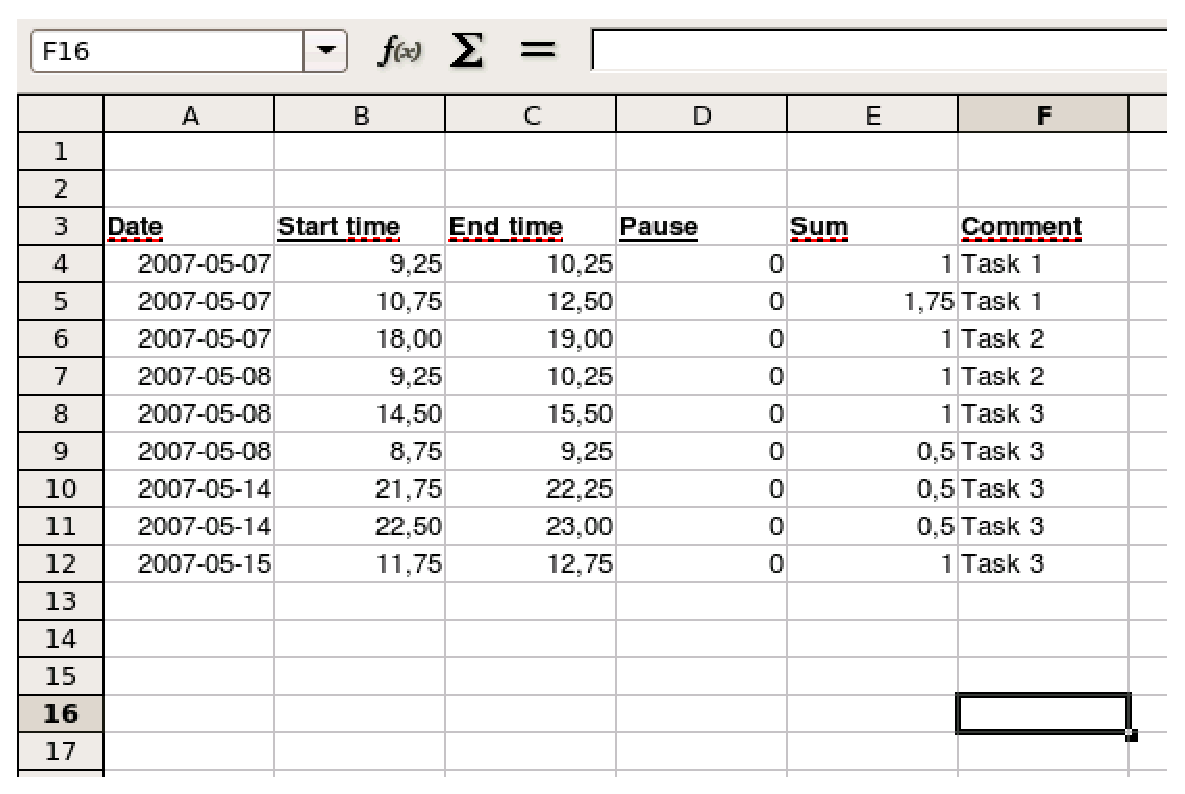
\includegraphics[height=7cm]{./images/data_frame.eps}}
  \caption{A spreadsheet}\label{fig:data_frame}
\end{figure}

Be reminding that the values of the response variable must appear on
the same column; other columns should be the value for the
corresponding independent variables. The Excel function called
{\it Pivot table} is helpful to map your data to be in the form of a
data.frame. In order for R to read the file, in Excel, you can save
the file in  'Text (Tab delimited)' format.

In fact, a data.frame is a list of variables of the same length with
unique row names. You can create a data.frame object by combining some vectors
\begin{lstlisting}
d <- c(1,2,3,4)
e <- c("red", "white", "red", NA)
f <- c(TRUE,TRUE,TRUE,FALSE)
mydata <- data.frame(d,e,f, row.names=c(4,3,'a12',5))
\end{lstlisting}

\begin{lstlisting}
data.frame(..., row.names = NULL, check.rows = FALSE,
           check.names = TRUE,
      stringsAsFactors = default.stringsAsFactors())
\end{lstlisting}
with
\begin{itemize}
\item row.names = an integer-vector giving the row names
\item check.rows = if you want each row has a unique name, set it to
  TRUE 
\item check.names = TRUE(by default), each column has a unique name.
\item stringsAsFactors = should character vectors be converted to
  Factors.  default.stringAsFactors() can be adjusted by setting
  options (stringsAsFactors = FALSE)
\end{itemize}

\subsection{Column names}
\label{sec:column-names}

Each column has its own name, to access the list of column's names you
can use {\bf names(data.frame)} or {\bf dimnames(data.frame)[[2]]}
command.

\begin{lstlisting}
>> names(mydata)
>> dimnames(mydata)[[2]]
\end{lstlisting}

The column's names can also be changed by assigning a new vector of
names to {\bf names(data.frame)}

\begin{lstlisting}
>> names(mydata) <- c("ID", "Color", "Passed")
\end{lstlisting}

\subsection{Retrieve data}
\label{sec:retrieve-data}


To access/retrieve item in an entire column, there are multiple ways
\begin{itemize}
\item use column label: \verb!data.frame$column_name!
\item use column index: \verb!data.frame[,index]!
\item use column label as column index: \verb!data.frame[column_name]!
\item exclude/remove a column by using negate value:
  \verb!data.frame[,-index]!
\end{itemize}

To access/retrieve any item (more general) from a data.frame of size
$m\times n$: since a data.frame is a column-based matrix-like data
structure, we can access

\begin{itemize}
\item the $i$-th element : \verb!data.frame[i]!

\item a range of element : \verb!data.frame[i:j]! with $0<i<j\le
  m\times n$ 

\item select all but one element $i$: \verb!data.frame[-i]!

\item slicing: including elements reside at arbitrary location
  (indicated by a vector): \verb!data.frame[c(i,j,k)]!

\item select items satisfied a logical operator:
  \verb!data.frame[data.frame > Z]! with $Z$ is any value that can be
  compared with items in the data.frame object

\item use the powerful function {\bf subset()} to select row-based
  items. RETURN: data.frame
\begin{lstlisting}
subset(x, subset, select, drop = FALSE, ...)
\end{lstlisting}
with
\begin{itemize}
\item x : either a vector, a matrix or a data.frame
\item subset : a logical expression indicating elements or rows to
    keep if the expression applied to that element (row) is TRUE
    (missing values are those that make the expression FALSE)
   
  \item select : an expression, indicating columns to select from a
    data frame or a matrix (NOT applied for vectors)
\end{itemize}
NOTE: column label can be used as variable in the expression 

\item use the {\bf with(data.frame, expr)} function: return a list of
  items in the data.frame that satisfy {\it expr}. {\it expr} is
  evaluated in a local environment constructed from data.frame
  (i.e. not in the user's workspace).
\end{itemize}

{\bf Example}:
\begin{lstlisting}
> airquality
    Ozone Solar.R Wind Temp Month Day
1      41     190  7.4   67     5   1
2      36     118  8.0   72     5   2
3      12     149 12.6   74     5   3
4      18     313 11.5   62     5   4
5      NA      NA 14.3   56     5   5
6      28      NA 14.9   66     5   6
7      23     299  8.6   65     5   7
8      19      99 13.8   59     5   8
9       8      19 20.1   61     5   9
    # select row entries from 2 columns (Ozone, Temp) 
    # with the Temp values > 80
> subset(airquality, Temp > 80, select = c(Ozone, Temp))
    # select all row entries (except entries from Temp column)
    # with Day == 1 
> subset(airquality, subset = (Day == 1), select = -Temp)
    # select all row entries (except entries from Temp column)
    # with Day > 1 and Wind < 10
> subset(airquality, subset = (Day > 1 & Wind < 10), select = -Temp)
    # select all row entries from columns 
    # starting from Ozone to Wind 
> subset(airquality, select = Ozone:Wind)
    # 
> with(airquality, subset(Ozone, Temp > 80))
\end{lstlisting}

Count the number of rows, we convert it to {\it table} data type and
use {\bf as.numeric()}
\begin{lstlisting}
X = subset(hospital,  select = c(V7,V8)) # data.frame with 2 columns

O11 = as.numeric(table(subset(X, V7 == 1 & V8 == 1)))
O12 = as.numeric(table(subset(X, V7 == 2 & V8 == 1)))
O21 = as.numeric(table(subset(X, V7 == 1 & V8 == 2)))
O22 = as.numeric(table(subset(X, V7 == 2 & V8 == 2)))

\end{lstlisting}

\section{Tibble}
\label{sec:tibble}

Tibble is a modern rethinking of R's data.frame (Sect.\ref{sec:data.frame}).


\section{factor}
\label{sec:factor}

In R, to handle nominal and ordered categorical data, a new concept
{\bf factor} is used. Example of nominal data is sex (male,
female). Example of ordered categorical data is severity of a disease
after the treatment (serious, mild, the same, better).

Each possible value of such type of data is a possible categorical
value (or level), rather than real characters or digits. Hence, a
factor in an object with a level (and optionally contrast)
attribute. Its class is {\it factor} implemented as an integer vector
with a mapped vector of names for the levels, e.g. (1,0) for (male,
female). Hence, {\it typeof(factor)} returns INTEGER,
{\it mode(factor)} returns NUMERIC.


So, the question is what it differs from category? - Factors have all
the features of categories, with some added class distinctions; in
particular, there is a distinction between factors and ordered
factors.

{\bf NOTE}: A factor with two possible values is said to be a
two-level factor.




\section{list (generic vector)}
\label{sec:list}

A list is a recursive structure, with type (Sect.\ref{sec:type}) and mode
(Sect.\ref{sec:mode}) are {\it list}. Their components can be of any type and
mode. Hence, a list is also called a {\it generic vector}.
\begin{lstlisting}
list(...)
\end{lstlisting}

Example: a list comprised of 3 vectors (Sect.\ref{sec:vector})
\begin{verbatim}
> n = c(2, 3, 5) 
> s = c("aa", "bb", "cc", "dd", "ee") 
> b = c(TRUE, FALSE, TRUE, FALSE, FALSE) 
> x = list(n, s, b, 3)   # x contains copies of n, s, b 
\end{verbatim}

A slice of a list contains one or more elements in a list.
With an index vector, we can retrieve a slice with multiple members.
\begin{verbatim}
> x[2] 
[[1]] 
[1] "aa" "bb" "cc" "dd" "ee" 

> x[c(2, 4)] 
[[1]] 
[1] "aa" "bb" "cc" "dd" "ee" 
 
[[2]] 
[1] 3 
\end{verbatim}

{\bf Direct member reference}:
Elements in a list is assessed via double bracket [[...]]] so that we can
modified it
\begin{verbatim}
> x[[2]]            # which is a vector
[1] "aa" "bb" "cc" "dd" "ee" 

> x[[2]][2]         # index the second element in the vector x[[2]]
\end{verbatim}

{\bf Named list members}: a member of a list can have a name so that it can be
referenced using name instead of the integer index.
\url{http://www.r-tutor.com/r-introduction/list/named-list-members}


\begin{lstlisting}
x[[1]] = 2
x[[2]] = c(4,2)
\end{lstlisting}


\section{matrix}
\label{sec:matrix}

A matrix is an array with {\it dim} attribute of length 2.


\textcolor{red}{Create a matrix from a vector} by casting a vector to
a matrix
\begin{lstlisting}
 matrix(data = NA, nrow = 1, ncol = 1, byrow = FALSE,
            dimnames = NULL)
\end{lstlisting}
with {\it data} is a vector. Elements in the vectors are filled in the
matrix in column-based (by default) or row-based (when byrow=TRUE).
\begin{lstlisting}
> m <- matrix(1:4, 2)
> m
          [,1] [,2]
     [1,]    1    3
     [2,]    2    4
> i <- matrix(c(1, 1, 2, 2), 2, byrow = TRUE)
> i
          [,1] [,2]
     [1,]    1    1
     [2,]    2    2
> m[i]
     [1] 1 4
\end{lstlisting}

\textcolor{red}{Create a matrix by combining old ones}: You can create
a new matrix by combining matrices/vectors in a column-wise manner or
row-wise manner using {\bf cbind(obj1, obj2...)} and {\bf rbind(obj1,
  obj2...)}, respectively. 

\begin{lstlisting}
rbind(matrix, vector1, vector2)
     # create a new matrix by adding two new vectors 
     # as two new rows

cbind(matrix, vector1, vector2)
     # create a new matrix by adding two new vectors 
     # as two new columns
\end{lstlisting}

\textcolor{red}{Transpose a matrix} use {\bf t(matrix)} function.

\textcolor{red}{Inverse matrix}: The inverse of a matrix, {\bf
  solve(matrix)} function 
\begin{lstlisting}
solve(A) ! A^{-1}
\end{lstlisting}

\textcolor{red}{Retrieve row/column size} use {\bf nrow(matrix)} and
{\bf ncol(matrix)} functions.

\textcolor{red}{Dot product} (element-by-element product) use *
\begin{lstlisting}
A * B
\end{lstlisting}

\textcolor{red}{Matrix product}, use \lstinline!%*%!
\begin{lstlisting}
C = A %*% B
\end{lstlisting}

\textcolor{red}{Cross-product} (matrix-vector product), use
\lstinline!t(A) %*% y! with $y$ is a vector,
and $A$ is a matrix. An alternative efficacy way is to use

\begin{lstlisting}
crossprod(A,y)
\end{lstlisting}

\textcolor{red}{Outer product}:  The outer product of two arrays X and Y
\begin{lstlisting}
Z = outer(X, Y, FUN="*", ...)

Z = X %o% Y
\end{lstlisting}
X and Y must be the first and second argument of the function
specified in FUN tag, any arguments specified in ... will be the
arguments in the function specified in FUN tag.  The dimension of Z
will be c(dim(X), dim(Y)).

\textcolor{red}{Diagonal entries}: Get the main diagonal entries in
the form of a vector, {\bf diag(matrix)} function.

\begin{lstlisting}
vect = diag(A)
\end{lstlisting}
This function can be used in different context.

\begin{lstlisting}
diag(vect) # return a diagonal matrix with its diagonal entries is
specified in vector vect

diag(k)    # return a k-by-k identity matrix (k is a numeric scalar)
\end{lstlisting}


\textcolor{red}{Linear equation}: Solving linear equations: $A.x = b$
with $x$ is a vector of unknown parameters
\begin{lstlisting}
x = solve(A, b)
\end{lstlisting}
Numerically, the inefficient and potentially unstable way is
\lstinline! x = solve(A) %*% B!.

\textcolor{red}{Quadratic form}: The quadratic form $x.A^{-1}x$ should
be computed using
\begin{lstlisting}
result = x %*% solve(A,x)
\end{lstlisting}


\section{numeric}
\label{sec:numeric}

\section{scalars}
\label{sec:scalars}

Scalars are treated as \hyperref[sec:vector]{vectors} of length 1.

\section{table}
\label{sec:table}

\section{vector}
\label{sec:vector}

\begin{lstlisting}
x = c(4,2,15,5,12.1)

x = c(a = 4, b=3, 23)
\end{lstlisting}

A vector can be thought of as contiguous cells containing data whose
elements must be of the same type, i.e. elements in a vector should
all belong to one of the 6 types: logical, integer, double, complex,
character and raw, with certain associated {\it modes} and
{\it storage modes}.

\begin{table}[hbt]
 \begin{center}
\caption{Terminology}
  \begin{tabular}{ccc}
    \hline
type & mode & storage.mode \\
    \hline\hline
logical & logical & logical \\
integer &  numeric & integer \\
double & numeric & double \\
complex & complex & complex \\ 
character & character & character \\
raw & raw & raw \\
  \end{tabular}
\end{center}
\label{tab:vector_prop}
\end{table}

A single element of a character vector is often referred to as a
{\it character string}.  To define a vector we only need to specify
its mode.



\textcolor{red}{Create a vector} of given length and mode
\begin{lstlisting}
>> x = vector(mode = "logical", length = 10) # return a new object
\end{lstlisting}

\textcolor{red}{Create a vector} by means of {\bf c()}  (combine,
concatenate) function
\begin{lstlisting}
x = c(1,3,4)
\end{lstlisting}

\textcolor{red}{Create a vector} by means of {\bf seq()} function, or
abbreviated as a colon (:)
\begin{lstlisting}
x = 1:5
x = seq(1,5,.3)
\end{lstlisting}

\textcolor{red}{Create a vector} by means of {\bf rep()} (repetitive)
function.
\begin{lstlisting}
>> x = rep(1:5, each=2)  # repeat each element twice
>> x
[1] 1 1 2 2 3 3 4 4 5 5
\end{lstlisting}

\textcolor{red}{Create a vector of NA values}: Indexing with a NA
value results to a vector of the same length with all elements are NA
values, except for the case NA is a part of the indexing vector.
\begin{lstlisting}
y = x[NA] # y = (NA, NA, NA, NA, NA)

y = x[c(1,NA)] # y = (4, NA)
\end{lstlisting}

\textcolor{red}{Create an empty vector}: Indexing with a zero value
results to an empty vector.

\textcolor{red}{Is a vector}: Check if a given variable is a vector of
specified mode
\begin{lstlisting}
is.vector(x, mode = "numeric")  # return TRUE/FALSE
\end{lstlisting}


{\bf IMPORTANT}: Don't use is.vector() at all at least not until we
[and the S authors?]  know what is desired?  Instead, use
\begin{verbatim}
		is.list()
and/or		is.atomic()  is.recursive()  is.array()
\end{verbatim}

\textcolor{red}{Length of a vector}: we use {\bf length(vector)}
function. 

\begin{lstlisting}
length(x)
\end{lstlisting}


\textcolor{red}{Map to a vector}: Coerce a given variable to the type
of vector of a specified mode
\begin{lstlisting}
as.vector(x, mode = "any")       # return a vector
\end{lstlisting}

\textcolor{red}{Access elements}: Using indexing [...] to access an
element

\begin{itemize}
\item If index is a non-integer, it is truncated to the closest
  integer less than it before use
\begin{lstlisting}
x[4.2] # x[4]
\end{lstlisting}

\item If index is a positive integer: select the element with that
  index
\begin{lstlisting}
x[c(4, 1)] 
\end{lstlisting}
If the index is positive and out of range, return NA value.

\item If index is a negative integer: select all elements except those
  indicated are selected
\begin{lstlisting}
x[c(-4, -1)] 
\end{lstlisting}
If the index is negative and out of range, it's an error

\item A logical vector of the same length can be used to specify which
  elements to be selected (TRUE)
\begin{lstlisting}
x[c(T, F, F, T, T)] # (4,12.1)
\end{lstlisting}
  If the logical vector is of shorter length, the elements will be
  recycled
\begin{lstlisting}
x[c(T,F)]  # x[c(T,F,T,F,T)]
\end{lstlisting}
  If the logical vector is of longer length, then the vector object is
  extended first before its elements are selected
\end{itemize}

\textcolor{red}{Remove attributes}: Drop all attributes, except
{\it names} and in multi-dimensional array, {\it dim} and
{\it dimnames} properties
\begin{lstlisting}
y = x[]
\end{lstlisting}


Elements in R language can have associated names ({\it names}
attribute).


\section{pairlist}
\label{sec:pairlist}

Pairlist objects are similar to Lisp's dotted-pair lists. Pairlist is
used extensively in R internal, but rarely visible in R interpreted
code. 

Pairlists are handled in the R language in exactly the same way as
generic vectors ('list'). In particular, elements are accessed
using [[...]]. Further, when an internal pairlist is accessed from R
it is generally (including when subsetted) converted to a generic
vector.

The use of pairlist is deprecated since generic vector (list) is more
efficient to use. A pairlist can be coerced to a generic vector.

%%% Local Variables: 
%%% mode: latex
%%% TeX-master: "R_language"
%%% End: 

\include{ControlStatements}
%%
%% Functions.tex
%% Login : <hoang-trong@hoang-trong-laptop>
%% Started on  Fri Jun 12 19:43:07 2009 Hoang-Trong Minh Tuan
%% $Id$
%% 
%% Copyright (C) 2009 Hoang-Trong Minh Tuan
%% This program is free software; you can redistribute it and/or modify
%% it under the terms of the GNU General Public License as published by
%% the Free Software Foundation; either version 2 of the License, or
%% (at your option) any later version.
%% 
%% This program is distributed in the hope that it will be useful,
%% but WITHOUT ANY WARRANTY; without even the implied warranty of
%% MERCHANTABILITY or FITNESS FOR A PARTICULAR PURPOSE.  See the
%% GNU General Public License for more details.
%% 
%% You should have received a copy of the GNU General Public License
%% along with this program; if not, write to the Free Software
%% Foundation, Inc., 59 Temple Place, Suite 330, Boston, MA 02111-1307 USA
%%

\chapter{Functions}
\label{chap:functions}

\section{Introduction}
\label{sec:introduction-1}

\subsection{Argument matching}
\label{sec:argument-matching-1}



Formal arguments are matched to supplied arguments first by
{\it exact matching} on tags, then by {\it partial matching} on tags,
and finally by {\it positional matching}. E.g., for 
\begin{lstlisting}
f <- function(aa, bb, cc) aa+bb^cc
\end{lstlisting}
the \lstinline! f(2, 3, aa=1) ! returns 9. For 
\begin{lstlisting}
f <- function(fun,fon)  <body>
\end{lstlisting}
\lstinline! f(f=1, fo=2)! is illegal, whereas
\lstinline! f(f=1, fon=2)! is OK.  

The unspecified argument ``...''  absorbs any non-matched supplied
argument and is often used to pass on arguments to other functions;
using it in the formal argument list before the last position may
cause matching problems.

\subsection{Argument evaluation}
\label{sec:argument-evaluation}


R implements {\it call-by- value} and {\it lazy evaluation}, meaning
that arguments are not evaluated until needed. Thus, using
side-effects programming in function arguments (like in
\lstinline!f(x <- y)!) is bad style (but:\lstinline! x[i <- 1]! is
nice). (The expression used as an argument is only stored in a slot of
a promise, together with a pointer to the environment the function was
called from (in another slot). When (if) needed, the expression is
evaluated (sensitive to any changes of the environment pointed to) and
stored in yet another slot (avoiding a second evaluation). This is
called forcing the promise. If a default expression is accessed, the
pointer points to the functions.  local environment.)

\section{Mathematical functions}
\label{sec:math-funct}

\subsection{Arithmetic functions}
\label{sec:arithmetic-functions}

\subsubsection{Logarithms and Exponentials}
\label{sec:logar-expon}

\begin{enumerate}
\item log(x, base=exp(1)): compute logarithm for any base
, default is natural logarithm.

\item logb: a wrapper for log for compatibility with S.

\item log10: base 10 logarithm

\item log2: base 2 logarithm

\end{enumerate}

\begin{enumerate}
\item exp(x): exponential

\item expm1(x): 
\end{enumerate}
\subsection{algebraic function}
\label{sec:algebraic-function}

\textbullet Solve the algebraic equation $\mathbf{A\times x} =
\mathbf{b}$.
\begin{lstlisting}
x = solve(A,b)
\end{lstlisting}
with $\mathbf{A}$ is a square (numeric or complex) matrix, $b$ can be
either a vector or a matrix. Here, LAPACK is used by default. User
have to check for the equality in the column names of $A$ and
$b$. {\it For non-square system, use} {\bf qr.solve()} function.

If $A$ or $b$ is complex, then double complex algorithm is used, yet
it can be unavailable in some platforms.

\textbullet QR decomposition
\begin{lstlisting}
qr.solve(A,b)
\end{lstlisting}

\textbullet 
\begin{lstlisting}
backsolve
\end{lstlisting}

\begin{lstlisting}
forwardsolve
\end{lstlisting}
\textbullet Exponential function $e^x$
\begin{lstlisting}
y = exp(x)
\end{lstlisting}

\textbullet Solve a polynomial
\begin{lstlisting}
uniroot polyroot optimize nlm deriv 
\end{lstlisting}

\textbullet Geometrical function
\begin{lstlisting}
log log10 sqrt exp sin cos tan acos asin atan 

cosh sinh tanh gamma lgamma choose lchoose bessel
\end{lstlisting}

\begin{lstlisting}
abs sign sum prod diff cumsum cumprod min max pmax pmin range length
\end{lstlisting}

\begin{lstlisting}
diag scale nrow ncol length append drop
det eigen svd qr chol chol2inv
\end{lstlisting}

\textbullet Eigenvalues/eigenvectors
\begin{lstlisting}
eigen(cbind(c(1,-1),c(-1,1))) 
\end{lstlisting}

\subsection{Derivative}
\label{sec:derivative}


To find the derivative of a function, e.g. $f(x) = (x^n)' \rightarrow
f'(x)= nx^{n-1}$, user either have to know the analytical solution or
use some numerical method to find the approximate value.

Analytical solution
\begin{lstlisting}
f.prime = function(x,n) {n * x^(n-1)}
\end{lstlisting}

If you only know the form of $f(x)$, you can use Euler method
\begin{equation}
  \label{eq:19}
  \frac{df}{dx} = \frac{f(x+dx)-f(x)}{dx}
\end{equation}
or
\begin{equation}
  \label{eq:20}
   \frac{df}{dx} = \frac{f(x+dx)-f(x-dx)}{2dx}
\end{equation}
\begin{lstlisting}
f.prime = function(f, dx=0.00001) { 
   function(x) { (f(x+delta) - f(x-delta))/(2*delta)} }

f = function (x,n) {x^n}
\end{lstlisting}

Euler method is not good in practice, you can use Runga-Kutta method

The question is are there any way to find the derivative of any
function? For simple expression, you can use {\bf deriv()} function.
\begin{verbatim}
   deriv( formula, variables)
\end{verbatim}

\begin{lstlisting}
> g = deriv( ~ sin( 3*x), 'x')
> g
expression({
.expr1 <- 3 * x; .value <- sin(.expr1)
.grad <- array(0, c(length(.value), 1), 
    list(NULL, .grad[, "x"] <- cos(.expr1) * 3; attr(.value,
    "grad.value})  

> x = 7
> eval(g)
[1] 0.8366556
attr(,"gradient")
        x
[1,] -1.643188
\end{lstlisting}
Here, the form of the function is represented by a formula.

 

\section{Statistical functions}
\label{sec:stat-funct}



\subsection{(arithmetic) mean}
\label{sec:arithmetic-mean}

We use $\bar{x}$ to denote the sample mean and $\mu$ to denote the
population mean.
\begin{equation}
  \label{eq:5}
  \bar{x} = \frac{\sum_i^n x_i}{n}
\end{equation}
As sample mean is an unbiased estimator for the population mean, we
can use the same formula to estimate the population mean
\begin{equation}
  \label{eq:36}
  \mu = \bar{x} = \frac{\sum_i^n x_i}{n}
\end{equation}

\begin{verbatim}
mean(x, trim = 0, na.rm = FALSE, ...)
\end{verbatim}
with $x$ is a vector of values.


There is no discrimination between the sample arithmetic mean and the
population arithmetic mean.


{\bf GOOD of mean}:
\begin{itemize}
\item provide a good estimator for the middle of the distribution if the underlying distribution is normal 
\end{itemize}

{\bf BAD of mean}:
\begin{itemize}
\item sensitive to outliers
\item nappropriate if the underlying distribution is far from being
  Gaussian, e.g. it is too skewed
\end{itemize}

\begin{lstlisting}
X = rnorm(10, size = 100)
Y1 = sample(x, 100, rep = F)
Y2 = sample(x, 100, rep = F)
...
Y10 = sample(x, 100, rep = F)
Pop_mean = mean(mean(Yi))
\end{lstlisting}


\subsection{weighted (arithmetic) mean}
\label{sec:weight-arithm-mean}

\begin{equation}
  \label{eq:6}
  \bar{x} = \frac{\sum_i^n w_ix_i}{n}
\end{equation}
\begin{verbatim}
weighted.mean(x, w, na.rm = FALSE)
\end{verbatim}
If $w$ is missing, then it turns back to {\bf mean()} function. If $x$
contains NA values, then we can strip them off before the computation
by setting $na.rm=TRUE$.


\subsection{(harmonic) mean}
\label{sec:harmonic-mean}

This is the reciprocal of the arithmetic mean of the reciprocal.

Package: {\it psych}

\begin{equation}
  \label{eq:7}
  HM = \frac{1}{mean(1/x)} = \frac{n}{\sum_i^n 1/x_i}
\end{equation}

\begin{verbatim}
harmonic.mean(x)
\end{verbatim}

\subsection{(geometric) mean}
\label{sec:geometric-mean}

Package: {\it psych}
\begin{equation}
  \label{eq:8}
  GM = e ^{\frac{\sum_i^n \ln x_i}{n}}
\end{equation}
\begin{verbatim}
geometric.mean(x)
\end{verbatim}


{\bf GOOD}:
\begin{itemize}
\item usefull for certain type of skewed distribution
\item can be used on log scale
\end{itemize}

{\bf BAD}:
\begin{itemize}
\item not appropriate for symmetric data
\item more sensitive to outliers than the median, but less so than the
  mean
\end{itemize}


\subsection{mid-range}
\label{sec:mid-range}

\begin{verbatim}
mid_range = (smallest + largest) / 2
\end{verbatim}

\subsection{mid-mean}
\label{sec:mid-mean}

computes the mean using the data between the 25th and 75th percentiles

\subsection{trimmed-mean}
\label{sec:trimmed-mean}

The same ideas as mid-means, except the different percentiles are
used. The common choice is to trim 5\% percentiles lower and upper tails.

\begin{verbatim}
mean(x, trim = 0, na.rm = FALSE, ...)
\end{verbatim}
with $trim=.05$.

\subsection{winsorized mean}
\label{sec:winsorized-mean}


Similar to the trimmed-mean, however instead of trimming the data,
they are all set to the lower 5th or upper 95th percentiles. For
example, all data less then 5th percentiles are all set to the value
of the 5th percentile and all data greater than 95th percentiles are
all set to the value of the 95th percentile.

\begin{verbatim}
win<-function(x,tr=.2){
#
# Compute the gamma Winsorized mean for the data in the vector x.
# tr is the amount of Winsorization
#
   y<-sort(x)
   n<-length(x)
   ibot<-floor(tr*n)+1
   itop<-length(x)-ibot+1
   xbot<-y[ibot]
   xtop<-y[itop]
   y<-ifelse(y<=xbot,xbot,y)
   y<-ifelse(y>=xtop,xtop,y)
   win<-mean(y)
   win
}
\end{verbatim}

\subsection{(sample) median}
\label{sec:sample-median}

\begin{verbatim}
median(x, na.rm = FALSE)
\end{verbatim}
\begin{itemize}
\item if length(x) = n is odd, then return the (n+1)/2-th value
\item if length(x) = n is even, then return the avarage of the n-th
  and (n+1)-th value
\end{itemize}

\subsection{(sample) variance}
\label{sec:sample-variance}

We use $s^2$ to denote sample variance and $\sigma^2$ for population
variance. The sample variance is given
\begin{equation}
  \label{eq:9}
  s^2 = \frac{\sum_{i=1}^n (x_i-\bar{x})^2}{n}
\end{equation}
However, the sample variance is a biased estimator for the population
variance. So, a corrected sample variance, which is an unbiased
estimator for the population variance need to use $(n-1)$ in the
denominator.

\begin{equation}
  \label{eq:10}
  \sigma^2 = \frac{\sum_{i=1}^n (x_i-\bar{x})^2}{n-1}
\end{equation}

\begin{verbatim}
var(x, y = NULL, na.rm = FALSE, use)
\end{verbatim}
with x and y can be both vectors, or matrices. If they are matrices,
then the variances between the columns are computed.

% \begin{equation*}
%   \sigma^2 = \frac{\sum_{i=1}^n (x_i-\bar{x})^2}{n-1}
% \end{equation*}

% \begin{lstlisting}
% X = rnorm(10, size = 100)
% Y1 = sample(x, 100, rep = F)
% Y2 = sample(x, 100, rep = F)
% ...
% Y10 = sample(x, 100, rep = F)
% Pop_mean = mean(var(Yi))
% \end{lstlisting}

\subsection{(sample) covariance}
\label{sec:sample-covariance}

\begin{verbatim}
cov(x, y = NULL, use = "all.obs",
    method = c("pearson", "kendall", "spearman"))
\end{verbatim}
with $use$ parameter gives the method for computing covariances in the
presence of missing values (NA). This must be (an abbreviation of) one
of the strings 'all.obs', 'complete.obs', 'pairwise.complete.obs'


\begin{verbatim}
cov2cor(V)
\end{verbatim}
which scales a covariance matrix into the corresponding correlation
matrix efficiently.



\subsection{(sample) correlation}
\label{sec:sample-correlation}

\begin{verbatim}
cor(x, y = NULL, use = "all.obs",
     method = c("pearson", "kendall", "spearman"))
\end{verbatim}

\subsection{(sample) standard deviation}
\label{sec:sample-stand-devi}

\begin{equation}
  \label{eq:11}
  std = s
\end{equation}

\begin{verbatim}
sd(x, na.rm = FALSE)
\end{verbatim}
with $x$ can be either a numeric vector,  matrix of data.frame. If $x$
is a matrix or a data.frame, then it return a set of std(s) for every column.

\subsection{(sample) quantile (percentile)}
\label{sec:sample-quant-perc}

Reminding a (cumulative probability) distribution function 
\begin{equation}
  \label{eq:21}
  Pr(X \le x) = p
\end{equation}
Then, if we divide the domain of X into equally regular intervals,
then the points marking the boundary between any two adjacent
intervals are called {\bf quantiles}. So, a quantile is a possible
value of the random variable X (Sect.\ref{sec:random-variable}) and is defined
as the inverse of the cumulative distribution function.

Some technical
terms\footnote{\url{http://en.wikipedia.org/wiki/Quantile}}:
\begin{itemize}
\item quartiles: the 4-quantile (0th, 25th, 50th, 75th, 100th percentiles)
\item deciles: the 10-quantile (0th, 10th, 20th, …, 90th, 100th
  percentiles)
\item quintiles (0th, 20th, 40th, 60th, 80th, 100th percentiles)
\end{itemize}

{\bf NOTE}: The 0th and 100th percentiles are extension beyond
traditional statistic definitions.



If there are $(q-1)$ such intervals, then there are $q$ quantile
points, and the $k$-th point is called the $k$-th $q$-quantile. In
mathematical equation, we have $z$ is the $k$-th $q$-quantile if
\begin{equation}
  \label{eq:14}
  Pr(X \le z) \le \frac{k}{q}, Pr(X \ge z) \ge \frac{q-k}{q}
\end{equation}
Ideally, for an infinite population, we should have
\begin{equation}
  \label{eq:15}
   Pr(X \le z) = \frac{k}{q}, Pr(X \ge z) = \frac{q-k}{q}
\end{equation}
For a finite sample size $N$, there are various method for estimating
the quantiles (nine in total) and be described in Chapter
\ref{chap:basic-statistics}. In R language, all those methods
implemented in a single function {\bf quantile()}.


\begin{verbatim}
quantile(x, probs = seq(0, 1, 0.25), na.rm = FALSE,
         names = TRUE, type = 7, ...)
\end{verbatim}
By default, it will return a vector of 5 values of sample quantiles (the 0\%
percentile, the 25\% percentile, the 50\% percentile, the 75\%
percentile, and the 100\% percentile); a vector has a $name$ attribute
(by default) 

As we've just mentioned, there are different algorithms for finding
the sample quantiles, totally is 9~\cite{hyndman1996sqs}. In R
language, the default implementation is type = 7. However, type=8 is
recommended by Hyndman. For moderate or large sample, the difference
in the result between type 7 and type 8 are negligible.  Types from
1-3 are for discontinuous samples. Types from 4-9 are for continuous
samples.

\begin{lstlisting}
> quantile(x = rnorm(n, mean = 1, sd = 10), type = 2)
\end{lstlisting}



{\bf GOOD}:
\begin{itemize}
\item The sample quantiles provide a nonparametric estimation of the
  population based on some independent observations $x = (X_1, X_2, …,
  X_n)$.
\item always guarantees that 50\% of the data are on either side of
  the median
\item insensitive to outliers (better than mean) 
\end{itemize}


{\bf BAD}:
\begin{itemize}
\item not a good estimator for the middle of the distribution
\end{itemize}


To obtain the true quantile values of a specific distribution, we have
to use the following functions $qnorm$ (for normal distribution),
$qbinom$ (for binomial distribution), $qpois$ (for Poisson
distribution).


\subsection{range}
\label{sec:range}

\begin{lstlisting}
range(object, na.rm = FALSE)
\end{lstlisting}
RETURN: the vector of two elements: the  minimum and maximum value of
the object.

\subsection{quasi-range}
\label{sec:quasi-range}

If the $r$ smallest and largest values of the sample are omitted, then
the range of the remaining  $n-2r$ values is called the $r$-th
quasi-range.


\subsection{coefficient of variation}
\label{sec:coeff-vari}

\begin{equation}
  \label{eq:16}
  CV = \frac{s}{\bar{x}} 100%
\end{equation}

\subsection{kurtosis}
\label{sec:kurtosis}

Package: {\it e1071}


\begin{lstlisting}
kurtosis(x, na.rm=FALSE)
\end{lstlisting}

\subsection{skewness}
\label{sec:skewness}

Package: {\it e1071}

\begin{lstlisting}
skewness(x, na.rm=FALSE)
\end{lstlisting}

\subsection{relative risk}
\label{sec:relative-risk}

Package: {\it epitools}

\begin{lstlisting}
epitab(...) with method riskratio
\end{lstlisting}

\subsection{subtract out statistic summary}
\label{sec:subtr-out-stat}

There are situation that you want to sweep out the means,
i.e. normalize the data so that its mean is zero. This can be done
easily for a single dataset. However, what if you have a series of
dataset, organized in array form.  You can do by writing a for
loops. However, the code is not clean.

Then, R provides you the function {\bf sweep()} along with the
function {\bf apply()}. At first, we use the function apply() to find
out the statistical summary.

\begin{lstlisting}
> column_mean  = apply(X, 2, mean)
> normalized_X = sweep(X,2, column_mean)
\end{lstlisting}

\subsection{standard error of mean (sem)}
\label{sec:standard-error-sem}

\begin{equation}
  \label{eq:59}
  \text{sem} = \frac{s}{\sqrt{n}}
\end{equation}


%%% Local Variables: 
%%% mode: latex
%%% TeX-master: "R_language"
%%% End: 



\include{Datasets}
%%
%% GenerateData.tex
%% Login : <hoang-trong@hoang-trong-laptop>
%% Started on  Sun Jun 14 11:48:48 2009 Hoang-Trong Minh Tuan
%% $Id$
%% 
%% Copyright (C) 2009 Hoang-Trong Minh Tuan
%% This program is free software; you can redistribute it and/or modify
%% it under the terms of the GNU General Public License as published by
%% the Free Software Foundation; either version 2 of the License, or
%% (at your option) any later version.
%% 
%% This program is distributed in the hope that it will be useful,
%% but WITHOUT ANY WARRANTY; without even the implied warranty of
%% MERCHANTABILITY or FITNESS FOR A PARTICULAR PURPOSE.  See the
%% GNU General Public License for more details.
%% 
%% You should have received a copy of the GNU General Public License
%% along with this program; if not, write to the Free Software
%% Foundation, Inc., 59 Temple Place, Suite 330, Boston, MA 02111-1307 USA
%%

\chapter{Generate Data}
\label{chap:generate-data}

In statistics, besides reading real data from files/database... we
also have to generate artificial data for testing/modelling
purpose. In contrast to C language, R generates pretty good random
numbers. 

A random number is indeed a value select from a pseudo-random sequence
of values. This circle of this sequence is long enough so that the
values are considered random. There are many sequence of this property
and can be determined by a seed number. Different seed numbers will
give us different pseudo-random sequences. To set this seed number,
use {\bf set.seed(number)} function.

\textbullet Sequence of random values from a population: this is the
same as picking out a ball from an urn of ball labeled by numbers
\begin{lstlisting}
sample(population, size, replace=TRUE, prob=NULL)

RETURN: a vector
with 
  population : a vector (numeric, logical, complex, character) 
   if it is a single numerical value, then the vector is
   c(1:population)
  size       : the size of the sample
  replace    : sampling with replacement ? 
  prob       : does all element have the same prob. to be selected?
YES (uniform distribution, by default) or you can give a vector of the
same size as that of population, and its items are prob. for the
corresponding individuals in population to be selected
\end{lstlisting}

If you don't have a population, you can also generate the data which
follow a given distribution.

\section{Uniform distribution}
\label{sec:uniform-distribution}
The density function is the density of the probability for $X$ at the
value $x$ if $X$ follows a uniform distribution with given parameters.
\begin{equation}
  \label{eq:1}
  p_X(x) = \frac{1}{b-a} (\text{ if } a<x<b); 0 \text{ (otherwise)}
\end{equation}
with $min=a, max=b$.

The cumulative probability distribution function is the probability
for $X$ to fall in the range $(-\infty,x]$, i.e. get the value less
than or equal $x$.

\begin{equation}
  \label{eq:4}
  P(X\le x|X \approx Uni(a,b)) = prob
\end{equation}

\begin{verbatim}
runif(n, min=0, max=1)
\end{verbatim}
Generate n values which is considered to be generated from the uniform
distribution

\begin{verbatim}
dunif(x, min=0, max=1, log = FALSE)
\end{verbatim}
RETURN : return the density $p_X(x)$. If log=TRUE, then it return $\log(p_X(x))$.

\begin{verbatim}
punif(q, min=0, max=1, lower.tail = TRUE, log.p = FALSE)
\end{verbatim}
RETURN: return the probability $P(X \le q)$. If lower.tail =FALSE,
then it returns $P(X>q)$. In either case, if log.p=TRUE, it return
$\log(P(X\le q))$ or $\log(P(X>q))$, respectively.

\begin{verbatim}
qunif(p, min=0, max=1, lower.tail = TRUE, log.p = FALSE)
\end{verbatim}
RETURN: return the  $p$-th quartile (percentile) of the uniform
distribution ($0<p<1$).

NOTE: The p-th percentile of the random variable Z is $z_p$ such that
$P(Z \le z_p) = p$. This is the reverse of {\bf punif()}. Remember to
notice other parameters which has the same function as those in the
previous functions.

\section{Normal (Gaussian) distribution}
\label{sec:norm-gauss-distr}

A normal distribution is a continuous distribution with 2 parameters
which are also the mean and std.
\begin{verbatim}
rnorm(n, mean = 0, sd = 1)
\end{verbatim}
RETURN: a vector of n values at which each value is considered to be a
random variable generated from a normal distribution with mean is mean
(default is 0) and standard deviation is sd (default is 1)

\begin{verbatim}
dnorm(x, mean = 0, sd = 1, log = FALSE)
pnorm(q, mean = 0, sd = 1, lower.tail = TRUE, log.p = FALSE)
qnorm(p, mean = 0, sd = 1, lower.tail = TRUE, log.p = FALSE)
\end{verbatim}


The estimation for the mean $\mu$ is covered in
Sect.~\ref{sec:stud-t-distr} and the variance $\sigma^2$ is covered in
Sect. \ref{sec:chi-squared-distr}. 

\section{Student T-distribution}
\label{sec:stud-t-distr}

If $X_1, X_2,\dots,X_n$ are $n$ independent samples, and follow normal
distribution $\text{Norm}(\mu,\sigma)$, then
\begin{equation}
  \label{eq:31}
  Z = \frac{\bar{X}-\mu}{\sigma/n}
\end{equation}
follows standard normal distribution, i.e. $Z\sim \text{Norm}(0,1)$.
In such case, 95\% of the means from repeated samples of the size $n$
obtained from Z will fall between the 2.5-th and 97.5-th percentiles,
i.e. from -1.96 to 1.96.  We said [-1.96, 1.96] is the 95\%
{\bf confidence interval (CI)} of the mean of the standard normal
distribution. What does it means? - it means that over the collection
of all 95\% CI that can be constructed from repeated independent
samples, 95\% of them will contain the true unknown mean $\mu$. 

\begin{framed}
  We normally look for $\ci$ confidence interval (CI), with
  $\alpha=0.05$ typically. There is a related concept called
  z-statistic or z-score which is used in z-test
  (Sect.~\ref{sec:z-test}).

\end{framed}

However, $\sigma$ is rarely known in practice, and we need to use $s$,
instead. The new quantity
\begin{equation}
  \label{eq:38}
  Z' = t = \frac{\bar{X}-\mu}{s/n}
\end{equation}
is no longer follow normal distribution, i.e.  the distribution that
$Z'$ follows is called {\bf Student-t distribution} with $(n-1)$
degrees of freedom (df). It is a special case of the Chi-square
distribution. % when omitting $ncp$.
Eq.~\eqref{eq:38} is also known as t-static and is used in t-test
(Sect.~\ref{sec:t-test}). 

\begin{framed}
  $t$ distribution is symmetric, like Normal distribution, but more
  spread out at two ends. The two distributions will become more alike
  as $n$ becomes large, and the difference is greatest for small
  values of $n$ ($n < 30$). 
\end{framed}

In a normal distribution, with unknown population variance, the CI for
the mean $\mu$ is
\begin{equation}
  \label{eq:26}
  \bar{x} \pm \frac{t_{n-1,1-\alpha/2} \times s}{\sqrt{n}}
\end{equation}
or $\left( \bar{x} - \frac{t_{n-1,1-\alpha/2}\times s}{\sqrt{n}}, \bar{x}
  + \frac{t_{n-1,1-\alpha/2}\times s}{\sqrt{n}}\right)$, if we use sample
variance $s^2$. The length of the $\ci$ CI for $\mu$ is 
\begin{equation*}
  2\frac{t_{n-1,1-\alpha/2}\times s}{\sqrt{n}}
\end{equation*}


{\bf For large-sample case} ($n > 200$), then $\ci$ CI for
the mean of a normal distribution with unknown variance is
\begin{equation}
  \label{eq:32}
  \left( \bar{x} - z_{1-\alpha/2} \frac{s}{\sqrt{n}}, \bar{x}
    +  z_{1-\alpha/2} \frac{s}{\sqrt{n}}\right)
\end{equation}
with $z_{.95}=1.96$. 


For normal distribution with known variance, regardless of the sample
size, we just use $\sigma$, rather than $s$. 

\begin{verbatim}
rt(n, df, ncp)
\end{verbatim}
RETURN: a vector of $n$ values from the t-distribution of $df$ degree of
freedom.

\begin{verbatim}
dt(x, df, ncp, log = FALSE)
p = pt(q, df, ncp, lower.tail = TRUE, log.p = FALSE)
z = qt(p, df, ncp, lower.tail = TRUE, log.p = FALSE)
\end{verbatim}
with \verb!pt(t_du,...)! return $u$ and \verb!qt(u,df,...)! return
\verb!t_du!.

\begin{framed}
  The $100\times u$-th percentile of a $t$-distribution with $d$ degrees
  of freedom is denoted as $t_{d,u}$, that is
  \begin{equation}
    \label{eq:30}
    \text{Pr}(t_d < t_{d,u}) \equiv u
  \end{equation}
  To convert to the same notation as $p$-th percentile, then we need
  $p=u\times 100$.
\end{framed}

Read Sect.~\ref{sec:t-test} for t-test. 

\section{Chi-squared $\chi^2$ distribution}
\label{sec:chi-squared-distr}

The sum of the square of $n$ independent r.v.(s) follows standard normal
distribution, then we have a new distribution called
{\bf Chi-square distribution} with $n$ degrees of freedom.
\begin{equation}
  \label{eq:33}
  G = \sum^n_{i=1}X_i^2
\end{equation}
with $X_i \sim \text{Norm}(0,1)$.  We write $G\sim \chi^2_n$.  This
distribution is related to the Student t-distribution
(Sect.~\ref{sec:stud-t-distr}) as
\begin{equation}
  \label{eq:46}
  \sum^n_{i=1}Z_i^2 =  \sum^n_{i=1}(X_i-\mu)^2/\sigma^2 \sim \chi^2_n
\end{equation}
If we approximate $\mu$ by $\bar{X}$, then we loose 1 df, or
\begin{equation}
  \label{eq:47}
  \sum^n_{i=1}(X_i-\bar{X})^2/\sigma^2 \sim \chi^2_{n-1}
\end{equation}
then, using definition of variance, we have
\begin{equation}
  \label{eq:48}
  s^2 = \sum^n_{i=1}(X_i-\bar{X})^2/(n-1) \sim \frac{\sigma^2\chi^2_{n-1}}{n-1}
\end{equation}
or equivalently
\begin{equation}
  \label{eq:49}
  \frac{s^2(n-1)}{\sigma^2} \sim \chi^2_{n-1}
\end{equation}
This distribution has 1 parameter, the degree of freedom $df$.

\begin{framed}
  Student t-distribution is used to estimate the CI for the mean,
  while Chi-square distribution is used to estimate the CI for the
  variance. 

  Student t-distribution is always symmetric around 0. However,
  Chi-square distribution always take positive values and is thus
  skewed to the right. 
\end{framed}

\begin{verbatim}
rchisq(n, df, ncp=0)
\end{verbatim}
RETURN: a vector of n values from the Chi-square distribution of $df$
degree of freedoms.

\begin{verbatim}
dchisq(x, df, ncp=0, log = FALSE)
p = pchisq(q, df, ncp=0, lower.tail = TRUE, log.p = FALSE)
z = qchisq(p, df, ncp=0, lower.tail = TRUE, log.p = FALSE)
\end{verbatim}

The $100\times u$-th percentile of a $\chi_n^2$ distribution is
denoted as $\chi^2_{n,u}$ where
\begin{equation}
  \label{eq:34}
  \text{Pr}(\chi^2_{n} < \chi^2_{n,u}) \equiv u
\end{equation}

The estimation of the variance is
\begin{equation}
  \label{eq:35}
  s^2 \approx \frac{\sigma^2\chi^2_{n-1}}{n-1}
\end{equation}
The $100\%\times (1-\alpha)$ confidence interval (CI) for $\sigma^2$
is
\begin{equation}
  \label{eq:50}
  \left[ \frac{(n-1)s^2}{\chi^2_{n-1,1-\alpha/2}},
    \frac{(n-1)s^2}{\chi^2_{n-1,\alpha/2}} \right]
\end{equation}
with the values of $\chi^2_{d.u}$ can be looked up in Table 6
(Fundamental of BioStatistics Book). 


\section{Dirichlet distribution}
\label{sec:Dirichlet-distribution}




\section{Beta distribution}
\label{sec:beta-distribution}

$\beta$ distribution is a special case of Dirichlet distribution
(Sect.\ref{sec:Dirichlet-distribution}). It is determined by 2 positive shape
parameters: $\alpha$ (a) and $\beta$ (b).
\begin{equation}
  \label{eq:2}
  p_X(x) = \frac{\Gamma(a+b)}{\Gamma(a) \Gamma(b)} x^{a-1} (1-x)^{b-1}
\end{equation}

In many works, they uses the symbols p and q (instead of $\alpha$ and
$\beta$) for the shape parameters of the beta distribution, reminiscent of the
symbols traditionally used for the parameters of the Bernoulli distribution,
because the beta distribution approaches the Bernoulli distribution in the limit
when both shape parameters $\alpha$ and $\beta$ approach the value of zero.

The plain terms, Beta distribution can be understood as {\it representing a
probability distribution of probabilities} - that is, it represents all the
possible values of a probability when we don't know what that probability is.
The reason is that by changing $\alpha, \beta$, we can get any shape of
distributions, and the underlying area is always 1 (remember that the total
probabilities is always 1).

\begin{mdframed}
 
\textcolor{red}{Example}: anyone who follows baseball is familiar with {\bf batting
averages} - simply the number of times a player gets a base hit divided by the
number of times he goes up at bat (so it's just a percentage between 0 and 1).

\begin{itemize}
  \item  0.266 is in general considered an average batting average, while .300 is
considered an excellent one.    
\end{itemize}

Imagine we have a baseball player, and we want to predict what his season-long
batting average will be.
\begin{enumerate}
  
  \item Can we just use his batting average so far, and update this batting average when the season moves along?
  
  
The problem with this approach is that we can get a very poor measure at the
start of a season! If a player goes up to bat once and gets a single, his
batting average is briefly 1.000, while if he strikes out or walks, his batting
average is 0.000. It doesn’t get much better if you go up to bat five or six
times- you could get a lucky streak and get an average of 1.000, or an unlucky
streak and get an average of 0, neither of which are a remotely good predictor
of how you will bat that season.

\textcolor{red}{WHY NOT A GOOD CHOICE:} The reason we don't trust the value at the beginning 
of the season is that we have some {\bf prior knowledge}  or prior experience. 
  
  We know that in history, most batting averages over a season have hovered
  between something like .215 and .360, with some extremely rare exceptions on
  either side.
  
  We know that if a player gets a few strikeouts in a row at the start, that
  might indicate he’ll end up a bit worse than average, but we know he probably
  won’t deviate from that range.

  \item  Given our batting average problem, which can be represented with a
  binomial distribution (a series of successes and failures) -
  Sect.\ref{sec:Binomial-distribution}, the best way to represent
these prior expectations (what we in statistics just call a prior) is with the
Beta distribution - it's saying, before we've seen the player take his first
swing, what we roughly expect his batting average to be.
  
   
\end{enumerate}

The choice of ($\alpha, \beta$) is not easy, however, we want the mean, which is
\begin{equation}
E[X] = \frac{\alpha}{\alpha + \beta}
\end{equation}
to be within the range, and also the distribution (PDF) has to lie almost
entirely within the range (0.2, 0.35) - the range for reasonable batting
average. So the x-axis for the PDF (i.e. beta distribution density plot - Sect.\ref{sec:PDF})
represents the player's batting average, which is a probablity. That's why we
call this PDF is the probability distribution function of {\it probabilities}.

Suppose the player's performance last year gives us $\alpha_0 = 81$,
$\beta_0=219$.
This distribution is known as the {\it prior knowledge} of the player's
performance, which then we can use newer data to update the player's performance

\begin{equation}
\text{Beta}(\alpha_0 + \text{ hits}, \beta_0 + \text{ misses} )
\end{equation}

In other words, we don't know the mean, variance of the player's performance
(which means we don't know the distribution of the probabilities) this year, but we have some reasonable guess, which is
the distribution of the probabilities from last year. Then the best way to update it is using beta distribution formula.


\url{http://varianceexplained.org/statistics/beta_distribution_and_baseball/}

The domain of the Beta distribution is (0, 1), just like a probability, so we
already know we're on the right track- but the appropriateness of the Beta for
this task goes far beyond that. Suppose we have a \verb!prior! knowledge that on
average, the performance should be B(alpha, beta). Then based on the
performance, i.e.
number of hits and misses, the guess new distribution becomes
\begin{verbatim}
B(alpha+hits, beta+misses)
\end{verbatim}
\url{https://stats.stackexchange.com/questions/47771/what-is-the-intuition-behind-beta-distribution}

\end{mdframed}


In Bayes statistic, it is considered as the {\it posterior
  distribution} of $x$ after observing $(a-1)$ independent events with
prob. $p$ and $(b-1)$ independent events with prob. $(1-p)$, knowing
that the prior distribution of $p$ is uniform.


\begin{verbatim}
rbeta(n, shape1, shape2, ncp = 0)
\end{verbatim}
RETURN: a vector of $n$ values generated form the Beta distribution.

\begin{verbatim}
dbeta(x, shape1, shape2, ncp = 0, log = FALSE)
pbeta(q, shape1, shape2, ncp = 0, lower.tail = TRUE, log.p = FALSE)
qbeta(p, shape1, shape2, ncp = 0, lower.tail = TRUE, log.p = FALSE)
\end{verbatim}
with shape1 = a, shape2 = b, $ncp$ is a non-centrality parameter.

\section{Binomial distribution}
\label{sec:binom-distr}
\label{sec:Binomial-distribution}


Suppose $X_i$ is the output of a Bernoulli trial, with probability of
``success'' is $p$. If $X=\sum_1^n X_i$, then the probability that $x$
``success'' events to occur is
\begin{equation}
  \label{eq:3}
  p_X(x) = p^x
\end{equation}
with $x$ is the number of trials ($x$ must be non-negative integer),
and $p$ is the prob. for the ``success'' at each independent trial.

\begin{lstlisting}
rbinom(n, size, prob, log=FALSE)
\end{lstlisting}
with size = x, prob = p.
RETURN: a vector of $n$ values that are the number of ``success''
after $size$ trials (binomial distribution).

\begin{lstlisting}
dbinom(x, size, prob, log = FALSE)
pbinom(q, size, prob, lower.tail = TRUE, log.p = FALSE)
qbinom(p, size, prob, lower.tail = TRUE, log.p = FALSE)
\end{lstlisting}

{\bf NOTE}:
\begin{itemize}
\item mean = $np$
\item variance = $npq$
\item std-deviation = $\sqrt{np(1-p)}$, or VAR(X) = npq.
\end{itemize}

$\hat{p}$ is the proportion (i.e. prevalence) of the events. So, if X
is a binomial r.v. with parameters $n$ and $p$, an unbiased estimator
of $p$ is given by $\hat{p}$, with
\begin{itemize}
\item $E(\hat{p}) = \mu = p$
\item VAR$(\hat{p})=\sigma^2/n = pq/n$
\item standard error: $se(\hat{p})=\sigma^2/n = \sqrt{pq/n} \approx  \sqrt{\hat{p}\hat{q}/n}$
\end{itemize}

{\bf Example}: To estimate the prevalence $p$ of malignant melanoma in
women in the US, a random sample of $n=5000$ women is selected and 28
are found to have the disease. If $X_i$ is the disease status of the
$i$-th woman, then $X_i$ is a r.v. follow the Bernoulli trial. 
\begin{itemize}
\item The prevalence $p$ can be estimated by the unbiased estimator
  $\hat{p} = 28/5000$
\item NOTE: $\hat{q} = 1-\hat{p}$
\end{itemize}

The number of ``success'' events in $n$ Bernoulli trials is
$X=n\hat{p}$. \textcolor{red}{If $n\hat{p}\hat{q} \ge 5$}, then the
$100\%\times(1-\alpha)$ confidence interval (CI) for $p$ can be
estimated as
\begin{equation}
  \label{eq:51}
  \left( \hat{p} - z_{1-\alpha/2}\sqrt{\hat{p}\hat{q}/n}, \hat{p} +
    z_{1-\alpha/2}\sqrt{\hat{p}\hat{q}/n} \right)
\end{equation}
This is known as the {\bf normal-theory method} for obtaining the CI
for the Binomial parameter $p$. Otherwise, we can use the
{\bf exact method} which doesn't require the above condition. The $100\%\times(1-\alpha)$ CI is
$(p_1,p_2)$ with
\begin{equation}
  \label{eq:52}
  \begin{split}
    \pr(X\ge x|p=p_1) = \alpha/2 = \sum^n_{k=x}\left(
      \begin{array}{c}
        n \\k
      \end{array}
\right) p_1^k (1-p_1)^{n-k} \\
\pr(X\le x|p=p_2) = \alpha/2 = \sum^n_{k=x}\left(
  \begin{array}{c}
    n \\k
  \end{array}
\right) p_2^k (1-p_2)^{n-k} \\
  \end{split}
\end{equation}
However, it's harder to use find the sum. To help this process, you
can use Table 7 in Fundamental BioStatistics Book. 

For one-sided confidence interval, read
Chap.~\ref{chap:conf-interv-ci}. 

\section{Poisson distribution}
\label{sec:poisson-distribution}

This {\bf Poisson distribution} with parameter $\mu=\lambda T$ tells
the distribution of the number of event $x$ to occur in a period of
time $T$ person-years if we know the average rate of independently
occurrence of this type of event $\lambda$ per a person-year.

Unbiased parameter estimator for $\lambda$ is $\hat{\lambda} =
x/T$, as the mean
\begin{equation}
  \label{eq:53}
  E(\hat{\lambda}) = \lambda
\end{equation}
To obtain the $\ci$ CI for the parameter $\mu$, we use the similar
{\bf exact method} used in Sect.~\ref{sec:binom-distr}.
\begin{equation}
  \label{eq:54}
  \begin{split}
    \pr(X\ge x|\mu=\mu_1) = \alpha/2 &= \sum^\infty_{k=x} 
    e^{-\mu_1} \mu_1^{k}/k! \\
    &= 1 -  \sum^{x-1}_{k=0} 
    e^{-\mu_1} \mu_1^{k}/k! \\
    \pr(X\le x|\mu=\mu_2) = \alpha/2 = \sum^{x}_{k=0}
    e^{-\mu_2} \mu_2^{k}/k!
  \end{split}
\end{equation}
Again, this is not easy to calculate by hand, we can use Table 8 from
Fundamental BioStatistics Book. 


\begin{verbatim}
rpois(n, lambda)
\end{verbatim}
RETURN: a vector of n values from the Poisson distribution with rate
parameter lambda.


\begin{verbatim}
dpois(x, lambda, log = FALSE)
ppois(q, lambda, lower.tail = TRUE, log.p = FALSE)
qpois(p, lambda, lower.tail = TRUE, log.p = FALSE)
\end{verbatim}

The Poisson distribution can be approximated by a normal distribution
with mean = $\lambda T$, variance = $\lambda T$.

\section{F-distribution}
\label{sec:f-distribution}

The F-distribution is the distribution of the ratio between the two
variances ($s_1^2/s_2^2$) from two independent random samples whose underlying
distributions are normal.

This distribution has 2 parameters: numerator $df1$ and denominator
$df2$ degrees of freedom (df).

\begin{verbatim}
rf(n, df1, df2, ncp)
\end{verbatim}
RETURN: a vector of n random variable of the F-distribution:
\begin{verbatim}
df(x, df1, df2, ncp, log = FALSE)
p =pf(q, df1, df2, ncp, lower.tail = TRUE, log.p = FALSE)
z = qf(p, df1, df2, ncp, lower.tail = TRUE, log.p = FALSE)
\end{verbatim}

The $100\times p$-th percentile of an F distribution with $d_1,d_2$ df
is denoted by $F_{d1,d2,p}$.
\begin{equation}
  \label{eq:87}
  \pr(F_{d1,d2} \le F_{d1,d2,p}) = p
\end{equation}
It can be looked up from Table 9 (Fundamental of BioStatistics Book). 

The F-distribution is generally positive skewed, with the skewness
dependent on the relative magnitudes of the two df. 
\begin{itemize}
\item If the numerator df $d1$ is 1 or 2, the mode is at 0
\item Otherwise, the mode is at some point greater than 0
\end{itemize}

Read Sect.~\ref{sec:F-test_variance}.

\section{Exponential distribution}
\label{sec:expon-distr}

\begin{verbatim}
rexp(n, rate = 1)
\end{verbatim}
RETURN: a vector of n values whose are considered to be random
variables generated from the exponential distribution

\begin{verbatim}
dexp(x, rate = 1, log = FALSE)
pexp(q, rate = 1, lower.tail = TRUE, log.p = FALSE)
qexp(p, rate = 1, lower.tail = TRUE, log.p = FALSE)
\end{verbatim}




\section{Cauchy distribution}
\label{sec:cauchy-distribution}


\section{Gamma distribution}
\label{sec:gamma-distribution}

\section{Geometric distribution}
\label{sec:geom-distr}

\section{Hyper-geometric distribution}
\label{sec:hyper-geom-distr}

\section{Log-normal distribution}
\label{sec:log-norm-distr}

\section{Logistic distribution}
\label{sec:logist-distr}

\section{Negative binomial distribution}
\label{sec:negat-binom-distr}

\section{Weilbull distribution}
\label{sec:weilb-distr}

\section{Wilcoxon distribution}
\label{sec:wilc-}


%%% Local Variables: 
%%% mode: latex
%%% TeX-master: "R_language"
%%% End: 


\part{R for statistics}


\chapter{Estimation}
\label{chap:estimation}

There are two types of estimation:
\begin{enumerate}
\item Point estimation (mean, standard deviation...)
\item Interval estimation (confidence interval, range, ...)
\end{enumerate}
and we start with
\begin{enumerate}
\item {\bf Deductive}: (deductive, i.e. ask something about that
  specific sample or population only)
  \begin{itemize}
  \item A single sample 
  \item A single population
  \end{itemize}
\item {\bf Inductive}: (inductive, i.e. ask something about the
  population that can be inferred from the given random sample)
  \begin{itemize}
  \item A single sample with given distribution 
  \item A single sample with unknown distribution
  \end{itemize}
\end{enumerate}

For detail, read Sect.~\ref{sec:stat-funct} for deductive,  and
Sect.~\ref{chap:generate-data} for inductive. 
\section{Point estimation}
\label{sec:point-estimation}

\subsection{Population mean}
\label{sec:population-mean}


\subsection{Population variance}
\label{sec:population-variance}

\begin{equation*}
  \sigma^2 = \frac{\sum_{i=1}^n (x_i-\bar{x})^2}{n-1}
\end{equation*}

\begin{lstlisting}
X = rnorm(10, size = 100)
Y1 = sample(x, 100, rep = F)
Y2 = sample(x, 100, rep = F)
...
Y10 = sample(x, 100, rep = F)
Pop_mean = mean(var(Yi))
\end{lstlisting}

\subsection{Central Limit Theorem (CLT)}
\label{sec:centr-limit-theor}

If we take $n$ random samples $X_1,X_2,\dots, X_n$ from a population
with known mean $\mu$ and variance $\sigma^2$, then when $n$ is large
enough, the sample mean $\bar{X}$ follow normal distribution with mean
is the population mean, and variance is the variance of the population
divided by $n$; even the individuals in the population doesn't follow
normal distribution.
\begin{equation}
  \label{eq:27}
  \bar{X} =  E[X]  \sim \text{Norm}(\mu,\frac{\sigma^2}{n})
\end{equation}
Then, 95\% of all such samples has the sample means fall within the
interval 
\begin{equation}
  \label{eq:37}
  (\mu- z_{1-\alpha} \sigma/\sqrt{n}, \mu+z_{1-\alpha} \sigma/\sqrt{n})
\end{equation}
with $\alpha=1-95\%=0.05$ and $z_{0.05}=1.96$. This is known as the
{\bf confidence interval}. The lower and upper boundary correspond to
the 2.5-th and 97.5-th percentiles from the normal distribution. 

We can easily convert $\bar{X}$ to standard normal distribution, by
changing to a new r.v. Z
\begin{equation}
  \label{eq:28}
  Z = \frac{\bar{X}-\mu}{\sigma/n}
\end{equation}
with $Z \sim \text{Norm}(0,1)$. However, in practice, we don't know
population standard deviation $\sigma$. Using sample standard
deviation, we come up with the r.v. that follow the so-called
Student-$t$ distribution with (n-1) degree of freedom (read
Sect.~\ref{sec:stud-t-distr}).
\begin{equation}
  \label{eq:29}
  Z' = \frac{X-\mu}{s/n} \sim \text{t}_{(n-1)}
\end{equation}


%%% Local Variables: 
%%% mode: latex
%%% TeX-master: "R_language"
%%% End: 


\chapter{Confidence Interval (CI)}
\label{chap:conf-interv-ci}


% \section{Normal distribution}
% \label{sec:normal-distribution}

For a given sample of size $n$, we can estimate the
$100\%\times(1-\alpha)$ confidence interval (CI) of that
sample. Normally, we want to find the CI of the true unknown mean of
the population from which the sample is drawn. 

Clearly, the CI varies from sample to sample. The length of the CI can
give some ideas of the precision of the point estimated,
e.g. $\bar{x}$. The smaller the length of the CI, the better the
sample mean is used to estimate the population mean. 

In addition to finding the CI for the mean - which we need to use
z-test or t-test, we also want to find the CI for the variance - then
we need to use Chi-square distribution.

We may have (Sect.~\ref{sec:binom-distr})
\begin{enumerate}
\item Two-sided confidence interval
\item One-sided confidence interval
\end{enumerate}

The {\bf one-sided CI} for the binomial parameter $p$ using
normal-theory approach 
\begin{itemize}
\item upper one-sided $\ci$ CI is of the form $p> p_1$ with
  \begin{equation}
    \label{eq:55}
    \pr(p > p_1) = 1-\alpha
  \end{equation}
  If $n\hat{p}\hat{q} \ge 5$, then $\hat{p}\sim \text{Norm}(p,pq/n)$ and 
  \begin{equation}
    \label{eq:56}
    p > \hat{p} - z_{1-\alpha} \sqrt{\hat{p}\hat{q}/n}
  \end{equation}
\item lower one-sided $\ci$ CI is
  \begin{equation}
    \label{eq:57}
    \pr(p<p_2) = 1-\alpha
  \end{equation}
  and
  \begin{equation}
    \label{eq:58}
    p < \hat{p} + z_{1-\alpha} \sqrt{\hat{p}\hat{q}/n}
  \end{equation}
\end{itemize}

\begin{framed}
  We use $z_{1-\alpha/2}$ for two-sided CI, but for one-sided CI, we
  need to use $z_{1-\alpha}$. 
\end{framed}
Use the similar methods for the one-sided CI for the mean and variance
of a normal distribution, for the binomial parameter $p$, and for the
Poisson expectation $\mu$ using exact methods.


Go to Chap.~\ref{chap:generate-data}.

\section{Bayesian CI}
\label{sec:bayesian-ci}

\begin{equation}
  \label{eq:67}
  \pr(\mu_1 < \mu < \mu_2) = 1-\alpha
\end{equation}
where
\begin{equation}
  \label{eq:68}
  \begin{split}
    \mu_1 = \bar{x} - z_{1-\alpha/2}\frac{\sigma}{\sqrt{n}} \\
    \mu_2 =  \bar{x} + z_{1-\alpha/2}\frac{\sigma}{\sqrt{n}} \\
  \end{split}
\end{equation}



%%% Local Variables: 
%%% mode: latex
%%% TeX-master: "R_language"
%%% End: 


\chapter{Statistic Tests (One-sample)}
\label{chap:statistic-tests}

By default, the common assumption is that the underlying distribution of the
population is normal. For non-normal distribution, read
Chap.\ref{chap:statistics-tests-non}.

\section{Hypothesis testing}
\label{sec:hypothesis-testing}

The {\bf null hypothesis}, denoted $H_\circ$, is the hypothesis to be
tested. Typically, $H_\circ$ is  
\begin{verbatim}
H0: there is NO difference between A and B
\end{verbatim}
The {\bf alternate hypothesis}, denoted $H_1$, is the hypothesis, in
some way, contradicts to the null hypothesis (and doesn't necessary
contradict to $H_\circ$).

As we're doing a test, there is always an uncertain. So
\begin{itemize}
\item The prob. $\alpha$ of rejecting $H_\circ$ while $H_\circ$ is
  true is the prob. of {\bf type I error}
\item The prob. $\beta$ of accepting $H_\circ$ while $H_\circ$ is
  false is the prob. of {\bf type II error}
\end{itemize}
Type I error, i.e. $H_\circ$ is wrongly rejected, is considered more
serious and we aim to minimize it. It never be zero, but keep at a
small value $\alpha$. 
\begin{equation}
  \label{eq:60}
  \pr(\text{Type I error }) = \text{significance level } = \alpha
\end{equation}

\begin{framed}
  If no explicit mention about the distribution, normal distribution
  is assumed. 
\end{framed}

When we compute a test statistic (e.g. $t$ or $z$ ...) and determine
the outcome of a test by comparing the test statistics to a critical
value determined by the type I error $\alpha$, it is called
{\bf critical-value method}.
\begin{itemize}
\item $\alpha \le p$-value: we accept the null hypothesis
\item $\alpha > p$-value: we reject the null hypothesis
\end{itemize}

% \begin{verbatim}
%  -----------------|-----------------------
%    accept       alpha    reject
% \end{verbatim}

So, the question is \textcolor{red}{What level of $\alpha$ to use?} -
The answer is dependent upon the relative importance of type I and
type II errors. The smaller the $\alpha$, the bigger the $\beta$. In
general, $\alpha=0.05$ is widely used. 


\subsection{Hypothesis testing vs. CI}
\label{sec:hypoth-test-vs}

For two-sided case, $H_\circ: \mu=\mu_0$ is rejected with a two-sided
level $\alpha$ test iff the two-sided $\ci$ CI for $\mu$ doesn't
contain $\mu_0$.

\section{p-value}
\label{sec:p-value}

The {\bf p-value} is the $\alpha$ level at which we would be
indifferent between accepting or rejecting $H_\circ$. That is, $\pval$
is the border line at which we cannot tell $H_\circ$ is rejected or
accepted. 
\begin{itemize}
\item $p$-value $< \alpha$ : reject $H_\circ$
\item $p$-value $\ge \alpha$: accept $H_\circ$
\end{itemize}

An example is
\begin{equation}
  \label{eq:97}
  \pval = \pr(t_{n_1} < t)
\end{equation}
It is the left area of $t$ under a $t_{n-1}$ distribution..

{\bf p-value} is a widely use quantity to determined the statistical
significant of the value obtained
\begin{enumerate}
\item If $.01 \le p < .05$: the result is significant, i.e. the mean
  of the sample is different from that of the general population.
\item If $.001 \le p < .01$: the result is highly significant
\item If $ p < .001$: the result is very highly significant
\item If $ p > .05$: the result is NOT statistically significant
\item If $ 0.05 \le p < .10$: there may be a trend toward statistical
  significance 
\end{enumerate}
$p$-value doesn't tell us how large the difference. It's the $\ci$ CI
that tell us how far the mean of the general population from the mean
of the sample. 


\section{Power of a test}
\label{sec:power-test}

{\bf Power of a test} is used to determine whether the sample size
(e.g. from pilot study) is good enough for a liable test. It tells how
likely the significant difference will be found given $H_1$ is
true. If we want to know the required sample size, we read
Sect.~\ref{sec:sample-size-determ}.



{\bf Example}: A pilot study is conducted with $n=10$ patients, the
obtained mean is 5 mm Hg, and the variance is 100 mm Hg. Usually we
want the power of the test at least 80\%, the question is ``is the
sample size sufficient for the study?''.  

If $H1: \mu =\mu_1 < \mu_0$, we use
\begin{equation}
  \label{eq:69}
  \text{Power} = \Phi[z_\alpha + \frac{(\mu_0-\mu_1)}{\sigma}\sqrt{n}]
\end{equation}
with $\Phi(x)$ = pnorm(x) in case of normal distribution.  with
$\mu_0$ is the mean from $H_0$, and $\mu_1$ is the alternate mean.

If $H_1: \mu = \mu_1 > \mu_0$, we have
\begin{equation}
  \label{eq:70}
  \text{Power} = 1 - \Phi[z_{1-\alpha} + \frac{(\mu_0-\mu_1)}{\sigma}\sqrt{n}]
\end{equation}

\section{Sample-size determination}
\label{sec:sample-size-determ}

Power size tells you whether the size of the collected sample is good
enough. However, there is a way that can help you estimate a good
sample size before you really start collecting the data.  This is
often used in planning a study.

A choice for sample size depends upon the type of test being used
(i.e. one-sided or two-sided)
\begin{enumerate}
\item We need the sample to conduct a one-sided test 
  \begin{equation*}
    \begin{split}
      H_0: \mu = \mu_0;\;\; \text{normal distribution }, \sigma \text{ is known}\\
      H_1: \mu < \mu_0  \text{ or } \mu > \mu_0
    \end{split}
  \end{equation*}
  with significance level $\alpha$ and probability of detecting a
  significant difference is $(1-\beta)$, then the minimum sample size
  is
  \begin{equation}
    \label{eq:73}
    n = \frac{\sigma^2(z_{1-\beta}+z_{1-\alpha})^2}{(\mu_0-\mu_1)^2}
  \end{equation}
\item We need the sample to conduct a two-sided test 
  \begin{equation*}
    \begin{split}
      H_0: \mu = \mu_0;\;\; \text{normal distribution }, \sigma \text{ is known}\\
      H_1: \mu \ne \mu_0     
    \end{split}
  \end{equation*}
  with significance level $\alpha$ and probability of detecting a
  significant difference is $(1-\beta)$, then the minimum sample size
  is
  \begin{equation}
    \label{eq:74}
    n = \frac{\sigma^2(z_{1-\beta}+z_{1-\alpha/2})^2}{(\mu_0-\mu_1)^2}
  \end{equation}

\item We need the sample size to estimate the mean of a normal
  distribution with known variance $\sigma^2$, so that the two-sided
  $\ci$ CI for the mean $\mu$ be no wider than L.
  \begin{equation}
    \label{eq:74}
    n = 4 z^2_{1-\alpha/2} s^2/L^2
  \end{equation}
\end{enumerate}


% \section{Normal distribution assumption}
% \label{sec:norm-distr-assumpt}


\section{z-test (normal, known variance)}
\label{sec:z-test}

The z-test in standardized testing - the analog of the Student's t-test for a
population with underlying distributiion is normal and the variance is known, or
the sample size is large ($n>200$) (NOTE: some says $n>30$ is enough) so that
the population variance can be assumed as the sample variance. As it is very
unusual to know the entire population, the t-test is much more widely used
(Sect.\ref{sec:t-test}). 

The {\bf z-score} (or z-statistics) is just a way to standardized the
score in case of using in {\bf z-test}
\begin{equation}
  \label{eq:43}
  z = \frac{X-\mu}{s/\sqrt{n}}
\end{equation}
(if $n>200$) or
\begin{equation}
  \label{eq:44}
  z = \frac{X-\mu}{\sigma/\sqrt{n}}
\end{equation}

The $100\%\times (1-\alpha)$ CI of a given sample of size $n$ is
\begin{equation}
  \label{eq:45}
  (\bar{x}-z_{1-\alpha/2} s/\sqrt{n},  \bar{x}+z_{1-\alpha/2} s/\sqrt{n})
\end{equation}
This interval varies from sample to sample


\subsection{z-test for the mean}
\label{sec:z-test-mean}


For {\bf one-sided} test
\begin{equation*}
  \begin{split}
    H_0: \mu = \mu_0;\;\; \sigma \text{ is known}\\
    H_1: \mu < \mu_0 
  \end{split}
\end{equation*}
\begin{enumerate}
\item If $z<z_{\alpha}$: reject H0
\item If $z \ge z_{\alpha}$: accept H0
\end{enumerate}
with \textcolor{red}{$z_x = $ qnorm(x)}. The $p$-value is
\begin{equation}
  \label{eq:66}
  p = \pr(z)
\end{equation}
\begin{equation*}
  \begin{split}
    H_0: \mu = \mu_0;\;\; \sigma \text{ is known}\\
    H_1: \mu > \mu_0
  \end{split}
\end{equation*}
\begin{enumerate}
\item If $z>z_{1-\alpha}$: reject H0
\item If $z \le z_{1-\alpha}$: accept H0
\end{enumerate}
with $z_x = $ qnorm(x). The $p$-value is
\begin{equation}
  \label{eq:66}
  p = 1-\pr(z)
\end{equation}


For {\bf two-sided} test, 
\begin{enumerate}
\item If $z<z_{\alpha/2}$ or $z>z_{1-\alpha/2}$: reject H0
\item If $z_{\alpha/2} \le z \le z_{1-\alpha/2}$: accept H0
\end{enumerate}
with $z_x = $ qnorm(x).  The $p$-value is
\begin{equation}
  \label{eq:65}
  \pval = \left\{
    \begin{array}{cc}
      2\Phi(z) & \text{if } z \le 0 \\
      2[1-\Phi(z)] & \text{if } z > 0 \\
    \end{array}
  \right.  
\end{equation}
with \textcolor{red}{ $\Phi(z)=$ pnorm(z)}.

\subsection{Power }
\label{sec:power-}

For one-sample z-test one-side alternative:
\begin{equation*}
  \begin{split}
    H_0: \mu = \mu_0;\;\; \sigma \text{ is known}\\
    H_1: \mu = \mu_1 
  \end{split}
\end{equation*}
then
\begin{equation}
  \label{eq:71}
  \begin{split}
    \text{Power} &= \Phi[z_\alpha + \frac{|\mu_0-\mu_1|}{\sigma}\sqrt{n}]
    \\
    &= \Phi[-z_{1-\alpha} + \frac{|\mu_0-\mu_1|}{\sigma}\sqrt{n}]
  \end{split}
\end{equation}

For one-sample z-test two-side alternative
\begin{equation*}
  \begin{split}
    H_0: \mu = \mu_0;\;\; \sigma \text{ is known}\\
    H_1: \mu \ne \mu_1 
  \end{split}
\end{equation*}
then the exact power is
\begin{equation}
  \label{eq:63}
  \begin{split}
    \Phi\left[-z_{1-\alpha/2}+\frac{(\mu_0-\mu_1)\sqrt{n}}{\sigma}\right]+
    \Phi\left[-z_{1-\alpha/2}+\frac{(\mu_1-\mu_0)\sqrt{n}}{\sigma}\right]
  \end{split}
\end{equation}
and the approximated value is
\begin{equation}
  \label{eq:72}
  \text{Power} = \Phi[-z_{1-\alpha/2} + \frac{|\mu_0-\mu_1|}{\sigma}\sqrt{n}]
\end{equation}


\section{t-test (normal, unknown variance)}
\label{sec:t-test}

As population variance $\sigma^2$ is rarely known, {\bf t-test} is
more widely used than z-test, with the sample variance $s^2$ is used
instead.
\begin{equation}
  \label{eq:75}
  t = \frac{\bar{x} - \mu_0}{s/\sqrt{n}}
\end{equation}
T-test use t-statistics which follows t-distribution with $(n-1)$
df. So, 95\% of the t statistics (or $\alpha=0.05$) in repeated
samples of size $n$ should fall between 2.5-th and 97.5-th percentiles
of the $t_{n-1}$ distribution.

\begin{equation}
  \label{eq:39}
\pr(t_{n-1,\alpha/2} < t < t_{n-1,1-\alpha/2}) = 1- \alpha
\end{equation}
with
\textcolor{red}{the value of $t_{d,u}$ can be looked up from Table 5
  (Fundamental of BioStatistics Book)}.

If we substitute $t=\frac{\bar{X}-\mu}{s/\sqrt{n}}$ into
eq.~\eqref{eq:39}, then we have
% \begin{equation}
%   \label{eq:42}
%   \pr\left( t_{n-1,1-\alpha/2} < t < 
%     t_{n-1,1-\alpha/2} \right) = 1-\alpha
% \end{equation}

\begin{equation}
  \label{eq:41}
  \pr\left(\bar{X} - t_{n-1,1-\alpha/2} \frac{s}{\sqrt{n}} < \mu < \bar{X} +
    t_{n-1,1-\alpha/2} \frac{s}{\sqrt{n}}\right) = 1-\alpha
\end{equation}
as from the symmetry of the distribution $t_{d,u}=-t_{d,1-u}$; and the
$100\%\times (1-\alpha)$ confidence interval for $\mu$ is
\begin{equation}
  \label{eq:40}
  \left(\bar{x} - t_{n-1,1-\alpha/2} \frac{s}{\sqrt{n}},  \bar{x} +
    t_{n-1,1-\alpha/2} \frac{s}{\sqrt{n}}\right) 
\end{equation}
with $\bar{x}$ is the sample mean.  However, for large sample size ($n
> 200$), we can use z-test when the t statistic is replaced by
z-statistics.

{\bf Example}: Given a sample of size $n=10$, the mean is
$\bar{x}=116.5$, and the sample standard variance is $s=21.29$. Find
the 95\% CI for the mean?
\begin{itemize}
\item We don't know the mean, but we want to find the range in which
  we're 95\% confidence that the mean has to hall within this range. 
\item As we don't know the population variance, we need to use $t$
  distribution, or using t-statistics 
\end{itemize}
Suppose the sample size is $n=300$, or is $\sigma$ is know, we can use
z-statistics (Sect.\ref{sec:z-test}). 

\subsection{t-test for the mean}
\label{sec:one-sample-t}

The population mean is $\mu$, the observed mean of the sample is $\mu_0$.
One-sample t-test determines whether the given sample is representative of that
population with specified mean. In other words, the question is whether the
sample mean is significant different from the population. The {\bf one-sided}
alternative hypothesis is ``no difference'' or
\begin{equation*}
  \begin{split}
    H_0: \mu = \mu_0;\;\; \sigma \text{ is unknown}\\
    H_1: \mu > \mu_0 \text{ or } \mu < \mu_0
  \end{split}
\end{equation*}

If the assumption distribution is normal, we can use $t$-test, with
$t$ statistics is
\begin{equation*}
  t= \frac{\bar{x} - \mu_0} {s/\sqrt{n}}
\end{equation*}
So, we find $t_{n-1,\alpha}$ from Table 5 (Fundamental of
BioStatistics Book). 

If
\begin{equation*}
  \begin{split}
    H_0: \mu = \mu_0;\;\; \sigma \text{ is unknown}\\
    H_1: \mu < \mu_0 
  \end{split}
\end{equation*}
\begin{enumerate}
\item If $t<t_{n-1,\alpha}$: reject H0
\item If $t \ge t_{n-1,\alpha}$: accept H0
\end{enumerate}
and the $p$-value
\begin{equation}
  \label{eq:61}
  \pval = \pr(t_{n-1} \le t)
\end{equation}

If 
\begin{equation*}
  \begin{split}
    H_0: \mu = \mu_0;\;\; \sigma \text{ is unknown}\\
    H_1: \mu > \mu_0 
  \end{split}
\end{equation*}
\begin{enumerate}
\item If $t>t_{n-1,1-\alpha}$: reject H0
\item If $t \le t_{n-1,\alpha}$: accept H0
\end{enumerate}
and the $p$-value is
\begin{equation}
  \label{eq:62}
  \pval = \pr(t_{n-1} > t)
\end{equation}



For {\bf two-tailed test}, the alternate hypothesis $H1$ is $\mu$
doesn't fall into the range of interest. 
\begin{equation*}
  \begin{split}
    H_0: \mu = \mu_0;\;\; \sigma \text{ is unknown}\\
    H_1: \mu \ne \mu_0
  \end{split}
\end{equation*}
\begin{enumerate}
\item If $|t|<t_{n-1,1-\alpha/2}$: reject H0
\item If $|t| \ge t_{n-1,\alpha/2}$: accept H0
\end{enumerate}
We can also use $p$-value
\begin{equation}
  \label{eq:64}
  \pval = \left\{
      \begin{array}{cc}
        2\pr(t_{n-1}\le t) & \text{if } t \le 0 \\
        2[1-\pr(t_{n-1}\le t)] & \text{if } t > 0 \\
      \end{array}
      \right.
\end{equation}
with \textcolor{red}{ $\pr(t \le x) =$ pt(x)}.

\subsection{R function}
\label{sec:r-function}

We use \verb!t.test(x,...)! as in Sect.~\ref{sec:paired-t-test}, with
\verb!y=NULL!. 

\section[Chi-square test]{$\chi^2$-test (test variance)}
\label{sec:chi2-test}

The z-test and t-test apply for mean, if we want to test for the
variance, we use $\chi^2$-test with the test statistics
\begin{equation}
  \label{eq:77}
  X^2 = \frac{(n-1)s^2}{\sigma_0^2}
\end{equation}
\begin{equation*}
  H_\circ: \sigma^2 = \sigma_0^2
\end{equation*}

{\bf two-sided} test
\begin{enumerate}
\item If $X^2 < \chi^2_{n-1, \alpha/2}$ or $X^2 > \chi^2_{n-1,
    1-\alpha/2}$: $H_0$ is rejected
\item If $ \chi^2_{n-1, \alpha/2} < X^2 < \chi^2_{n-1, 1-\alpha/2}$:
  $H_0$ is accepted
\end{enumerate}
with
\textcolor{red}{ $\chi^2_{d,u}$ can be looked up from Table 6
  (Fundamental of BioStatistics Book)}.  The $p$-value is
\begin{enumerate}
\item If $s^2 \le \sigma^2_0$: $p$-value = $2\times$ (area to the left
  of $X^2$ under a $\chi^2_{n-1}$ curve)

NOTE: Area to the left is given by $pchisq(X^2,n-1)$

\item If $s^2 > \sigma^2_0$: $p$-value = $2\times$ (area to the right
  of $X^2$ under a $\chi^2_{n-1}$ curve)

  NOTE: Area to the left is given by $1-pchisq(X^2,n-1)$

\end{enumerate}

{\bf one-sided} test, use $\alpha$ instead of $\alpha/2$. 


\section{Binomial distribution}
\label{sec:binom-distr-1}

\begin{framed}
  If in the study, the probability of a ``success'' event vary from
  object to object in a study, i.e. $p_i$ for object $i$-th (e.g. due
  to long study time, or different geographical region), we need to
  use $\mu=\sum p_i$ and use Poisson distribution
  (Sect.~\ref{sec:poisson-distribution-1}). 
\end{framed}

First, check if $n\hat{p}\hat{q} \ge 5$ or not? If YES, try to use
normal-theory, i.e. using normal approximation to the binomial
distribution with new test statistics
\begin{equation}
  \label{eq:76}
  z = \frac{\hat{p}-p_0}{\sqrt{\frac{p_0q_0}{n}}}
\end{equation}
{\bf Two-sided} test
\begin{enumerate}
\item If $z < z_{\alpha/2}$ or $z > z_{1-\alpha/2}$: $H_\circ$ is
  rejected
\item If $z_{\alpha/2} \le z \le z_{1-\alpha/2}$: $H_\circ$ is accepted
\end{enumerate}
The $p$-value is
\begin{enumerate}
\item If $\hat{p} \le p_0$: $p$-value = $2\times$ (area to the left
  of $z$ under a $\text{Norm}(0,1)$ curve)

  NOTE: Area to the left is given by $pnorm(z)$

\item If $\hat{p} > p_0$: $p$-value = $2\times$ (area to the right
  of $z$ under a $\text{Norm}(0,1)$ curve)
\end{enumerate}

\begin{framed}
  NOTE: Substitute $\alpha$ by $\alpha/2$ for one-sided test. 
\end{framed}
The $\ci$ CI for $p$ is
\begin{equation}
  \label{eq:96}
  \hat{p} \pm z_{1-\alpha/2} \sqrt{\hat{p}\hat{q}/n}
\end{equation}

\begin{framed}
  If $\alpha = 0.05 = 5\%$, then $z_{1-\alpha/2}=qnorm(...) = 1.96$
\end{framed}

If NO, then we can continue with the exact method for Binomial
distribution.
The $p$-value is
\begin{enumerate}
\item If $\hat{p} \le p_0$: 
  \begin{equation*}
   \pval= \min\left[ 2\sum^x_{k=0}\left(
      \begin{array}{c}
        n \\k
      \end{array}
    \right) p_0^k (1-p_0)^{n-k},1 \right]
  \end{equation*}


\item If $\hat{p} > p_0$:
  \begin{equation*}
    \pval= \min\left[ 2\sum^n_{k=x}\left(
        \begin{array}{c}
          n \\k
        \end{array}
      \right) p_0^k (1-p_0)^{n-k},1 \right]
  \end{equation*}
\end{enumerate}

\subsection{Power}
\label{sec:power}

Power tell us how likely a significant difference is found.

{\bf Two-sided} $H_\circ: p = p_0$, then the power is
\begin{equation}
  \label{eq:78}
  \Phi\left[ \sqrt{\frac{p_0q_0}{p_1q_1}}\left( z_{\alpha/2}+\frac{|p_0-p_1|\sqrt{n}}{\sqrt{p_0q_0}}\right)\right]
\end{equation}

\subsection{Sample-size determination}
\label{sec:sample-size-determ-1}

{\bf Two-sided} $H_\circ: p=p_0; H_1: p = p_1 \ne p_0$: sample size
require to perform the test with significant level $\alpha$ and power
$(1-\beta)$ is
\begin{equation}
  \label{eq:79}
  n = \frac{p_0q_0(z_{1-\alpha/2}+z_{1-\beta}\sqrt{\frac{p_1q_1}{p_0q_0}})^2}{(p_1-p_0)^2}
\end{equation}

NOTE: For one-sided test rather than two-sided test, we substitute
$\alpha/2$ by $\alpha$. 

\section{Poisson distribution}
\label{sec:poisson-distribution-1}

Given X as the number of ``success'' events. However, the probability
of ``success'' for a single event vary from subject to subject. So, we
use a new test statistics
\begin{equation}
  \label{eq:98}
  \mu_0 = \sum p_i
\end{equation}
And the {\bf critical-value method} is used
\begin{itemize}
\item $c_1 \le \mu_0 \le c_2$: accept $H_\circ$
\item ... : reject $H_\circ$
\end{itemize}
with the two-sided $\ci$ CI for $\mu$ based on observed value $x$ of X
is
\begin{equation}
  \label{eq:99}
  (c_1,c_2) = \bar{x} \pm t_{n-1,1-\alpha/2} \times s/\sqrt{n}
\end{equation}



Another approach is the {\bf p-value method}
\begin{eqnarray*}
  H_\circ:\mu=\mu_0 \\
 H_1:\mu\ne \mu_0
\end{eqnarray*}
\begin{itemize}
\item reject $H_\circ$ if $x$ is either much larger than or much
  smaller than $\mu_0$, with $x$ is the observed number of deaths in
  the study population. 
\end{itemize}


%%% Local Variables: 
%%% mode: latex
%%% TeX-master: "R_language"
%%% End: 


\chapter{Statistic tests (Two-sample inference)}
\label{chap:statistic-tests-two}

Again, this chapter assumes the Normal distribution, if not
mentioned, for the population. For testing methods that requires no assumption
about the underlying distribution, we read
chap.~\ref{chap:statistics-tests-non}.

\begin{framed}
  In R, we need to use library STATS
\begin{lstlisting}
library(stats)
\end{lstlisting}
\end{framed}

Two sample inference is used to test the relationship between two
different populations. There are two types of studies
\begin{itemize}
\item {\bf Longitudinal study} (\textcolor{red}{follow-up study}):
  take a random (single) sample, measure the data, then follow that a
  long-term study on that sample, and measure again. See if the two
  set of collected data are similar?  -
  {\bf sample size always the same}

\item {\bf Cross-sectional study}: take two random samples, measure
  the data from the two samples at the same time. See if the two set
  of collected data are similar? - {\bf sample size can be different}
\end{itemize}

\begin{framed}
  In practice, a follow-up study is more expensive than a
  cross-sectional study.
\end{framed}

% When the sample sizes the same, and each data point of the first
% sample match an is related to a unique data point of the second
% sample, we have {\bf paired test}.

{\bf Paired samples} can be two set of measurements
\begin{itemize}
\item from the same objects: e.g. measure before and after given treatment. So
the sample sizes are always the same.

\item from different people who are chosen on an individual basis
  using matched criteria, e.g. same age, same sex... Test whether the two
  samples represent the same population or not. The sample sizes can be equal or
  different.
\end{itemize}

{\bf Unpaired samples} when data points in one sample are unrelated to
the data point in the second sample.

\section{Paired-sample t-test}
\label{sec:paired-t-test}

In a {\bf paired-sample study}, e.g. there are two data set measured
form two different trial of the same objects, e.g. one is placebo
study and one is controlled study.  Two data of the same size $n$.  We
arrange the data in two columns, and take the difference $d_i=x_i-y_i$
with $(x_i,y_i)$ are matched pairs. We find the mean $\bar{d}$, and
standard deviation $s_d$ from this new data set, given as
\begin{equation}
  \label{eq:81}
  \begin{split}
    \bar{d} &= \frac{\sum d_i}{n} \\
    s_d &= \sqrt{\frac{\sum_{i=1}^nd_i^2 - \left( \sum_{i=1}^n d_i\right)^2/n}{(n-1)}}
  \end{split}
\end{equation}
Then a new statistics is created
\begin{equation}
  \label{eq:80}
  t = \frac{\bar{d}}{s_d/\sqrt{n}}
\end{equation}

If we want to test the effect of the new drug, for example, we need to
see if there is a significant difference in the collected result from
placebo study (new drug) and controlled study (no new drug). The null
hypothesis is $H_\circ: \mu_1 = \mu_2$  no difference.
\begin{enumerate}
\item If $t > t_{n-1, 1-\alpha/2}$ or $t < -t_{n-1, 1-\alpha/2}$:
  reject $H_\circ$

\item If $t_{n-1, 1-\alpha/2} \ge t \ge -t_{n-1, 1-\alpha/2}$: accept
  $H_\circ$

\end{enumerate}
and the $p$-value is
\begin{enumerate}
\item If $ t< 0$: $\pval =2\times $ (area to the left of $t$ under
  $t_{n-1}$ distribution)
\item If $ t \ge 0$: $\pval =2\times $ (area to the right of $t$ under
  $t_{n-1}$ distribution)
\end{enumerate}

\begin{framed}
  In R, we use \verb!t.test(...)! with default is ``two.sided''
\begin{lstlisting}
t.test(x, y=NULL, 
   alternate=c("two.sided", "less", "greater"), 
   mu = 0, paired=FALSE, var.equal = FALSE, 
   conf.level = 0.95, ...)
\end{lstlisting}
NOTE: 
\begin{itemize}
\item \verb!mu=0! means $d=0$ or H0 is "there is no difference". 
\item We need to use \verb!paired=TRUE! for paired t-test
\end{itemize}

\end{framed}

The two-sided $\ci$ CI for the paired t-test
\begin{equation}
  \label{eq:82}
  \left(\bar{d} - t_{n-1,1-\alpha/2} \times s_d/\sqrt{n}, \bar{d} +
    t_{n-1,1-\alpha/2} \times s_d/\sqrt{n} \right)
\end{equation}

\begin{lstlisting}
x = c ( 5, 5, 6, 2)
y = c ( 2, 23, 23, 13)

t.test(x, y, var.equal=FALSE, paired=TRUE)
\end{lstlisting}

\section[Unpaired t-test]{Unpaired t-test (two-sample t-test: independent
samples, with equal variances)}
\label{sec:unpaired-t-test}


Two-sample t-tests test two independent samples, and see if they both represent
the same population or not

\begin{lstlisting}
x = c ( 5, 5, 6, 2)
y = c ( 2, 23, 23, 13)

t.test(x, y, var.equal=TRUE, paired=FALSE)
\end{lstlisting}

Two distributions under the assumption of the same variances,
$\sigma_1=\sigma_2$ (Sect.~\ref{sec:F-test_variance} will discuss the
validation of this assumption). Compute the test statistics
\begin{equation}
  \label{eq:83}
  t = \frac{\bar{x_1}-\bar{x_2}}{s\sqrt{1/n_1+1/n_2}}
\end{equation}
where
\begin{equation}
  \label{eq:84}
  s = \sqrt{\frac{(n_1-1)s_1^2+(n_2-1)s_2^2}{n_1+n_2-2}}
\end{equation}
Null hypothesis $H_\circ: \mu_1 = \mu_2$, $H_1: \mu_1 \ne \mu_2$
\begin{itemize}
\item If $t > t_{n_1+n_2-2, 1-\alpha/2}$ or $t < -t_{n_1+n_2-2, 1-\alpha/2}$:
  reject $H_\circ$

\item If $t_{n_1+n_2-2, 1-\alpha/2} \ge t \ge -t_{n_1+n_2-2, 1-\alpha/2}$: accept
  $H_\circ$
\end{itemize}
The $t_{d,u}$ can be looked up from Table 5 Appendix (Fundamental of
Biostatistics). 

and the $p$-value is
\begin{enumerate}
\item If $ t\le 0$: $\pval =2\times $ (area to the left of $t$ under
  $t_{n_1+n_2-2}$ distribution)
\item If $ t > 0$: $\pval =2\times $ (area to the right of $t$ under
  $t_{n_1+n_2-2}$ distribution)
\end{enumerate}
The $\ci$ CI underlying the mean difference $(\mu_1-\mu_2)$ between
two groups with two-sided test is
\begin{equation}
  \label{eq:85}
  \left(\bar{x_1} - \bar{x_2} - t_{n_1+n_2-2, 1-\alpha/2} \times s
    \times \sqrt{\frac{1}{n_1}+\frac{1}{n_2}}, \bar{x_1} - \bar{x_2} +
    t_{n_1+n_2-2, 1-\alpha/2} \times s 
    \times \sqrt{\frac{1}{n_1}+\frac{1}{n_2}} \right)
\end{equation}

\section{Test for variance equality}
\label{sec:F-test_variance}

This test is adversely affected by the non-normality of the data, and thus
should not be used unless you know the population follows normal distribution. 
It tests whether the two samples have the same variances or not. If you don't
get a significant difference between the two variances, you CANNOT say they are 
the equal, just that they are not different. This belongs to ANOVA (Analysis of
Variance). Answers can be: (1) equal variance, homogeneity of variance,
homoschedasticity, or (2) heterogeneity of variance, heteroschedasticity. 

NOTE: All the tests in this sections are extremely sensitive to non-normality.

ANOVA:
\begin{itemize}
  \item data points must be independent from each other
  \item distribution MUST be normal
  \item all individuals must be randomly selected from the population with equal
  chance of being selected
  \item sample sizes should be as equal as possible, but some differences are
  allowed
\end{itemize}
ANOVA can only tell a difference between groups, not which group(s) are
different. For the latter one, we use multiple comparison tests
(Chap.\ref{chap:multiple_comparison_tests})
 
\subsection{Fmax (Harlet's test)}

Each group is assumed to be from a population with normal distribution (meet
ANOVA requirement), and all groups have the same number of members (i.e. sample
sizes are the same). The test involves calculating the ratio of the largest
group variance to the smallest group variance. The resulting value $F_\max$ is
then compared with a critical value from a look-up table, i.e. the sampling
distribution of $F_\max$.
If the computed value is less than or equal the threshold value, then the groups
are assumed to have similar variances. 

Better methods that are robust to the violations of normality are: O'Brien's
procedure and Brown-Forsythe test.

\subsection{Bartlett-Box: More than two variances are being compared}
\label{sec:Bartlett-Box_test}

Excell doesn't support Bartlett-Box, but it can be found in SPSS, Minitab, and
UNISTAT. The hypothesis is
\begin{eqnarray*}
  H0: \text{There is no difference between two or more variances}\\
  H1: \text{There are differences between two or more variances}\\
\end{eqnarray*}

The output of the test. We just focus on Bartlett-box F-test significance which
is 0.0053 (if it is less than 0.05 then reject H0 and accept H1)
\begin{verbatim}
                                test-stat      significance
classified by C1
Bartlett's chi-square test       12.6771          0.0054
Bartlett-Box F-test              4.2323           0.0053
Cochran's C (max var/sum var)    2.2441           0.0212
Hartley's F (max var/min var)    4.3212
\end{verbatim}

\subsection{F-test}

\begin{eqnarray*}
  H0: \sigma_1^2 = \sigma_2^2 \\
  H1: \sigma_1^2 \ne \sigma_2^2 \\
\end{eqnarray*}
where the two samples are assumed independent random samples from an
$\text{Norm}(\mu_1, \sigma_1^2)$, $\text{Norm}(\mu_2, \sigma_2^2)$.

The best test is to consider $\sigma_1^2/\sigma_2^2$, rather than the
$\sigma_1^2-\sigma_2^2$. However, as we don't know the real value, we
will use the sample variance ratio, i.e. $s_1^2/s_2^2$. 

\begin{eqnarray*}
  H0: \sigma_1^2 /\sigma_2^2 = 1 \\
  H1: \sigma_1^2 / \sigma_2^2 \ne 1\\
\end{eqnarray*}

In Sect.~\ref{sec:f-distribution}, we learned that this ratio follow
the so-called F-distribution. So, a new test statistics is defined
\begin{equation}
  \label{eq:86}
  F = s_1^2/s_2^2
\end{equation}
\begin{enumerate}
\item If $F< F_{n_1-1, n_2-1, \alpha/2}$ or $F >
  F_{n_1-1, n_2-1, 1-\alpha/2}$: reject $H_\circ$ (we need to use
  method in Sect.~\ref{sec:unpaired-t-test-1})
\item If $F_{n_1-1, n_2-1, \alpha/2} \le F \le
  F_{n_1-1, n_2-1, 1-\alpha/2}$: accept $H_\circ$
\end{enumerate}
and the $p$-value is
\begin{itemize}
\item If $F \ge 1$: $\pval = 2\times \pr(F_{n_1-1,n_2-1} > F)$
\item If $F < 1$: $\pval = 2\times \pr(F_{n_1-1,n_2-1} < F)$
\end{itemize}

\begin{lstlisting}
var.test(x, y, ratio = 1,
              alternative = c("two.sided", "less", "greater"),
              conf.level = 0.95, ...)
\end{lstlisting}
with \verb!ratio=1! is the hypothesized ratio in $H0$. 

\section[Satterthwaite's Method]{Unpaired t-test (independent samples,
  unequal variances)}
\label{sec:unpaired-t-test-1}

\begin{lstlisting}
x = c ( 5, 5, 6, 2)
y = c ( 2, 23, 23, 13)

t.test(x, y, var.equal=FALSE, paired=FALSE)
\end{lstlisting}

In case the test for equality of variance is failed
(Sect.~\ref{sec:F-test_variance}), we can not use
Sect.~\ref{sec:unpaired-t-test}. So, to compare two independent random
samples from two normal distributions with unequal variance, we use
{\bf Satterthwaite's method} with the test statistics
\begin{equation}
  \label{eq:88}
  t = \frac{\bar{x_1} - \bar{x_2}} {\sqrt{\frac{s_1^2}{n_1}+\frac{s_2^2}{n_2}}}
\end{equation}
This is known as {\bf Behrens-Fisher problem}. Next, we compute the
approximate degree of freedom
\begin{equation}
  \label{eq:89}
  d' = \frac{\left( s_1^2/n_1 + s_2^2/n_2\right)^2}{\frac{(s_1^2/n_1)^2}{n_1-1}+\frac{(s_2^2/n_2)^2}{n_2-1}}
\end{equation}
Then round $d'$ to the nearest integer $d''$, and use it for
validating the null hypothesis
\begin{itemize}
\item If $ t < -t_{d'', 1-\alpha/2}$ or $t > t_{d'', 1-\alpha/2}$:
  reject H0
\item If $  -t_{d'', 1-\alpha/2} \le t \le t_{d'', 1-\alpha/2}$:
  accept H0
\end{itemize}
with $t_{d,u}$ is looked up from Table 5. 

The $p$-value is
\begin{itemize}
\item If $ t \le 0$: $\pval = 2\times$ (area to the left of $t$ under
  $t_{d''}$ distributions
\item If $ t > 0$: $\pval = 2\times$ (area to the right of $t$ under
  $t_{d''}$ distributions
\end{itemize}

The two-sided $\ci$ CI for $(\mu_1-\mu_2)$ with $\sigma_1^2$ not equal
$\sigma_2^2$ is 
\begin{equation}
  \label{eq:90}
  \left(\bar{x_1}-\bar{x_2} -
    t_{d'',1-\alpha/2}\sqrt{s_1^2/n_1+s_2^2/n_2}, \bar{x_1}-\bar{x_2} +
    t_{d'',1-\alpha/2}\sqrt{s_1^2/n_1+s_2^2/n_2} \right)
\end{equation}

\section{Sample-size determination}
\label{sec:sample-size-determ-2}

\subsection{Two independent samples}
\label{sec:two-indep-sampl}


\subsubsection{Equal size}
\label{sec:equal-size}


The minimum sample size for using two-sided test with significance
level $\alpha$ and power $(1-\beta)$ in comparing two means is
\begin{equation}
  \label{eq:91}
  n = \frac{(\sigma_1^2+\sigma_2^2)(z_{1-\alpha/2}+z_{1-\beta})^2}{|\mu_2-\mu_1|^2}
\end{equation}
NOTE: For one-sided test rather than two-sided test, we substitute
$\alpha/2$ by $\alpha$. 

\subsubsection{Unequal size}
\label{sec:unequal-size}

Set $k=n2/n1$, then minimum sample size in each sample for two-sided
test is
\begin{eqnarray}
  \label{eq:92}
  n_1 =
  \frac{(\sigma_1^2+\sigma_2^2/k)(z_{1-\alpha/2}+z_{1-\beta})^2}{|\mu_2-\mu_1|^2}
  \\
  n_2 = \frac{(k\sigma_1^2+\sigma_2^2)(z_{1-\alpha/2}+z_{1-\beta})^2}{|\mu_2-\mu_1|^2}
\end{eqnarray}

NOTE: For one-sided test rather than two-sided test, we substitute
$\alpha/2$ by $\alpha$. 

\subsection{Correlated samples (longitudinal study)}
\label{sec:corr-sampl-long}

Given the correlation between the two groups (base-line and
follows-up) is $\rho$.
\begin{equation}
  \label{eq:94}
  n = \frac{2\sigma_d^2(z_{1-\alpha/2} + z_{1-\beta})^2}{\delta^2}
\end{equation}
where
\begin{itemize}
\item $\sigma_d^2 = \sigma_1^2 + \sigma_2^2 - 2\rho \sigma_1\sigma_2$
\item $\delta$ is the difference in mean change between the two groups
\end{itemize}

\section{Power for comparing two means}
\label{sec:power-comparing-two}

\subsection{Two independent samples}
\label{sec:two-indep-sampl-1}


For a two-sided test
\begin{equation}
  \label{eq:93}
  \text{Power} = \Phi \left( -z_{1-\alpha/2} +
    \frac{\Delta}{\sqrt{\sigma_1^2/n_1+\sigma_2^2/n_2}} 
\right)
\end{equation}
with $\Delta = |\mu_1-\mu_2|$.


NOTE: For one-sided test rather than two-sided test, we substitute
$\alpha/2$ by $\alpha$. 

\subsection{Correlated samples}
\label{sec:correlated-samples}


\section[Proportional test]{Binomial proportions (large sample-size)}
\label{sec:binomial-proportions}


\begin{lstlisting}
x = c (x1, x2)
n = c (n1, n2)

prop.test(x, n, p=NULL, 
    alternative = c("two.sided", "less", "greater"),
    conf.level = 0.95, correct = TRUE)
\end{lstlisting}
with \verb!correct=TRUE! means Yates's continuity correction is
applied. If we specify $x,n$ then we don't need to use $p$ as it can
be derived from $x,n$. Mostly, we only use
\begin{lstlisting}
prop.test(x,n)
\end{lstlisting}
If we want to use $x$ as a matrix of 2-by-2, read
Sect.~\ref{sec:contingency-table}. 


Suppose the two samples (of size $n_1, n_2$), the number of
``success'' events in each sample is $x_1, x_2$, respectively. The
prob. of ``success'' event in each sample is $p_1,p_2$ respectively.

\begin{eqnarray*}
  H0: p_1 = p_2 \\
  H1: p_1 \ne p_2 \\
\end{eqnarray*}
The null hypothesis is that the proportions (or the prob. of success)
in several groups are the same. 

When $n_1\hat{p}\hat{q}\ge 5$ and $n_2\hat{p}\hat{q}\ge 5$, we use the
exact-method

\begin{equation}
  \label{eq:95}
  z = \frac{|p_1-p_2|-(\frac{1}{2n_1}+\frac{1}{2n_2})}{\sqrt{\hat{p}\hat{q}(1/n_1+1/n_2)}}
\end{equation}
with
\begin{eqnarray*}
  \hat{p} = \frac{n_1\hat{p_1}+n_2\hat{p_2}}{n_1+n_2}=\frac{x_1+x_2}{n_1+n_2}
\end{eqnarray*}


\section{Contingency table}
\label{sec:contingency-table}

Suppose you have a matrix 2-by-2, that tells the counts of success and
failure in each group.
\begin{verbatim}
          "success"   "failure"  TOTAL
 
group 1      ?           ?       rowsum
 
group 2      ?           ?       rowsum

TOTAL     colsum       colsum
\end{verbatim}
This is known as the {\bf contingency-table}. 


\begin{eqnarray*}
  H0: p_1 = p_2 \\
  H1: p_1 \ne p_2 \\
\end{eqnarray*}
The null hypothesis is that the proportions (or the prob. of success)
in several groups are the same. Under $H_\circ$, it follows a
$\chi_1^2$ distribution. 

....

In R, we can use
\begin{lstlisting}
x = matrix (c( x1, n1-x1, x2, n2-x2), nrow = 2, byrow = TRUE)

prop.test(x)
\end{lstlisting}

\section[Fisher's exact test]{Binomial proportions (small sample size
  - Fisher's exact test)}
\label{sec:binom-prop-small}

The data are assumed independent. If the data from the two samples are
correlated, we need to use McNemar's test (Sect.~\ref{sec:mcnemars-test})


\begin{lstlisting}
fisher.test(x, y = NULL, workspace = 200000,
     hybrid = FALSE, control = list(), or = 1,
     alternative = "two.sided", conf.int = TRUE,
     conf.level = 0.95)
\end{lstlisting}
with $x$ is a 2-by=2 contingency table
(Sect.~\ref{sec:contingency-table}). Just ignore $y$ when $x$ is a
2-by-2 matrix. 

\section[Mcnemars's test]{Binomial proportions (correlated samples -
  McNemar's test}
\label{sec:mcnemars-test}

In a follow-up study, we measure data from the same group at
different time (base-line and follow-up). So there should be some
correlated in the data. In such case, we can't use Fisher's exact test
or proportional test. We have to use McNemar's test. 

At first, we need to build a new table from the original
contingency-table. 
\begin{verbatim}

            survival    die     sample size
treatment

   A         526         95      621

   B         515        106      621

 TOTAL       1041        106     
\end{verbatim}
NOTICE that the sample sizes are the same, however, the column sums
are different. We define:
\begin{enumerate}
\item {\bf concordant pair}: matched pair in which the outcomes are
  the same
\item {\bf discordant pair} $n_D$: matched pair in which the outcomes are
  different
\item {\bf type A discordant pair} $n_A$ is the number of pair in
  which treatment in A is ``success'' but not in B. 
\end{enumerate}
So, another table need to be given
\begin{verbatim}
                            treatment B
   treatment A   survive        die


      survive      510          16

       die         5            90
\end{verbatim}
So, we build a table in the form
\begin{verbatim}
                       B
   A      |  "success" |  no
__________|____________|_______
 success  |    x11        x12=n_A            
          |
          |
   no     |    x21=n_B     x22
\end{verbatim}
with $n_D = n_A + n_B$.
% or
% \begin{verbatim}
%                             treatment B
%    treatment A   survive        die


%       survive      500          26

%        die         15           80
% \end{verbatim}

Then, we apply the test using the new table if $n_D \ge 20$. 
\begin{lstlisting}
mcnemar.test(x, y=NULL, correct=TRUE)
\end{lstlisting}
with $x$ is a 2-by-2 contingency table. 

For the exact case, i.e. $n_D < 20$, we need to use
\begin{lstlisting}
mcnemar.test(x, y=NULL, correct=FALSE)
\end{lstlisting}

\section{Sample size (two binomial proportions)}
\label{sec:sample-size-two}

Sect. 10.5 (book)

\section{Power (two binomial proportions)}
\label{sec:power-two-binomial}

Sect. 10.6

\section[Chi-square test (RxC contingency table)]{$\chi^2$-test (RxC contingency
table)}
\label{sec:chi2-test-rxc}

This is a more general case of 2-by-2 contingency table in
Sect.~\ref{sec:contingency-table}. Here, we have R rows (R groups of
study) and C columns (C types of outputs). 


We use $\chi^2$-test
\begin{lstlisting}
chisq.test(x, y=NULL, correct = TRUE,
       p = rep(1/length(x), 
       simulate.p.value = FALSE,
       B = 2000)
\end{lstlisting}
with $x$ is the R-by-C matrix. Use $p$ only if $x$ is a vector telling
the sample sizes.
\begin{itemize}
\item \verb!simulate.p.value!: whether to estimate the p-value using
  Monte Carlo simulation
\end{itemize}


To test for a trend in a proportional variable (in columns), we use
\begin{lstlisting}
prop.trend.test( x, n, score = 1:length(x))
\end{lstlisting}
with $x$ vector of number of ``success'' events, $n$ vectors of number
of trials.

\begin{lstlisting}
library(stats)

prop.trend.test( c(16, 23, 34, 54), c(33, 43, 64, 56))
\end{lstlisting}

\section[Chi-square goodness-of-fit test ]{$\chi^2$ goodness-of-fit test (if
data follow normal distribution)}
\label{sec:chi2-goodness-fit}


You have two groups, with a number of output categories, for each
categories, you collected the frequencies (i.e. take the number of
trials to ``success'', divided by the total number of trials) in each
categories, and compare with the expected frequencies. 
\begin{verbatim}             
output    freq.   expected freq.


  cat1     a1         b1

  cat2     a2         b2

  cat3     a3         b3

  cat4     a4         b4
\end{verbatim}
Now, we want to test whether the data follow a normal distribution or not
\begin{enumerate}
\item Use \verb!hist()! to cut the data into bins
\item Use \verb!pnorm(), pexp(),...! to calculate the expected number
  in each bin, i.e. the vector \verb!exp!
\item Calculate \verb!sum((exp-obs)^2/exp)!
\item Find the tail probability of the chi-square distribution using
  \verb!pchisq()!
\end{enumerate}


\section{Kappa statistics}
\label{sec:kappa-statistics}

Previous tests tell us two groups are associated or not. There are
case that we need to use {\bf reliability test}, i.e. detect the
degree of association.

%%% Local Variables: 
%%% mode: latex
%%% TeX-master: "R_language"
%%% End: 

\chapter{Multiple comparison tests}
\label{chap:multiple_comparison_tests}

\url{http://www.le.ac.uk/bl/gat/virtualfc/Stats/mult.htm}

The most common two in biological studies are the Tukey test and the
Student-Newman-Keuls test. The Tukey test is reputed to be the most powerful of
the two. REQUIREMENTS for ANOVA: read Sect.\ref{sec:F-test_variance}.
When the requirements for ANOVA are not met, Tukey test with ranked sums can be
used. This test is not available through all statistical programs and may need
to be calculated by hand.

\section{Variance comparison}

To test if $k$ samples from population with equal variances, we can use
Bartlett's test (Sect.\ref{sec:Bartlett-Box_test}). If the data violate the
normality, we can use other tests: Levene's test or Brown-Forsythe test. 


\chapter{Statistics tests (Categorical data - 2 samples)}
\label{chap:stat-tests-categ}

In the previous chapters, data are {\bf cardinal}. Now, we will learn
testing methods working on {\bf ordinal data}.

\begin{itemize}
\item cardinal data:
  \begin{itemize}
  \item if the zero is arbitrary, we have {\bf interval scale},
    e.g. temperature (Kelvin, Celcius)
  \item if the zero is fixed, we have {\bf ratio scale}, e.g. height measure
  \end{itemize}

\item ordinal data: those that can be ordered, but the magnitude of
  difference is no meaningful
  \begin{itemize}
  \item categorical data, e.g. data is divided into groups of 1-4,
    5-7, 8-10; or cancer classification (normal, mild, moderate,
    severe), or drug treatment results( better, normal, worse) 
  \item when a number is assigned to represent a categorical data,
    e.g. 1=better, 2= normal, 3 = worse
  \end{itemize}

\item nominal data: data values can be classified into categories but
  the categories have no specific ordering
  \begin{itemize}
  \item disease names
  \end{itemize}
\end{itemize}

\section{Sign test}
\label{sec:sign-test}

Suppose we have two samples of ordinal data
\begin{itemize}
\item $x_i$ - degree of redness on the A arm
\item $y_i$ - degree of redness on the B arm
\end{itemize}
We want to test whether the degree of redness in A is larger than in B
arm or not?

\subsection{Normal-theory (large sample)}
\label{sec:normal-theory-large}


\subsection{Exact method}
\label{sec:exact-method}




%%% Local Variables: 
%%% mode: latex
%%% TeX-master: "R_language"
%%% End: 


\chapter{Statistics tests (non-parametric)}
\label{chap:statistics-tests-non}

\section{Paired-t test (Wilcoxon signed-rank test)}
\label{sec:paired-t-test-1}

This is an analog to paired t-test but applied to non-parametric
approach. 


\begin{lstlisting}
library(stats)

wilcox.test(x, y = NULL, 
    alternative = c("two.sided", "less", "greater"), 
    mu = 0, paired = FALSE, exact = NULL, 
    correct = TRUE,
    conf.int = FALSE, conf.level = 0.95,...)
\end{lstlisting}

\section{Logrank test (Mantel-Cox test): in clincal trials}

When the data are right skewed and censored, we use log-rank test (or Mantel-Cox
test, or time stratified Cochran-Mantel-Haenszel test).
It's widely used in clinical trial to compared the efficiency of new treatment
vs. control when the measurement is the time to event (e.g. time from initial
treatment to a heart attack). Log-rank test can be applied for 2 groups or more.

\begin{framed}
The test was proposed by Mantel, and named {\it logrank} by Richard \& Peto
\end{framed}


The variable of interest is {\it time until the event to occur}. So time here is
survival time, and the event is a failure. The censoring means that we don't
know survival time exactly, Fig.\ref{fig:logrank_info}. Let define $T$=failure
time with distribution $F$ (density $f$), $C$=censoring time with distribution
$G$ (density $g$). We assume $C$ and $T$ are independent. The two survival
curves from 2 groups can be drawn using {\bf Kaplan-Meier survival curves}. The
null hypothesis H$_o$: no difference between (true) survival curves. The
log-rank statistics for 2 groups:
\begin{equation}
\frac{\left(O_2-E_2\right)^2 }{\text{Var}\left(O_2-E_2\right) } \approx \chi^2_1
\end{equation}

\begin{figure}[hbt]
  \centerline{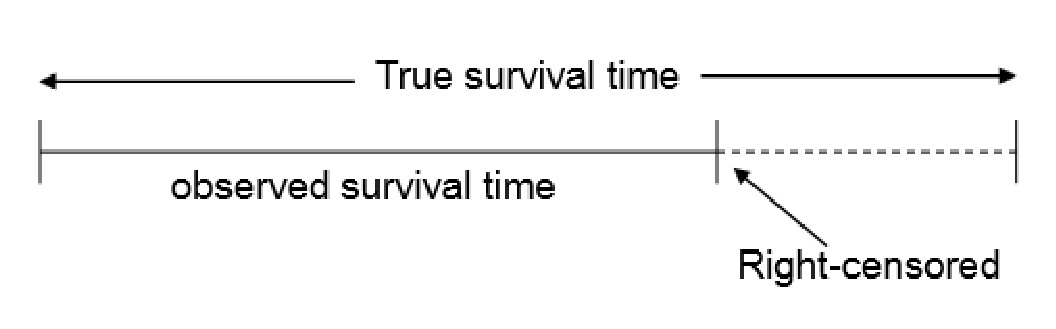
\includegraphics[height=2cm,
    angle=0]{./images/logrank_info.eps}}
  \caption{Log-rank test}
\label{fig:logrank_info}
\end{figure}

R code: \verb!survdiff! function
\begin{verbatim}
time <-c(6,6,6,7,10,13,16,22,23,6,9,10,11,17,19,20,25,32,32,34,35,1,1,2,2,3,4,4,5,5,8,8,8,8,11,11,
12,12,15,17,22,23)
status <-c(1,1,1,1,1,1,1,1,1,0,0,0,0,0,0,0,0,0,0,0,0,1,1,1,1,1,1,1,1,1,1,1,1,1,1,1,1,1,1,1,1,1)

treatment <-c(1,1,1,1,1,1,1,1,1,1,1,1,1,1,1,1,1,1,1,1,1,2,2,2,2,2,2,2,2,2,2,2,2,2,2,2,2,2,2,2,2,2)
fit <-survdiff(Surv(time, status) ~ treatment)
\end{verbatim}
The result
\begin{verbatim}
fit
Call: survdiff(formula = Surv(time, status) ~ treatment)
            N   Observed Expected (O-E)^2/E (O-E)^2/V
treatment=1 21  9        19.3     5.46      16.8
treatment=2 21  21       10.7     9.77      16.8

Chisq = 16.8 on 1 degrees of freedom, p = 4.17e-05
\end{verbatim}
In this example, the test is significant to reject H$_o$ (as the chance to
observe H$_o$ is too small).

Alternative methods (derived by applying different weights at the $j$-th
failure time, Fig.\ref{fig:logrank_weight}): Wilcoxen, Tarone-Ware, Peto,
Flemington-Harrington. So the question is \textcolor{red}{Which test to use?}: 
\begin{enumerate}
  \item The best choice is test with most power
  \item There may be a clinical reason to choose a particular weighting
  \item Choice of weight should be a priori (not fish for a desire p-value)
  \item Using different weights should usually give the same conclusion
\end{enumerate}

\begin{figure}[hbt]
  \centerline{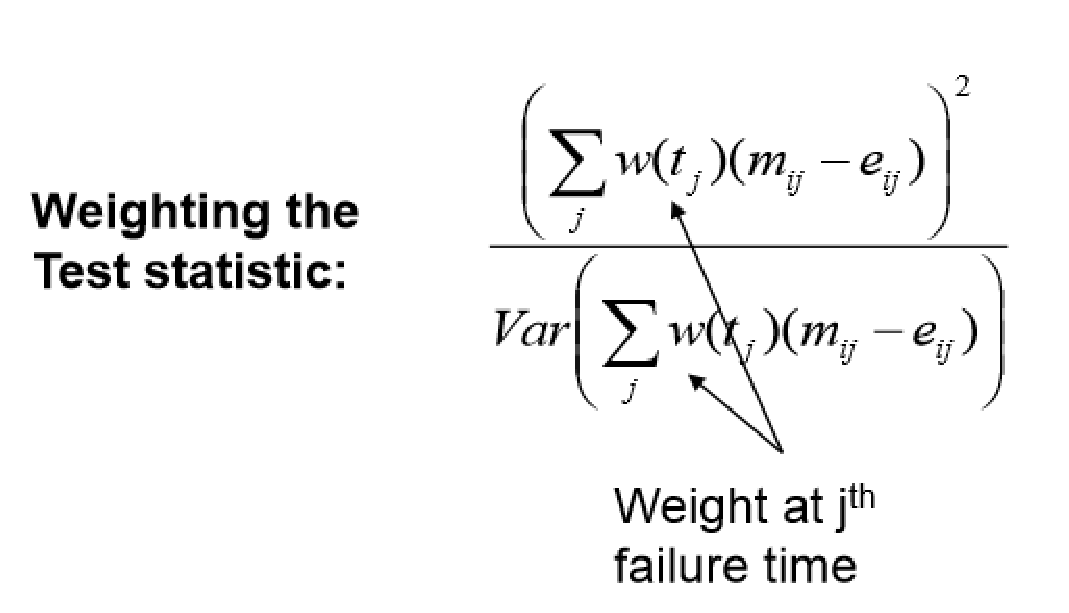
\includegraphics[height=3cm,
    angle=0]{./images/logrank_weight.eps}}
  \caption{Alternative to Log-rank test using weights}
\label{fig:logrank_weight}
\end{figure}

\url{http://stat.ethz.ch/education/semesters/ss2011/seminar/contents/presentation_2.pdf}

\subsection{Stratified logrank test}

When there is additional 'stratified' variable, data can be splitted based on
the value of stratified variable. In stratified logrank test, the data are
groupped into strata, Fig.\ref{fig:logrank_stratified}. So, $(O-E)$ are
calculated based on data within strata, and sum $(O-E)$ across strata. The
limitation is that sample size may be small with strata.


\begin{figure}[hbt]
  \centerline{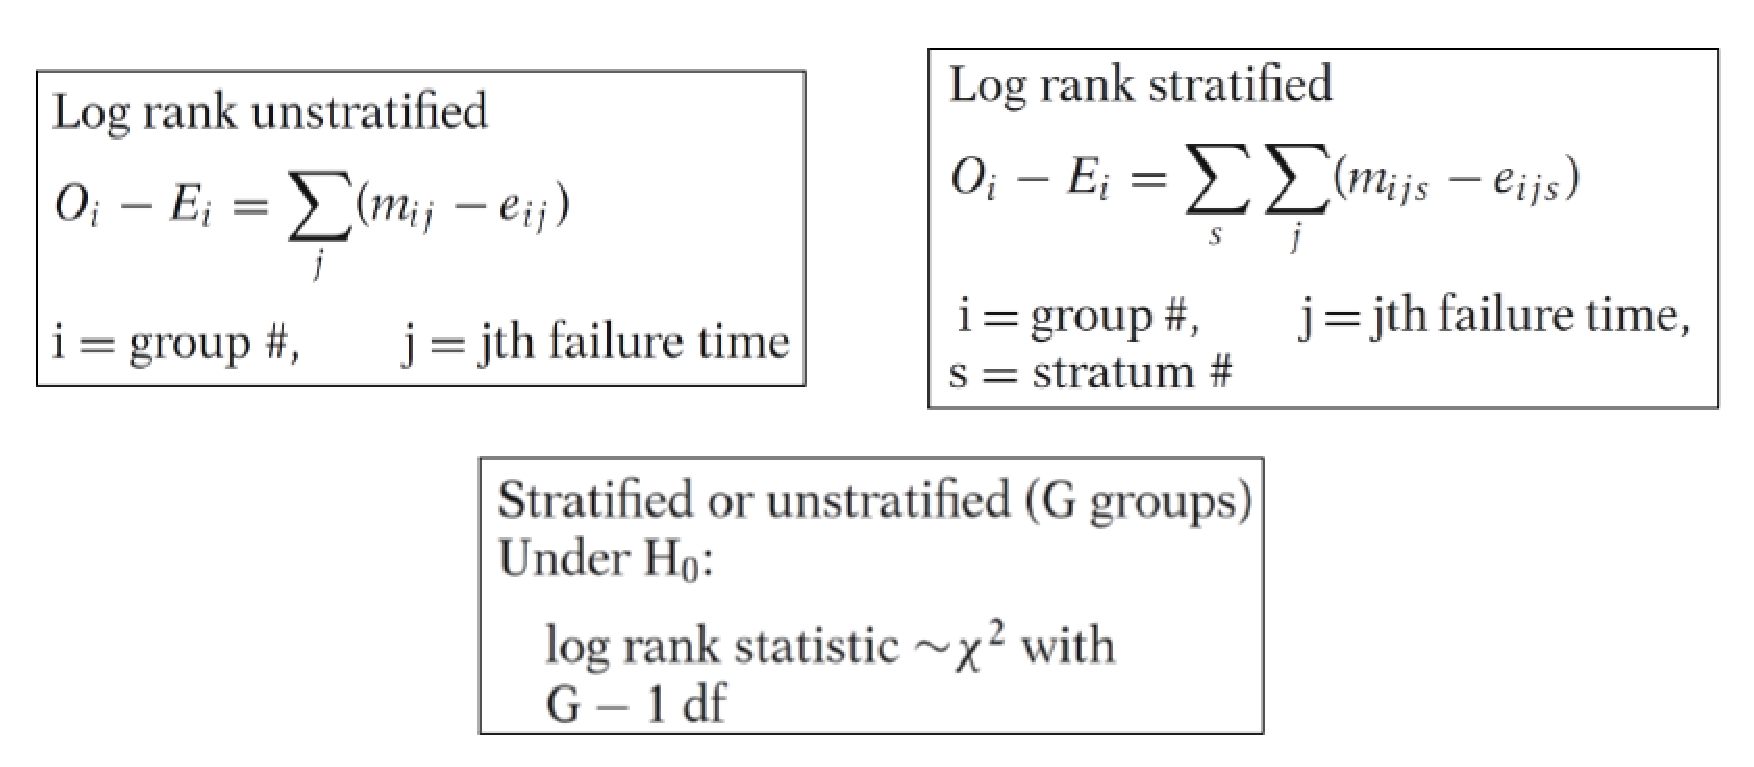
\includegraphics[height=3cm,
    angle=0]{./images/logrank_stratified.eps}}
  \caption{Comparison between stratified vs. unstratified logrank tests}
\label{fig:logrank_stratified}
\end{figure}


R code
\begin{verbatim}
data<-read.table("http://www.sph.emory.edu/~dkleinb/surv2datasets/anderson.dat")
lwbc3<-c(1,1,1,2,1,2,2,1,1,1,3,2,2,2,2,2,3,3,2,3,3,1,2,2,1,1,3,3,1,3,3,2,3,3,3,3,2,3,3,3,2,3)

fit <-survdiff(Surv(data$V1,data$V2)~data$V5+strata(lwbc3))
\end{verbatim}
The result is
\begin{verbatim}
fit 
Call: survdiff(formula = Surv(data$V1,data$V2)~ data$V5 + strata(lwbc3))

           N Observed Expected (O-E)^2/E (O-E)^2/V
data$V5=0 21 9        16.4      3.33      10.1
data$V5=1 21 21       13.6      4.00      10.1

Chisq =10.1 on 1 degrees of freedom,p =0.00145
\end{verbatim}

%%% Local Variables: 
%%% mode: latex
%%% TeX-master: "R_language"
%%% End: 

%%
%% ClassicGraphics.tex
%% Login : <hoang-trong@hoang-trong-laptop>
%% Started on  Sun Sep 20 18:55:26 2009 Hoang-Trong Minh Tuan
%% $Id$
%% 
%% Copyright (C) 2009 Hoang-Trong Minh Tuan
%%

\chapter{Classic Graphics}
\label{chap:classic-graphics}

Before starting with the gorgeous features of R language, we should
know how R graphic is organized. There are 4 different levels 
\begin{enumerate}
\item The highest level: graphical packages - (these are the packages
  whose functions we can call directly to plot graphs). Some of them
  are {\bf graphics}, {\bf maps}, {\bf lattice}, … in which the lattice package is
  very important and we will learn in the next chapter. In essence,
  all of the functions from these packages are built-upon the
  lower-level packages.

\item Next level: graphics systems - there are two subsystem
  (graphics, grid) from which we get the primitive functions for
  writing the user-end graphical functions. The grid graphic system is
  very important since the lattice package is written based on it. 

\item Next level: the graphic engine: {\bf grDevices}

\item The lowest level: Graphics Devices Packages (gtkDevice, …)

\end{enumerate}
Besides the traditional statistical plots ({\it scatterplots},
{\it boxplots}, {\it histograms}, {\it barblots}, {\it piecharts},
basic 3D plots), R provides an implementation of the
{\it Trellis plot}~\cite{becker1996vdc} via the packages lattice by
Deepayan Sarkar.

\section{Elementary graphic functions}
\label{sec:elem-graph-funct}

These special plots produce primitive graphics (lines, texts,
rectangles, and polygons). In essence, all complex graphics are
created from these primitive graphics. This makes it possible for
users to write their own functions.

One a graph is displayed; you can add several elements to it by using
these low-level functions.  

A new plot is created once you call a high-level plotting function or
{\bf frame()} command. 

\subsection{A straight line}
\label{sec:straight-line}

\begin{lstlisting}
abline(a = NULL, b = NULL, h = NULL, v = NULL, reg = NULL,
       coef = NULL, untf = FALSE, ...)
\end{lstlisting}

This can be used to draw horizontal or vertical line, with argument v
or h.

Example: Add one or more straight line through the current plot, e..g
the regression line {\bf lm()}


\subsection{Line segment}
\label{sec:line-segment}

\begin{lstlisting}
segments()
\end{lstlisting}

\subsection{Text}
\label{sec:text}

You can add text with the function {\bf text()} that takes at least 3
argument: (1) x-coordinate, (2) y-coordinate, (3) the text 
\begin{lstlisting}
text (x, y = NULL, labels = seq_along(x), adj = NULL,
     pos = NULL, offset = 0.5, vfont = NULL,
     cex = 1, col = NULL, font = NULL, ...)
\end{lstlisting}
If you don't know the location where to put the text, you can use the
{\bf locator()} function which will return the coordinates where you
click the mouse. And you just use the returned values to pass them as
the coordinates to the {\bf text()} function.


\subsection{Point}
\label{sec:point}

Add point or a marker to a specific coordinate

\begin{lstlisting}
points(x, y = NULL, type = "p", ...)
\end{lstlisting}

\subsection{An arrow}
\label{sec:an-arrow}

\begin{lstlisting}
arrows(x0, y0, x1, y1, length = 0.25, angle = 30, code = 2,
       col = par("fg"), lty = par("lty"), lwd = par("lwd"),
       ...)
\end{lstlisting}
Draw an arrow between a pair of points.

\subsection{Title to a plot}
\label{sec:title-plot}

Add a label (title) to a plot
\begin{lstlisting}
title(main = NULL, su	b = NULL, xlab = NULL, ylab = NULL,
      line = NA, outer = FALSE, ...)
\end{lstlisting}

A legend describes what each of the plotting symbol represents.
\footnote{\url{http://cspeech.ucd.ie/~fred/R/legend.html}}
\begin{lstlisting}
legend(x, y = NULL, legend, fill = NULL, col = "black", lty, lwd, pch,
       angle = NULL, density = NULL, bty = "o", bg = par("bg"),
       pt.bg = NA, cex = 1, xjust = 0, yjust = 1,
       x.intersp = 1, y.intersp = 1, adj = c(0, 0.5),
       text.width = NULL, merge = do.lines && has.pch, trace = FALSE,
       plot = TRUE, ncol = 1, horiz = FALSE)
\end{lstlisting}
\begin{verbatim}
     x, y: the coordinate of the upper left corner of the 
rectangle surrounding the legend
     legend = a vector of the text to be displayed for 
each curve on the plot
     col = a vector of color that representing the color
of each curve on the plot 
     text.col = color of the text on the legend
     lty = a vector of the line type of each curve 
(must be the same as the corresponding curve)
     pch = a vector of pch types that are used at each curve
     merge = TRUE then merge the points() and lines() 
if there are points() and lines () drawing for the curves on the plot
     bg = background color for the legend box
\end{verbatim}

{\bf Example}:
\begin{lstlisting}
plot(x, sin(x), type = "l", ylim = c(-1.2, 1.8), col = 3, lty = 2)
points(x, cos(x), pch = 3, col = 4)
lines(x, tan(x), type = "b", lty = 1, pch = 4, col = 6)

legend(-1, 1.9, legend = c("sin", "cos", "tan"), col = c(3,4,6),
       text.col = "green4", lty = c(2, -1, 1), pch = c(-1, 3, 4),
       merge = TRUE, bg = 'gray90')
\end{lstlisting}

\begin{figure}[hbt]
 \centerline{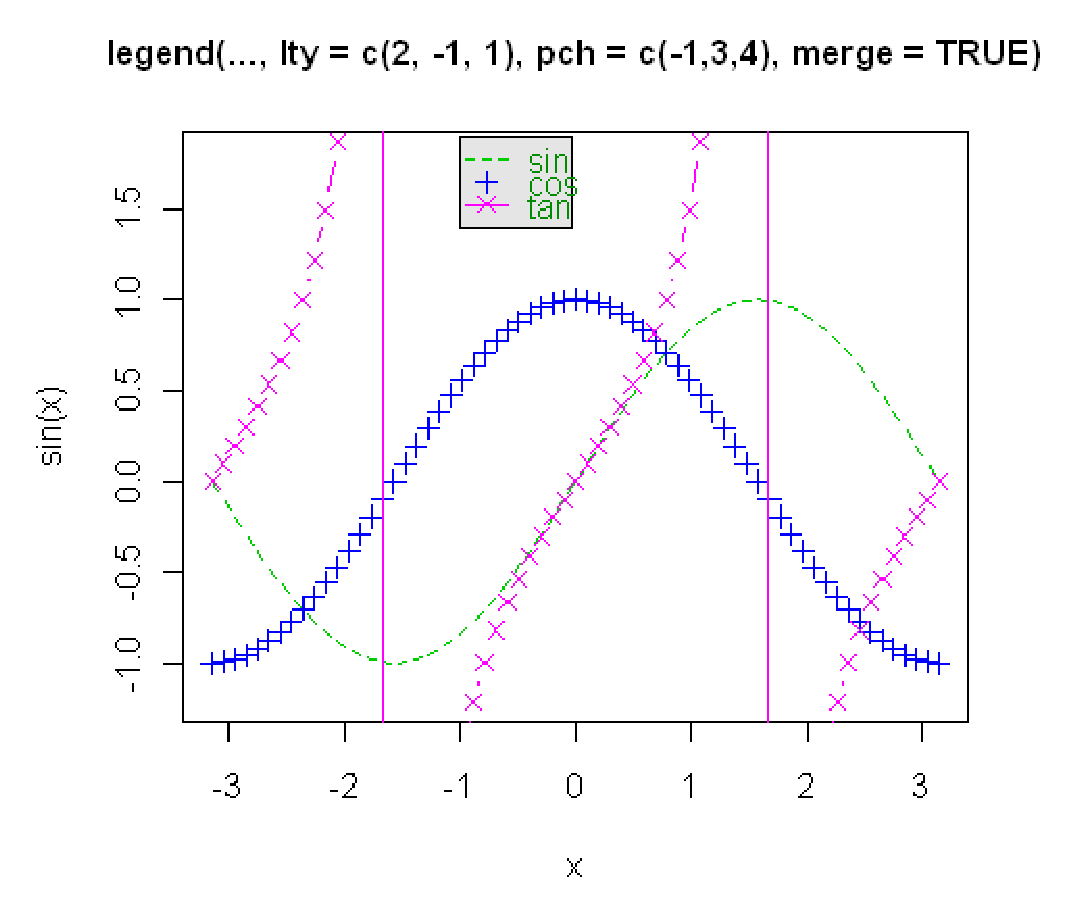
\includegraphics[height=5cm]{./images/legend.eps}}
\caption{Plot with a legend}
\label{fig:legend}
\end{figure}

If you don't know the location where to put the legend, you can use
the {\bf locator()} function which will return the coordinates where
you click the mouse. 

\subsection{Axis}
\label{sec:axis}

You can make any changes to axis (tick step, arrows, ...)
\begin{lstlisting}
axis(side, at = NULL, labels = TRUE, tick = TRUE, line = NA,
     pos = NA, outer = FALSE, font = NA, lty = "solid",
     lwd = 1, lwd.ticks = lwd, col = NULL, col.ticks = NULL,
     hadj = NA, padj = NA, ...)
\end{lstlisting}


\begin{itemize}
\item xpd=TRUE: normally, the tick at the far end are clipped at the plot region. So, if you want the tick at the far end to be drawn, enable this option
\end{itemize}

\subsection{A Box}
\label{sec:box}

You can add a box
\begin{lstlisting}
box()
\end{lstlisting}


\section{2D graphs}
\label{sec:2d-graphs}

\subsection{Boxplot}
\label{sec:boxplot}

There are two options: use the default function {\bf boxplot()} or the
function written in the {\it aplpack} package: {\bf boxplot2D()}

\begin{lstlisting}
boxplot(x, ..., range = 1.5, width = NULL, varwidth = FALSE,
        notch = FALSE, outline = TRUE, names, plot = TRUE,
        border = par("fg"), col = NULL, log = "",
        pars = list(boxwex = 0.8, staplewex = 0.5, outwex = 0.5),
        horizontal = FALSE, add = FALSE, at = NULL)
\end{lstlisting}
Visually display the summary of the distribution of the set of observations denoted by vector x.

Statistical issues:
\begin{itemize}
\item If we want to see how distribution of different variables in the
  same plot (e.g. there will be many box on the same plot), you need
  to group them with the function list() at the variable x 

\item range = this determines how far the plot whiskers extend out
  from the box (the values of zero causes the whisker extends to the
  data extremes \verb|->| there will be no outliers to be detected) 

\item plot = if FALSE, return the statistical summary of information
  from the plot, otherwise, return the plot 

\item notch = TRUE: draw the notch \verb|->| if the notches of two
  plots do not overlap this is 'strong evidence' that the two
  medians differ

\end{itemize}

Graphical issues:
\begin{itemize}
\item with = gives the relative width of the boxes making up the plot
varwidth is TRUE, the boxes are drawn with widths proportional to the
square-roots of the number of observations in the groups 

\item outline = to draw outline or not 

\item Add name to the graphs: set the parameter names
boxwex = scale all box \verb|->| improve visual performance when there
are a few box in the plot 

\item col = 

\item add = TRUE: add the boxplot to the current plot

\end{itemize}

{\bf Example}: 
\begin{lstlisting}
> boxplot(list(men, female), names = c("male", "female"))
\end{lstlisting}

NOTE: In the graph, points that are 'very extreme' are plotted by
themselves (outliers). Other data are represented


\section{Combine plots}
\label{sec:combine-plots}

\url{http://www.statmethods.net/advgraphs/layout.html}

%%% Local Variables: 
%%% mode: latex
%%% TeX-master: "R_language"
%%% End: 

%%
%% Packages.tex
%% Login : <hoang-trong@hoang-trong-laptop>
%% Started on  Fri Jun 12 19:41:23 2009 Hoang-Trong Minh Tuan
%% $Id$
%% 
%% Copyright (C) 2009 Hoang-Trong Minh Tuan
%% This program is free software; you can redistribute it and/or modify
%% it under the terms of the GNU General Public License as published by
%% the Free Software Foundation; either version 2 of the License, or
%% (at your option) any later version.
%% 
%% This program is distributed in the hope that it will be useful,
%% but WITHOUT ANY WARRANTY; without even the implied warranty of
%% MERCHANTABILITY or FITNESS FOR A PARTICULAR PURPOSE.  See the
%% GNU General Public License for more details.
%% 
%% You should have received a copy of the GNU General Public License
%% along with this program; if not, write to the Free Software
%% Foundation, Inc., 59 Temple Place, Suite 330, Boston, MA 02111-1307 USA
%%

\chapter{Packages}
\label{chap:packages}


\section{Dealing with a package}
\label{sec:dealing-with-package}

\subsection{Install a package}
\label{sec:install-package-1}


To install a package\footnote{\url{http://support.stat.ucla.edu/view.php?supportid=30 
}}.

\begin{lstlisting}
> install.packages("package_name")
\end{lstlisting}

Example: the {\it aplpack} package 
\begin{lstlisting}
> install.packages("aplpack")
\end{lstlisting}

\subsection{Load/Unload an installed package}
\label{sec:load-an-inst}

In R, there are many user defined packages. The system has some
automatically loadded/attached packages: base, stats, datasets...
\begin{table}
\begin{center}
  \begin{tabular}{cl}
    graphics & all functions to produce graphics \\
    grDevices & all functions to handle different devices for graphics
    \\
    datasets & objects from different sample data sets \\
    utils  & all standard R utility functions \\
    stats & all standard R functions for statistical data analysis \\
  \end{tabular}
\end{center}
\caption{Standard packages}
\end{table}


\textbullet List all loaded packages with {\bf search()}
\begin{lstlisting}
>> search() 
[1] ".GlobalEnv"        "package:stats"     "package:graphics" 
[4] "package:grDevices" "package:utils"     "package:datasets" 
[7] "package:methods"   "Autoloads"         "package:base" 
\end{lstlisting}
The first location, the package with index = 1, is always.GlobalEnv.

\textbullet List all loaded packages with {\bf sessionInfo()}
\begin{lstlisting}
>> sessionInfo()
R version 2.7.1 (2008-06-23) 
i486-pc-linux-gnu 

locale:
LC_CTYPE=en_US.UTF-8;LC_NUMERIC=C;LC_TIME=en_US.UTF-8;
LC_COLLATE=en_US.UTF-8;LC_MONETARY=C;LC_MESSAGES=en_US.UTF-8;
LC_PAPER=en_US.UTF-8;LC_NAME=C;LC_ADDRESS=C;LC_TELEPHONE=C;
LC_MEASUREMENT=en_US.UTF-8;LC_IDENTIFICATION=C 

attached base packages:
[1] stats     graphics  grDevices utils     datasets  methods   base 
\end{lstlisting}

\textbullet List all installed package, use {\bf library()} function
\begin{lstlisting}
>> library()
Packages in library '/usr/lib/R/library':

base                    The R Base Package
boot                    Bootstrap R (S-Plus) Functions (Canty)
class                   Functions for Classification
cluster                 Cluster Analysis Extended Rousseeuw et al.
codetools               Code Analysis Tools for R
datasets                The R Datasets Package
......
\end{lstlisting}

A function in a package should be used explicitly with its package
name in front. This is similar to using the variable within an object
(e.g. the column names within a data.frame object).  However, you can
load the package so that calling to the function can be used without
the package name.


\textbullet To load a package, use {\bf attach(obj), attach(lib.name)}
or {\bf library(lib.name)} function.
\begin{lstlisting}
>> library(cluster)
\end{lstlisting}

\textbullet Each loaded package is associated with an index value
(found in the {\it search()} function), user can use this value to
list all functions in that package using {\bf ls(pos=index)} function.
\begin{lstlisting}
> ls(2) # 2 is stats
 [1] "agnes"                   "agriculture"            
 [3] "animals"                 "bannerplot"             
 [5] "chorSub"                 "clara"                  
 [7] "clusplot"                "coef.hclust"            
 [9] "daisy"                   "diana"                  
[11] "ellipsoidhull"           "ellipsoidPoints"        
[13] "fanny"                   "flower"                 
[15] "lower.to.upper.tri.inds" "meanabsdev"             
[17] "mona"                    "pam"                    
[19] "plantTraits"             "pltree"                 
[21] "pluton"                  "predict.ellipsoid"      
[23] "ruspini"                 "silhouette"             
[25] "sizeDiss"                "sortSilhouette"         
[27] "upper.to.lower.tri.inds" "volume"                 
[29] "votes.repub"             "xclara"    
\end{lstlisting}

  \textbullet If you want the packages to be automatically loaded
  every time, there are 2 ways 

  \begin{enumerate}
  \item Click Packages\textbackslash Load and choose the
  package to load 
  \item Put it in the .First() function. This requires you
  to know the package name, use this below function to list the names
  of packages.  
\begin{lstlisting}
>> select.list(sort(.packages(all.available=TRUE)))
\end{lstlisting}
  Then, in the .First() function, add this line: \lstinline!library(lib_name)!
  \end{enumerate}

\section{Building a package}
\label{sec:building-package}

\begin{verbatim}
http://tldp.org/HOWTO/Debian-Binary-Package-Building-HOWTO/x60.html 
http://faculty.chicagogsb.edu/peter.rossi/research/bayes%20book/bayesm/Making%20R%20Packages%20Under%20Windows.pdf 
\end{verbatim}

\section{Packages for graphics}
\label{sec:packages-graphics}

\subsection{aplpack}
\label{sec:aplpack}


The name stands for {\it Another PLoting PACKage}\footnote{\url{http://www.wiwi.uni-bielefeld.de/~wolf/software/aplpack/}}

\begin{table}
\begin{center}
  \begin{tabular}{cl}
    
    stem.leaf & plots stem and leaf displays  \\
    bagplot &  plots bagplots  \\
    boxplot2D &  plots boxplots into a scatterplot  \\
    faces  & plots chernoff faces  \\
    spin3R &  for inspection of a 3-dim point cloud \\
  \end{tabular}
\end{center}
\caption{Functions in aplpack package}
\label{tab:aplpack}
\end{table}

\subsection{analogue \& vegan}
\label{sec:analogue--vegan}

Ordination methods, diversity analysis and other functions for
community and {\it vegetation ecologists}\footnote{\url{
http://www.jstatsoft.org/v22/i02}, \url{
http://bm2.genes.nig.ac.jp/RGM2/pkg.php?p=analogue}, \url{
http://cran.r-project.org/web/packages/vegan/index.html}}
\begin{lstlisting}
>>> granulo(ade4)              Granulometric Curves
>>> plot.roc(analogue)         Plot ROC curves and associated
>>> diagnostics
>>> roc(analogue)              ROC curve analysis
>>> colAUC(caTools)            Column-wise Area Under ROC
>>> Curve (AUC)
>>> DProc(DPpackage)           Semiparametric Bayesian ROC
                          curve analysis
>>> cv.enet(elasticnet)        Computes K-fold cross-validated
                          error curve for elastic net
>>> ROC(Epi)                   Function to compute and draw
                          ROC-curves.
>>> lroc(epicalc)              ROC curve
>>> cv.lars(lars)              Computes K-fold cross-validated
                          error curve for lars
>>> roc.demo(TeachingDemos)    Demonstrate ROC curves by
                          interactively building 
\end{lstlisting}
  
\subsection{MASS}
\label{sec:mass}

Authors: Venables and Ripley, 2002

The contour() and the persp() functions create contour plots, and three dimensional sur-
faces. Here, these functions are used to plot contours and 3-D graph of a surface fitted to a
set of topological measurements in topo (from the MASS package). First, a surface is fitted
to the data using the loess() function in R. The fitted surface is used to obtain predicted
values z over a 2-dimensional grid (named as topo.grid below). The R generic function
predict() is useful for this purpose. The function expand.grid() used below, creates a
data frame from all combinations of the two vectors x and y.
\begin{lstlisting}
> data(topo)
> topo
> topo.surf=loess(zx*y,topo,span=0.25)
> topo.surf
> topo.grid=list(x=seq(0,6.5,0.2),y=seq(0,6.5,0.2))
> topo.z=predict(topo.surf, expand.grid(topo.grid))
> contour(topo.grid$x,topo.grid$y,topo.z)
> points(topo)
> persp(topo.grid$x,topo.grid$y,topo.z)
> persp(topo.grid$x,topo.grid$y,topo.z,theta=40,phi=40)
\end{lstlisting}

\subsection{ROCR}
\label{sec:rocr}


28 performance measures are implemented, which can be freely combined
to form parametric curves such as {\it ROC curves},
{\it precision/recall curves}, or {\it lift curves}. Many options such
as curve averaging (for cross-validation or bootstrap), augmenting the
averaged curves by standard error bar or boxplots, labeling cutoffs to
the curve, or coloring curves according to cutoff \footnote{\url{http://rocr.bioinf.mpi-sb.mpg.de/}}.

\begin{figure}[htb]
  \centerline{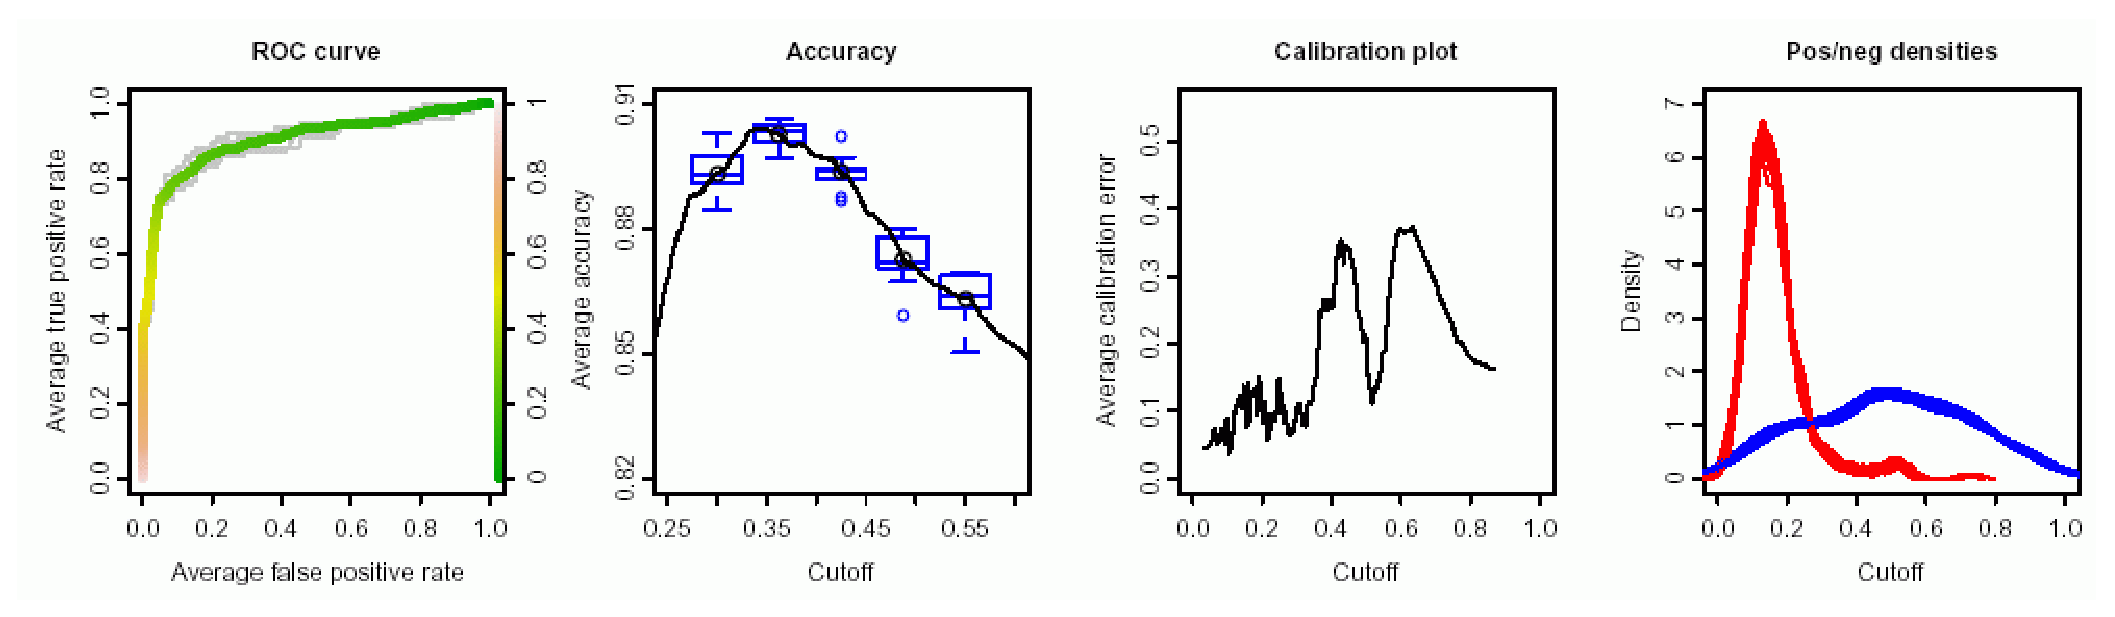
\includegraphics[height=5cm]{./images/ROCR_samples.eps}}
  \caption{Samples of ROC curves}\label{fig:ROCR_1}
\end{figure}

\section{Packages for data analysis}
\label{sec:pack-data-analys}

\subsection{BSDA}
\label{sec:bsda}
Basic Statistic and Data Analysis\footnote{\url{
http://cran.r-project.org/web/packages/BSDA/index.html}}
This contains the data and some statistic functions from the book 'Basic
statistics and data analysis', Kitchens, L. J. (2003) , Duxbury.

\subsection{coin}
\label{sec:coin}

coin stands for COnditional INference procedures in a permutation test
framework\footnote{\url{http://cran.r-project.org/web/packages/coin/index.html}}.
This package contains Conditional Inference Procedures for the general
independence problem including two-samples, K-sample (non-parametric
ANOVA), correlation, censored, ordered, and multivariate problems


\subsection{DAAG}
\label{sec:daag}

DAAG stands for Data Analysis And Graphics data and functions which
includes all functions described in the book Maindonald, J.H. and
Braun, W.J. (2003, 2007) "Data Analysis and Graphics Using R".

\subsection{nortest}
\label{sec:nortest}

nortest is being used to test for
normality\footnote{\url{http://cran.r-project.org/web/packages/nortest/index.html}}

\begin{lstlisting}
pearson.test(x, n.classes = ceiling(2 * (n^(2/5))), adjust = TRUE)
\end{lstlisting}

\subsection{sciplot}
\label{sec:sciplot}

The package "sciplot" is now available for download from CRAN. This
package includes a collection of functions that create graphs with
error bars for data collected from one-way or higher factorial
designs, as well as a function to plot bifurcation diagrams resulting
from analysis with XPPAUTO. The functions in this package replicate
some of the functionality of {\bf plotmeans()} from the package {\it gplots}, with
differences in the treatment of two-way and higher designs. Example
graphs can be seen at: \url{http://mutualism.williams.edu/sciplot}

\begin{figure}[htb]
    \centerline{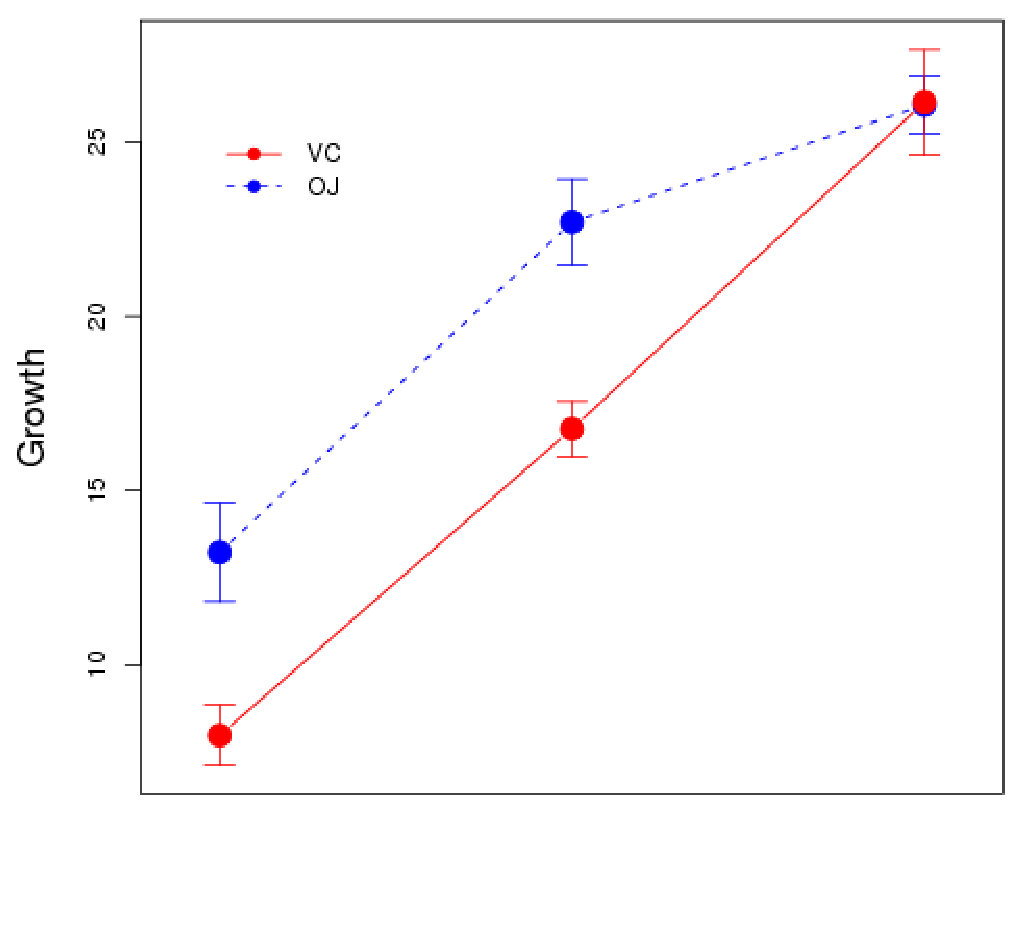
\includegraphics[height=5cm]{./images/sciplot_samples.eps}}
    \caption{Samples from sciplot}\label{fig:sciplot_1}
  \end{figure}

\section{Packages with problem solving}
\label{sec:pack-with-probl}

\subsection{plyr}
\label{sec:plyr}

{\bf plyr} is a set of tools that solves a common set of problems: you
need to break a big problem down into manageable pieces, operate on
each pieces and then put all the pieces back together.  It's already
possible to do this with {\bf split()} and the {\bf apply()}
functions, but plyr just makes it all a bit easier with:

\begin{itemize}
\item consistent names, arguments and outputs

\item input from and output to data.frames, matrices and lists

\item progress bars to keep track of long running operations

\item built-in error recovery

\item the choice of passing chunks as rows or as variables
\end{itemize}

plyr functions are named according to the type of object they input
(first letter) and output (second letter):

\begin{itemize}
\item   llply = from a list to a list
\item  alply = from an array (or vector, or matrix) to a list
\item  ldply = from a list to a data.frame
\item   \verb!d_ply! = from a data.frame, ignore output
\item and so on for llply, laply, ldply, \verb!l_ply!, alply, aaply,
  adply, \verb!a_ply!, dlply, daply, dply, \verb!d_ply!
\end{itemize}

plyr also provides:

\begin{itemize}
\item    m*ply which works in a similar way to mapply
\item   r*ply which works in a similar way to replicate
\end{itemize}

You can find out more at \url{http://had.co.nz/plyr/}, including a 20
page introductory guide\footnote{\url{http://had.co.nz/plyr/plyr-intro.pdf}}.


\section{Packages for model analysis}
\label{sec:pack-model-analys}

\subsection{Caret}
\label{sec:caret}

caret is a package for {\it building} and {\it evaluating} a wide
variety of predictive models. There are functions for pre-processing,
tuning models using resampling, visualizing the results, calculating
performance and estimating variable importance. 

{\bf caretNWS} and {\bf caretLSF} are two parallel processing versions
that can reduce the training time when multiple compute nodes are
available.

The project is now hosted on
\href{http://caret.r-forge.r-project.org/}{R-Forge}.  The package
currently includes {\bf model tuning/resampling} for the following
models: lm, single trees (C4.5, rpart, ctree, logistic model trees),
mars (via earth), boosted models (ada, gbm, blackboost, glmboost,
gamboost, logitboost), bagged models (trees, earth, fda),
randomforests (randomforest and cforest), rule-based models (Ripper
and M5 prime), discriminant models (lda, fda, rda, ssda, slda), kernel
methods (lssvm, ksvm, rvm, gausspr), nnet, nnet with initial pca step,
multinom, pls, plsda, gpls, nearest shrunken centroids, the lasso, the
elastic net, supervised pca, knn, lvq and NaiveBayes.

Recent changes include:
\begin{enumerate}
\item Estimation of class probabilities from PLS discriminant analysis
  using Bayes rule (in addition to softmax)
\item Added predict.train and predit.list

\item More lattice plots to visualize resampling results (xyplot,
  stripplot, densitplot, histogram) 

\item User-specified performance metrics for resampling

\item User-specified algorithms for determining the optimal tuning
  parameters (instead of highest/lowest)

\item A CHANGES files now exists to track the specifics of the version
  changes 
\end{enumerate}

\section{Packages for machine learning}
\label{sec:pack-mach-learn}

\subsection{e1071}
\label{sec:e1071}

Functions for latent class analysis, short time Fourier transform,
fuzzy clustering, support vector machines, shortest path computation,
bagged clustering, naive Bayes classifier, ...  
 
\subsection{GALGO}
\label{sec:galgo}

A package for multivariate variable selection using Genetic Algorithm
\url{http://www.bip.bham.ac.uk/bioinf/galgo.html }

\subsection{LearnBayes}
\label{sec:learnbayes}

\url{http://bm2.genes.nig.ac.jp/RGM2/pkg.php?p=LearnBayes}

\section{Packages in epidemiology}
\label{sec:pack-epid}

\subsection{epitools}
\label{sec:epitools}

\url{http://cran.r-project.org/web/packages/epitools/index.html}

\section{Packages in psychology}
\label{sec:packages-psychology}

\subsection{psych}
\label{sec:psych}


A number of routines for personality, psychometrics and experimental
psychology
research\footnote{\url{http://cran.r-project.org/web/packages/psych/index.html }}.
Functions are primarily for scale construction using factor analysis,
cluster analysis and reliability analysis, although others provide
basic descriptive statistics

\begin{lstlisting}
> install.packages("psych")
> library(psych)
\end{lstlisting}

Some useful functions:
\begin{lstlisting}
geometric.mean()
harmonic.mean()
\end{lstlisting}



%%% Local Variables: 
%%% mode: latex
%%% TeX-master: "R_language"
%%% End: 

\section{Miscellaneous}
\label{sec:miscellaneous}

\subsection{survey}
\label{sec:survey}

\url{http://faculty.washington.edu/tlumley/survey/}

\subsection{a}


\url{http://www.braju.com/R/}

\subsection{gplots}
\label{sec:gplots}


\section{Packages for bioinformatics}
\label{sec:pack-bioinf}

\subsection{Bioconductor}
\label{sec:bioconductor}

Bioconductor project (www.bioconductor.org)

%%
%% ValidateData.tex
%% Login : <hoang-trong@hoang-trong-laptop>
%% Started on  Sun Jun 14 16:39:43 2009 Hoang-Trong Minh Tuan
%% $Id$
%% 
%% Copyright (C) 2009 Hoang-Trong Minh Tuan
%% This program is free software; you can redistribute it and/or modify
%% it under the terms of the GNU General Public License as published by
%% the Free Software Foundation; either version 2 of the License, or
%% (at your option) any later version.
%% 
%% This program is distributed in the hope that it will be useful,
%% but WITHOUT ANY WARRANTY; without even the implied warranty of
%% MERCHANTABILITY or FITNESS FOR A PARTICULAR PURPOSE.  See the
%% GNU General Public License for more details.
%% 
%% You should have received a copy of the GNU General Public License
%% along with this program; if not, write to the Free Software
%% Foundation, Inc., 59 Temple Place, Suite 330, Boston, MA 02111-1307 USA
%%


\chapter{Validate Data}
\label{chap:validate-data}

\section{NaN, NA}
\label{sec:nan-na}

\subsection{NA}
\label{sec:na}


Missing values in the statistical sense are values that not known, NA.
The default type of NA is {\it logical}. So, the occurrence of NA may
trigger a logical rather than a numerical indexing. However, it may get coerced
to another type.

\begin{lstlisting}
if (na.rm)

        x <- x[!is.na(x)]

    else if (any(is.na(x)))
        stop("Missing values and NaN's not allowed if `na.rm' is FALSE")
    if (any((p.ok <- !is.na(probs)) & (probs < 0 | probs > 1))) 
        stop("probs outside [0,1]")
    if (na.p <- any(!p.ok)) {
        o.pr <- probs
        probs <- probs[p.ok]
\end{lstlisting}

Any numerical or logical calculation with NA generally return NA.

NA is not comparable to any values, including itself. So, to test for
the missing value of an object or entry, {\bf is.na()} function is
used. However, in matching, a NA value will match a NA value.

(since R 1.5.0) A string `NA' is different from a NA character
type. So, to specify a NA character type, use
\begin{lstlisting}
as.character(NA)
\end{lstlisting}

(since R 2.5.0) To use a NA value of appropriate type, there are some
new constants: \lstinline!NA_integer_, NA_real_, NA_complex_,!
\lstinline!NA_character_!.


\subsection{NaN}
\label{sec:nan}

Numerical calculation whose result is undefined, e.g. $0/0$, produce
the value NaN. To check for an object/expression is NaN, {\bf
  is.nan(object)} is used, {\bf is.na(NaN)} return TRUE. 

Coercing NaN to integer or logical type result in a NA value. However
coercing it to a character type result in a `NaN` string. 

Any comparison with NaN value result in a NA value (logical). 

A NaN value only match to another NaN value, not NA.



%%% Local Variables: 
%%% mode: latex
%%% TeX-master: "R_language"
%%% End: 


\part{R for numerical computing}
%%
%% NumericalRecipe.tex
%% Login : <hoang-trong@hoang-trong-laptop>
%% Started on  Thu Jul 16 17:18:19 2009 Hoang-Trong Minh Tuan
%% $Id$
%% 
%% Copyright (C) 2009 Hoang-Trong Minh Tuan
%%

\chapter{Numerical recipes in R}
\label{chap:numerical-recipes-r}

\section{Solving system of ODE}
\label{sec:solving-system-ode}

You can use {\bf lsoda()}
function\footnote{\url{http://hosho.ees.hokudai.ac.jp/~kubo/Rdoc/library/odesolve/html/lsoda.html}}.
\begin{lstlisting}
lsoda(y, times, func, parms, rtol, atol, tcrit=NULL, 
  jacfunc=NULL, verbose=FALSE, dllname=NULL, hmin=0, 
  hmax=Inf, ...)

\end{lstlisting}

This function, indeed, call the Fortran subroutine {\bf lsoda}, from Netlib.

%%% Local Variables: 
%%% mode: latex
%%% TeX-master: "R_language"
%%% End: 

%%
%% Parallel.tex
%% Login : <hoang-trong@hoang-trong-laptop>
%% Started on  Mon Jun 22 21:51:55 2009 Hoang-Trong Minh Tuan
%% $Id$
%% 
%% Copyright (C) 2009 Hoang-Trong Minh Tuan
%% This program is free software; you can redistribute it and/or modify
%% it under the terms of the GNU General Public License as published by
%% the Free Software Foundation; either version 2 of the License, or
%% (at your option) any later version.
%% 
%% This program is distributed in the hope that it will be useful,
%% but WITHOUT ANY WARRANTY; without even the implied warranty of
%% MERCHANTABILITY or FITNESS FOR A PARTICULAR PURPOSE.  See the
%% GNU General Public License for more details.
%% 
%% You should have received a copy of the GNU General Public License
%% along with this program; if not, write to the Free Software
%% Foundation, Inc., 59 Temple Place, Suite 330, Boston, MA 02111-1307 USA
%%

\chapter{Parallel R simulation}
\label{chap:parall-r-simul}


\url{https://csgillespie.github.io/efficientR/performance.html}

\begin{verbatim}
library("microbenchmark")
library("ggplot2movies")
library("profvis")
library("Rcpp")


library("profvis")
profvis({
  data(movies, package = "ggplot2movies") # Load data
  movies = movies[movies$Comedy == 1,]
  plot(movies$year, movies$rating)
  model = loess(rating ~ year, data = movies) # loess regression line
  j = order(movies$year)
  lines(movies$year[j], model$fitted[j]) # Add line to the plot
})
\end{verbatim}

\section{In Windows}
\label{sec:windows}

\begin{lstlisting}
cl <- makeCluster(2,type="SOCK")
\end{lstlisting}


\section{In Linux}
\label{sec:linux}

purpose-made packages for R : Snow, Rmpi, snowfall,...

\section{serial versions}


When you have a list of repetitive tasks, if each task is completely independent
of the others, then it is a prime candidate for executing those tasks in
parallel, each on its own core.

\url{https://nceas.github.io/oss-lessons/parallel-computing-in-r/parallel-computing-in-r.html}

Example: iris data with 5 columns
\begin{verbatim}
> iris
    Sepal.Length Sepal.Width Petal.Length Petal.Width    Species

1
2
.
.
.
150
\end{verbatim}

Example:
\begin{verbatim}
# return row indices in that the fifth-column
which(iris[,5] != "setosa")

# ... then extract 1st and 5th columns on those rows
x <- iris[which(iris[,5] != "setosa"), c(1,5)]

\end{verbatim}


Example: multiple tasks in serial
\begin{verbatim}

trials <- 10000

res <- data.frame()


system.time({
  trial <- 1
  while(trial <= trials) {
    ind <- sample(100, 100, replace=TRUE)
    result1 <- glm(x[ind,2]~x[ind,1], family=binomial(logit))
    r <- coefficients(result1)
    res <- rbind(res, r)
    trial <- trial + 1
  }
})
\end{verbatim}

\section{lapply() versions - faster than loop}

In R, using \verb!apply()! is often significantly faster than the equivalent
code in a loop. To do that, we need to convert our task to a function, and then
use the \verb!*apply()! family of R functions to apply that function to all of
the members of a set.
\begin{verbatim}

trials <- seq(1, 10000)  #MUST BE A SEQUENCE NOW

system.time({

  results <- lapply(trials, boot_fx)
})

\end{verbatim}

\section{mcapply() versions - faster than loop}

Use the multiple cores on a local computer through mclapply,
which is analogous to lapply, but distributes the tasks to multiple processors.


The parallel library can be used to send tasks (encoded as function calls) to
each of the processing cores on your machine in parallel.

mclapply gathers up the responses from each of these function calls, and returns
a list of responses that is the same length as the list or vector of input data
(one return per input item).



\section{makeCluster, clusterApply}

Use multiple processors on local (and remote) machines using makeCluster and clusterApply

\begin{verbatim}
In this approach, one has to manually copy data and code to each cluster member using clusterExport

This is extra work, but sometimes gaining access to a large cluster is worth it

\end{verbatim}



\section{foreach library}


\section{doParallel library}



%%% Local Variables: 
%%% mode: latex
%%% TeX-master: "R_language"
%%% End: 


\part{Interoperability}
%%
%% InterLanguageComm.tex
%% Login : <hoang-trong@hoang-trong-laptop>
%% Started on  Thu Jul 16 17:34:44 2009 Hoang-Trong Minh Tuan
%% $Id$
%% 
%% Copyright (C) 2009 Hoang-Trong Minh Tuan
%%

\chapter{Inter-Language Communication}
\label{chap:inter-lang-comm}


To make a call to compiled code that has been loaded to R, you can
use\footnote{\url{http://hosho.ees.hokudai.ac.jp/~kubo/Rdoc/library/base/html/Foreign.html}}.
\begin{lstlisting}
.C(name, ..., NAOK = FALSE, DUP = TRUE, PACKAGE, ENCODING)
.Fortran(name, ..., NAOK = FALSE, DUP = TRUE, PACKAGE, ENCODING)
.External(name, ..., PACKAGE)
    .Call(name, ..., PACKAGE)

.External.graphics(name, ..., PACKAGE)
    .Call.graphics(name, ..., PACKAGE)
\end{lstlisting}

\section{Load a library}
\label{sec:load-library}

Here, you will know how to load a DLL (shared library) written in
another language (C, Fortran) into R. You use {\bf dyn.load()}
function\footnote{\url{http://hosho.ees.hokudai.ac.jp/~kubo/Rdoc/library/base/html/dynload.html}}.
\begin{lstlisting}
dyn.load(x, local = TRUE, now = TRUE, ...)
dyn.unload(x)

is.loaded(symbol, PACKAGE = "", type = "")
\end{lstlisting}


%%% Local Variables: 
%%% mode: latex
%%% TeX-master: "R_language"
%%% End: 

%%
%% Documentation.tex
%% Login : <hoang-trong@hoang-trong-laptop>
%% Started on  Mon Jun 22 21:42:54 2009 Hoang-Trong Minh Tuan
%% $Id$
%% 
%% Copyright (C) 2009 Hoang-Trong Minh Tuan

\chapter{Document your code}
\label{chap:document-your-code-1}



This is a very important part if you want your code to be useful to
others or later use.  Suppose that you have written your own function
mypow
\begin{lstlisting}
  mypow <- function(x, power) x^power
\end{lstlisting}

Now, you can use the command {\bf prompt(func\_name)} to document your function

\begin{lstlisting}
> prompt (mypow)
\end{lstlisting}
You will see something like this\footnote{\url{http://www.hsph.harvard.edu/biostats/courses/individual/bio271/lectures/L6/L6.pdf}}.
\begin{verbatim}
created file named mypow.Rd in the current directory
  Edit the file and move it to the appropriate directory, 
possibly /usr4/biostatistics/src/R-1.4.1/src/library/<pkg>/man/
\end{verbatim}


%%% Local Variables: 
%%% mode: latex
%%% TeX-master: "R_language"
%%% End: 

%%
%% MissingFeature.tex
%% Login : <hoang-trong@hoang-trong-laptop>
%% Started on  Mon Jun 22 11:02:20 2009 Hoang-Trong Minh Tuan
%% $Id$
%% 
%% Copyright (C) 2009 Hoang-Trong Minh Tuan
%% This program is free software; you can redistribute it and/or modify
%% it under the terms of the GNU General Public License as published by
%% the Free Software Foundation; either version 2 of the License, or
%% (at your option) any later version.
%% 
%% This program is distributed in the hope that it will be useful,
%% but WITHOUT ANY WARRANTY; without even the implied warranty of
%% MERCHANTABILITY or FITNESS FOR A PARTICULAR PURPOSE.  See the
%% GNU General Public License for more details.
%% 
%% You should have received a copy of the GNU General Public License
%% along with this program; if not, write to the Free Software
%% Foundation, Inc., 59 Temple Place, Suite 330, Boston, MA 02111-1307 USA
%%

\chapter{Missing features}
\label{chap:missing-features}

\section{Function argument}
\label{sec:function-argument}


\subsection{Multivariate functions}
\label{sec:mult-funct}

Current
\begin{lstlisting}
f = function(v){ v[1]^2 + 2*v[1]*v[2] + sqrt(v[3])*v[1] }
\end{lstlisting}
Expected:
\begin{lstlisting}
f = function([x,y,z]){ x^2 + 2*x*y + sqrt(z)*x }
\end{lstlisting}

\section{Matrix}
\label{sec:matrix-1}

\subsection{Assembling matrices}
\label{sec:assembling-matrices}

Current
\begin{lstlisting}
> M = cbind( rbind(1,2,3), rbind(6,5,4) )
----------------
     [,1] [,2]
[1,]   1   6
[2,]   2   5
[3,]   3   4
\end{lstlisting}
Expected: a concise operator for assembling matrix

\subsection{MatLab-like consistency}
\label{sec:matl-like-cons}

Current
\begin{lstlisting}
> M[,1]
[1] 1 2 3
\end{lstlisting}
Expected: if you extract a column, it should return a column (not a row)



%%% Local Variables: 
%%% mode: latex
%%% TeX-master: "R_language"
%%% End: 


\part{Machine Learning}
\import*{../Big_Data/}{DeepLearning.tex}
\import*{../Big_Data/}{MachineLearning.tex}


% \include{Data-types}

% \include{ProgramConstruct}

% \include{Subprograms}
% %%
%% Files.tex
%% Login : <hoang-trong@hoang-trong-laptop>
%% Started on  Fri Jun 12 19:40:46 2009 Hoang-Trong Minh Tuan
%% $Id$
%% 
%% Copyright (C) 2009 Hoang-Trong Minh Tuan
%% This program is free software; you can redistribute it and/or modify
%% it under the terms of the GNU General Public License as published by
%% the Free Software Foundation; either version 2 of the License, or
%% (at your option) any later version.
%% 
%% This program is distributed in the hope that it will be useful,
%% but WITHOUT ANY WARRANTY; without even the implied warranty of
%% MERCHANTABILITY or FITNESS FOR A PARTICULAR PURPOSE.  See the
%% GNU General Public License for more details.
%% 
%% You should have received a copy of the GNU General Public License
%% along with this program; if not, write to the Free Software
%% Foundation, Inc., 59 Temple Place, Suite 330, Boston, MA 02111-1307 USA
%%

\chapter{Files}
\label{chap:files}

Reading data into a statistical analysis system and export the result
to some other system are essential tasks.  In general, a data set is
organized in column-wise. As a matter of fact, data file should also
be organized in a format such that elements can be detected easily and
organized into columns.

If the file is a text file, each row is a record. In a single line,
there is a delimiter (tab, whitespace...)  to separate elements in a
row. Tab-separated and whitespace-separated text file is an important
part of working with R. To read/write to these text files, R provides
2 functions: {\bf read.table()} and {\bf write.table()}.

R is not really good in manipulating large-scale data. Thus, it is
recommended to use the facilities provided by other languages,
e.g. Java, Perl or Python, and then make use of the packages written
in these languages from R. Some of them includes: SJava, RSPerl,
RSPython packages from \href{http://www.omegahat.org}{OmegaHat}
project; and rJava from CRAN.

% R is not well suit for large-scale data. Thus, there are several
% packages (SJava, RSPerl, RSPython - from Omegahat project, and rJava -
% from CRAN) that allows user to integrate Python, Perl, Java... codes
% into R.

Normally, the files are {\it tab-separated} or {\it
  whitespace-separated} text files.  

\section{Excel file}

For writing to Excel file, it's best to use \verb!openxlsx! as it is not Java-depdendent.

For reading Excel file, it is best to use  \verb!readxl! package

\subsection{openxlsx}

 Through the use of 'Rcpp', read/write times are comparable to the 'xlsx' and
 'XLConnect' packages with the added benefit of removing the dependency on Java.
 
\url{https://cran.r-project.org/web/packages/openxlsx/}


\subsection{readxl package}
\label{sec:readxl-package}

Readxl and Rcpp are needed to load an .xls or .xlxs file.

\begin{verbatim}
> install.package(readxl)
# or
install.packages("tidyverse")

> library(readxl)
> readxl_example()
 [1] "clippy.xls"    "clippy.xlsx"   "datasets.xls"  "datasets.xlsx"
 [5] "deaths.xls"    "deaths.xlsx"   "geometry.xls"  "geometry.xlsx"
 [9] "type-me.xls"   "type-me.xlsx" 
\end{verbatim}


\section{Import}
\label{sec:import}

\subsection{into a vector or list}
\label{sec:into-vector-or}

You can read data from a file into a vector or a list using
{\bf scan()} command. The default is {\it whitespace-separated}
file. You can tell a different delimiter using {\it sep}
parameter. You can also skip a number of lines before starting to read
data by using {\it skip} parameter. You can also tell the maximum
number of lines of data to be read using {\it nlines} parameter.

\begin{lstlisting}
 scan(file = "", what = double(0), nmax = -1, n = -1, sep = "",
          quote = if(identical(sep, "\n")) "" else "'\"", dec = ".",
          skip = 0, nlines = 0, na.strings = "NA",
          flush = FALSE, fill = FALSE, strip.white = FALSE,
          quiet = FALSE, blank.lines.skip = TRUE, multi.line = TRUE,
          comment.char = "", allowEscapes = FALSE,
          encoding = "unknown")
\end{lstlisting}
{\it what} tells the type of data to be read (which can be either
'logical', 'integer', 'numeric', 'complex', 'character', 'raw' and
'list').

{\bf IMPORTANT}: If {\it what} is a 'list', then each line is a record
which contains length, fields and the list components which must be of
either 6 types listed.

{\it nmax} is the maximum number of values to read. By default, it
reads all. 

{\bf IMPORTANT}: If {\it what} is a 'list', then {\it nmax} tells the
number of lines (records) to read. 

\subsection{into a data.frame}
\label{sec:into-data.frame}

The data from the file is organized in table format, i.e. it can have
a header row, and row names. Thus, we have to use {\bf read.table()}
command. 

\begin{lstlisting}
read.table(file, header = FALSE, sep = "", 
           quote = "\"'", dec = ".", 
           row.names, col.names,
           as.is = !stringsAsFactors,
           na.strings = "NA", colClasses = NA, 
           nrows = -1, skip = 0, check.names = TRUE, 
           fill = !blank.lines.skip,
           strip.white = FALSE, 
           blank.lines.skip = TRUE,
           comment.char = "#",
           allowEscapes = FALSE, flush = FALSE,
           stringsAsFactors = default.stringsAsFactors(),
           encoding = "unknown")
\end{lstlisting}
By default: there is no header row (header=FALSE), the file is {\it
  whitespace-separated}. If there is a column read as character
string, we need to specify the quoting character using {\it quote}
parameter. 

As the data is in table format, it can have row names which can be
specified through a vector (using {\it row.names} assigned to a
vector), a number which tells the columns in the file that contains
row names (using {\it row.names} assigned to a column number), a
character string which is the name of a table column whose elements
are row names (using {\it row.names} assigned to a character string,
and {\it header}=TRUE). If {\it header}=TRUE, and the number of fields
in the first row is less than the number of columns in the data, then
the first column in the data is designated for row names. Otherwise,
row names are automatically numbered with 1, 2, 3.... 


\section{Export to a text file}
\label{sec:export-text-file}

The primary function is {\bf cat()}. 


\section{Export to a binary file}
\label{sec:export-binary-file}


\url{http://cran.r-project.org/doc/manuals/R-data.html}

%%% Local Variables: 
%%% mode: latex
%%% TeX-master: "R_language"
%%% End: 

% \include{Compile}

% \include{Debug}

%\part{Appendix}
%\include{Appendix}

% Convention:

% \begin{itemize}
% \item Text with \textcolor{red}{red color}: obsolete feature,
%   statement...
% \item Text with \textcolor{green}{yellow color}: not available in this version
% \end{itemize}
\backmatter 
%\include{glossary}
%\include{notat}
\bibliographystyle{amsalpha} %The style you want to use for references.
\bibliography{ref_statistic} %The files containing all
                                %the articles and books you ever
                                %referenced. 
\printindex %Make an index AUTOMATICALLY

\end{document} 


%%% Local Variables: 
%%% mode: latex
%%% TeX-master: t
%%% End: 
